\documentclass[master,openright,oneside,color]{buaathesis}
\usepackage{booktabs}
\usepackage{graphicx}
\usepackage[ruled]{algorithm2e} % For algorithms
\usepackage{epstopdf}


\renewcommand{\algorithmcfname}{算法}
\makeatletter
\renewcommand{\@algocf@capt@plain}{above}% formerly {bottom}
\makeatother
\SetKwInput{KwData}{输入}
\SetKwInput{KwResult}{输出}
\setmainfont{Times New Roman}


\begin{document}

% 用户信息
% !Mode:: "TeX:UTF-8"

% 学院中英文名,中文不需要“学院”二字
% 院系英文名可从以下导航页面进入各个学院的主页查看
% http://www.buaa.edu.cn/xyykc/index.htm
\school
{计算机}{School of Computer Science \& Engineering}

% 专业中英文名
\major
{计算机应用技术}{Computer Science and Technology}

% 论文中英文标题
\thesistitle
{基于知识库和强化学习的代表性话题抽取研究}
{}
{Representative Topics Extraction Based on Knowledge Base and Reinforcement Learning}
{}

% 作者中英文名
\thesisauthor
{韩京飞}{Jingfei Han}

% 导师中英文名
\teacher
{荣文戈}{Rong Wenge}
% 副导师中英文名
% 注:慎用‘副导师’,见北航研究生毕业论文规范
%\subteacher{副导师}{subteacher}

% 中图分类号,可在 http://www.ztflh.com/ 查询
\category{TP391}

% 本科生为毕设开始时间;研究生为学习开始时间
\thesisbegin{2016}{09}{01}

% 本科生为毕设结束时间;研究生为学习结束时间
\thesisend{2019}{}{}

% 毕设答辩时间
\defense{2019}{}{}

% 中文摘要关键字
\ckeyword{层次概率,神经语言模型,递归神经网络,自然语言处理}

% 英文摘要关键字
\ekeyword{Hierarchical Softmax, Neural Language Model, Recurrent Neural Network, Natural Language Processing.}
% !Mode:: "TeX:UTF-8"

% 研究方向
\direction{自然语言处理}

% 导师职称中英文
\teacherdegree{副教授}{Associate Prof.}
% 副导师职称中英文
% 注:慎用‘副导师’,见北航研究生毕业论文规范
%\subteacherdegree{讲师}{Teacher}

% 保密等级,注:非保密论文时不需要此项
%保密论文请更改‘buaathesis.cls’里相应代码
%\mibao{机密}

%申请学位级别
\applydegree{工学硕士}

% 论文编号,由10006+学号组成
\thesisID{10006SY1606405}

% 论文提交时间
\commit{2019}{}

% 学位授予日期
\award{2019}{}{}


% 中英封面、提名页、授权书
\maketitle
% 前言页眉页脚样式
\pagestyle{frontmatter}
% 摘要
%\begin{cabstract}
%~\
%
%随着深度学习技术的发展,出现了丰富多样的基于神经网络的自然语言模型,这些神经网络模型一般都是通过学习大规模语料库来调整自身的参数分布,以提高模型在相关任务上的性能和精度。然而,对于目前的一些较大规模应用而言,语言模型的训练过程还显得较为缓慢,效率需要进一步提高。导致计算缓慢的原因是这些模型在训练和测试的时候,通常需要预测整个词表的单词从而选择出最佳的候选单词,该步骤占用了绝大部分计算资源和时间,一般称为大词表问题。为了应对这个挑战,研究人员提出了各种不同类型的方案,如:单词拆分算法、基于抽样的近似算法和层次概率模型等,其中层次概率模型只关注局部概率,可以很大程度降低训练和测试过程中所占用的计算资源,因此获得了广泛的关注。
%
%针对大词表问题,为了减少模型的计算时间并提高模型效率,本论文探讨了基于二叉树和基于类别的两种层次概率模型,并设计了相应的改进策略,其主要改进要点包括:1)提出了一种改进的层次模型的编码策略,引入基于树和基于类的并行度更高的损失函数;2)针对层次化模型对于聚类算法的敏感性问题,对基于N-gram、句法信息和语义信息的不同聚类算法对各种层次概率模型产生的影响进行了分析;3)对多种不同的结构化预测算法进行了分析,同时分析了语言模型在排序和打分两个任务中的选择策略。
%
%在实验验证环节,本文在语言建模任务上进行了评测,采用~WikiText-2, WikiText-103~和~One Billion Words~数据集作为实验的基准数据。在模型的评价指标方面,本文不仅考虑了传统的困惑度误差,还将文本比较中经常用到的编辑距离(单词错误率)作为一个重要的比较指标。除此之外,还比较了不同模型之间的训练和测试阶段内存占用量,以及相同数据量情况下模型的计算速度和模型的收敛速度等衡量指标。结果表明,与其他概率归一化方法相比,本文提出的层次概率算法具有很好的计算速度提升效果。同时还讨论了两种层次概率模型的适用范围和两者的优缺点。
%\end{cabstract}
%
%\begin{eabstract}
%~\
%
%Recent decades has witnessed great progress and achievements, in the field of natural language processing. Variants of neural networks based architecture have been proposed and successfully applied to the neural language models, neural acoustic models, neural translation model and etc. These neural models can leverage knowledge in texts by learning parameters from massive corpora, and abundant cases are presented over various text tasks, like sentence classification and word vector learning. While they are extremely slow for the real-world challenge, as they try to predict candidates from a large vocabulary, in the process of training and inference. As an alternative to vocabulary truncation and sampling-based approximation methods, we explore historical proposed tree-based and class-based hierarchical softmax methods.
%
%In this research, aiming at reducing neural model's computational time as well as making them compatible with modern devices, we introduce a series of efficient approaches and categorise our contributions as: a) Firstly, we reform their structural composition and introduce a compact tree-based loss function for the tree-based hierarchical softmax methods and class-based loss function for the corresponding class-based hierarchical softmax; b) Then, we discuss the impact of several ngram-based, syntactic and semantic clustering algorithms for the vanilla hierarchical softmax as these structural models are sensitive to the hierarchical clustering methods; c) Thirdly, we discuss possible inference algorithms for the hierarchical softmax variants, assuring the model can fetch presumable predictions under different circumstances.
%
%Finally, Our experiments were carried out on language modelling tasks with standard benchmarks datasets, i.e., WikiText-2, WikiText-103 and One Billion Words datasets. Except for the traditional perplexity metric, we also extended our comparison over the word error rate, memory footprint and etc. Consist improvement with several intrinsic evaluation criterions, were also achieved over other conventional optimisation methods.
%\end{eabstract}
% 目录、插图目录、表格目录
\tableofcontents
\listoffigures
\listoftables

% 正文页码样式
\mainmatter
% 正文页眉页脚样式
\pagestyle{mainmatter}

\chapter{绪论}
\section{课题来源与意义}

随着大数据时代的到来,互联网数据量呈现指数上升趋势。据国际数据公司(International Data Corp, IDC)的统计和预测,2011年全球网络数据量已达到1.8ZB($ 1.8\times10^6 $TB),预计到2025年数据总量将会继续增大50倍。数据的指数级增长使学者开始关注如何从海量的数据中提取有用知识,这也是大数据分析的关键所在。2012年Google提出知识图谱(Knowledge Graph)概念,并迅速在学术界和工业界普及。基于图结构存储数据的思想普及使最终出现了很多高质量知识库,包括:DBPedia~\upcite{auer2007dbpedia,zaveri2013user}、Yago~\upcite{suchanek2007yago,hoffart2013yago2,mahdisoltani2013yago3}、Wikidata~\upcite{vrandevcic2014wikidata}、Microsoft Concept Graph\footnote{https://concept.research.microsoft.com/}等大型结构化知识库。因此如何利用现有知识库抽取有意义知识受到了广泛关注。

本文旨在利用上下位关系知识库抽取代表性话题。具体来讲就是对于给定学科领域自动抽取最具代表性的$ k $个子领域。该问题对于学生、学者、企业、政府等都具有重要意义。对于刚进入某一研究领域的学生而言,一个需要明确的问题是当前的研究热门子领域是什么、各子领域的研究热点问题是什么。本文给出的代表性子领域可以帮助学生明确研究目标,明确研究方向;对于学者而言,可以帮助明确当前的研究热点,并辅助学者寻找潜在优良研究点。比如对于机器学习(Machine learning)与医疗卫生(Health care)领域的交叉学科。可以根据历史数据得到这两个交叉学科的5个子领域之间的论文研究趋势,从而判断增长较快的研究点、研究较少的研究点。对于后者,可以分析是由于没有找到合适的方法研究还是未被人关注到,进而确定潜在研究点;对于企业而言,可以推广本文研究,进而构建噪音较少的知识图谱,进而达到更好的应用效果;对于政府而言,研究经费的分配一直是难以确定的问题。本文研究成果可用于找到目前领域内研究重点,进而帮助政府决定研究经费的分配方法。当前学者对文档话题抽取问题进行了大量研究,但是鲜有领域话题抽取的研究。

但是算法抽取的代表性话题并不一定完全符合用户的需求,因此引入用户反馈来改进模型效果是模型的关键一步,同时领域发展情况可以通过用户的反馈体现出来。因此本文希望利用强化学习的方法将用户反馈引入模型,改善模型结果。


\section{国内外研究现状}
本文旨在基于现有知识库抽取领域内代表性话题,并利用用户反馈,应用强化学习方法改进模型结果。下面首先介绍单一上下位关系的可用知识库,然后从问题定义、代表性话题抽取研究、强化学习在NLP领域的应用三个角度介绍目前国内外研究现状。

\subsection{上下位关系知识库简介}
本文研究问题主要是上下位关系抽取,因此下面将介绍三个单关系知识库:Wiki category~\upcite{ponzetto2008wikitaxonomy},ACM CCS classification tree~\upcite{coulter1998computing},以及Microsoft Field of Study~\upcite{sinha2015overview}。

Wiki category是利用维基百科数据得到的taxonomy数据集,表示上下位词之间的分类关系。通过数据处理得到一个类似树状结构。之所以说类似树,是以为其中存在少量环路,这是数据存在的问题,因此数据表现为图结构。理论上上下位关系应该是明确的,不应存在环路等情况。经过数据预处理后,可以得到一个由6,641,759个实体组成的层次结构。该结构按照维基百科的category数据给出上下位关系。比如Machine Learning的下位词数据如图\ref{fig:ml_cat}所示\footnote{https://en.wikipedia.org/wiki/Category:Machine\_learning}。
\begin{figure}
	\centering
	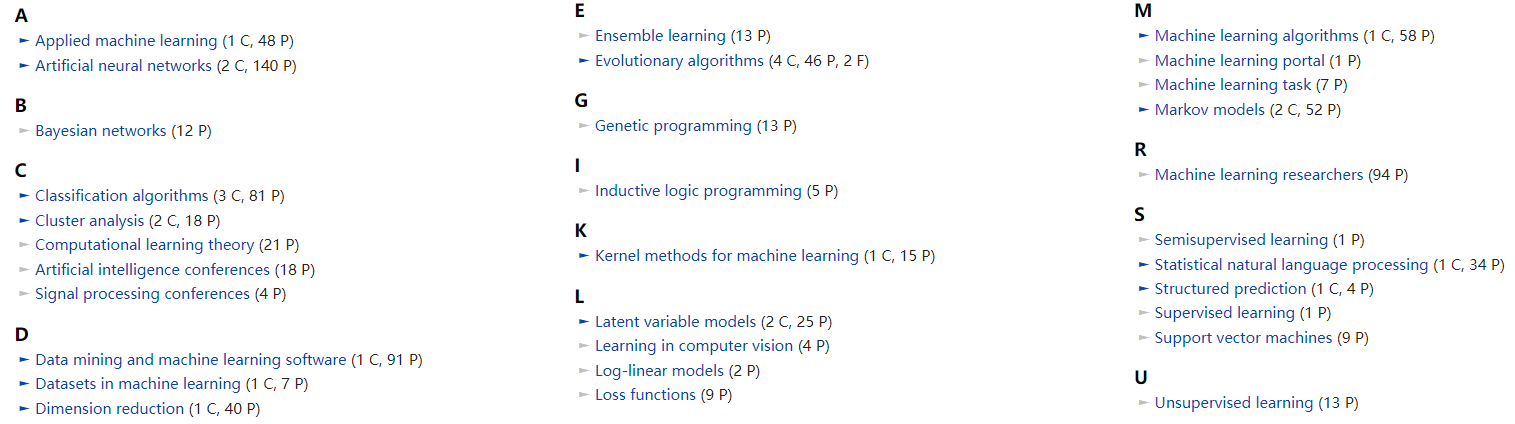
\includegraphics[width=.85\linewidth]{./figures/ml_cat.jpg}
	\caption{维基百科中Machine Learning的下位词信息}
	\label{fig:ml_cat}
\end{figure}

为说明taxonomy结构出存在的异常情况,本文给出一个三层taxonomy结构示意图,如图\ref{fig:category}所示。
\begin{figure}
	\centering
	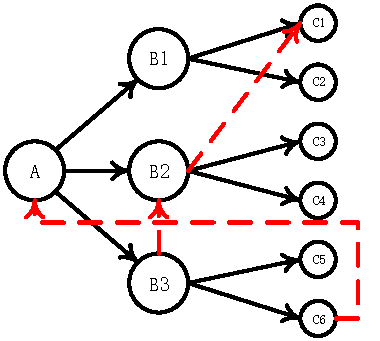
\includegraphics[width=.65\linewidth]{./figures/category.pdf}
	\caption{维基百科taxonomy层次化示意图}
	\label{fig:category}
\end{figure}

图\ref{fig:category}中红色虚线表示需要说明的情况。

\begin{enumerate}[label=\arabic*)]
	\item \textbf{B2$\rightarrow$C1}: 该路径目的是说明一个下位词可能存在多个上位词,该情况是合理的,比如一个学科可能在多个领域都有被研究。
	\item \textbf{B3$\rightarrow$B2}: 该路径说明可能兄弟之间存在上下位关系。该情况也是合理的,比如可以认为“人工智能”的两个下位词是“机器学习”和“深度学习”,而“深度学习”也可以认为是“机器学习”的下位词。
	\item \textbf{C6$\rightarrow$A}: 该路径表示出现环路,即下位词是其上位词路径上的上位词。这个显然不合理,因为上下位关系本身是一种有向关系,是一种不可逆的关系,而该路径的出现表示上下位关系可逆,因此从逻辑上讲该路径是异常的。维基百科得到的taxonomy数据存在这种关系,说明维基百科的数据在上下位关系上是存在噪声的。
\end{enumerate}


经过上述分析可知,正确上下位关系图的基本结构应为有向无环图(Directed Acyclic Graph, DAG)。

ACM CCS (Computing Classification System)分类树[8]是一个包含2126个节点的层次化实体关系,每个点可以看作一个上位词或下位词。每个非叶子节点都可作为上位词,并且在CCS分类树上存在下位词。该系统主要用于学者在ACM电子数据库中搜索符合自己需求的文献内容。同时支持将个人文章对应到CCS分类下。ACM CCS存在14个顶层分类,包括比如“Hardware”、“Network”、“Software and its engineering”等。层次深度最深达到4层。层次化数据呈现树状结构。该知识库优点是对于数据经过人工审查,分类较为仔细,缺点是只针对计算机领域,并不包括其他领域层次化数据,同时CCS发布时间是2012年,数据量过少,不包括比如“deep learning”等热门领域。因此是一个针对计算机领域的较为准确的数据库。

Microsoft Field of Study来自微软学术图(Microsoft Academic Graph, MAG)。Field of Study是微软学术图内置的一个学术上下位词关系的知识库。包含将近50000个节点,每个节点表示一个学术话题。该知识库是一个4层的有向无环图结构,每个下位词可以属于不同的上位词,MAG对这种情况给出了“可信度”这一指标,表示该下位词以多少“可信度”属于上位词。比如第3层节点“Supercomputer”是第2层节点“Operating system”的“可信度”是0.53,是第2层节点“Parallel Computing”的“可信度”是0.47。直觉上讲,超级计算机确实既会被操作系统领域研究,也会被用于并行计算研究。但是都是属于计算机领域的,因此可用Field of Study的数据得到“Supercomputer”是“Computer Science”的下位词的“可信度”是1.0。MAG的Field of Study具有严格的层次结构,它将每个节点(话题)都分成了L0至 L3这4个等级。其中L0是最高级别的上位词。统计可得各个等级的话题个数,如表\ref{tab:fos_statistics}所示。

\begin{table}[!ht]
	\centering
	\caption{MAG中Field of Study数据统计表\label{tab:fos_statistics}}
	\begin{tabular}{ccc}
		\toprule
		等级   & 个数&示例\\ \midrule
		L0 & 19 & Chemistry, Computer Science, Physics \\
		L1 & 290 & Artificial Intelligence, Organic chemistry, Algebra \\
		L2 & 1495 & Robotics, Artificial neural network, deep learning \\
		L3 & 46851 & Cognitive robotics, Logistic function, Boltzmann machine \\
		\bottomrule
	\end{tabular}
\end{table}

可以看出,L0层次的话题级别都是学科级别的话题,比如化学、计算机、物理等;L3层次的话题较为具体,一般为具体的方法等。比如logistic函数、波兹曼机等。该知识库实体个数大于ACM CCS,同时包括针对多种学科的上下位关系,不只局限于计算机领域。

以上介绍了几个常用的大规模开放可下载的知识库。同时针对本文所研究问题,介绍了3种存在上下位关系的知识库及优缺点,为了充分利用现有知识库,本文对Wiki, ACM CCS和Microsoft Field of Study进行融合,得到更大而全的上下位关系知识库。


\subsection{问题定义}

Tang等人~\upcite{tang2015sampling}从大规模社交网络中采样有代表性用户,并对问题进行了形式化定义。其中问题实例如图\ref{fig:tang_sample}所示~\upcite{tang2015sampling}。
\begin{figure}
	\centering
	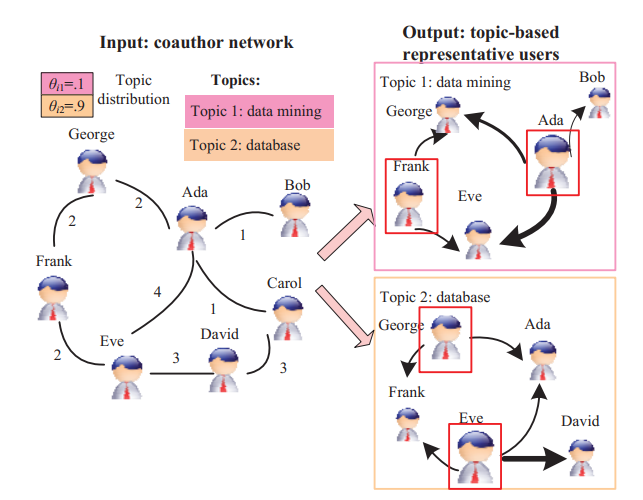
\includegraphics[width=.85\linewidth]{./figures/tang_sample.png}
	\caption{从合著者网络中采样代表性用户实例}
	\label{fig:tang_sample}
\end{figure}

对于代表性用户采样问题,给出一个社交网络$G=(V,E)$,其中$V$表示用户集合, 表示$E$有向边集合;每个用户定义有$d$个属性;希望在$V$中选出$k$个用户;将属性分为$t$组;质量函数定义为$Q$;Tang等人将如何寻找代表性用户集合$T$定义为优化问题,如式\ref{equ:tang_sample}所示:
\begin{equation}
\label{equ:tang_sample}
\setlength{\abovedisplayskip}{10pt}
\setlength{\belowdisplayskip}{10pt}
\mathop{\arg \max}_{T\subseteq V,|T=k|}{Q(G,X,\textbf{G},T)}
\end{equation}

其中$\textbf{G}$为属性组,$X$为属性的分布。$X_i$表示用户$v_i\subseteq V$的属性集合,即$X_i=[x_{ik}]_{k=1,...,d}$。

然后作者通过将问题规约为支撑集问题(Dominating Set Problem)~\upcite{garey1979guide},证明原优化问题为NP Hard问题。

\subsection{代表性话题抽取研究}

目前主要的代表性话题抽取方法包括主题模型(Topic model)、关键词抽取(Keyphrase extraction)、基于词向量的研究。

对于主题模型,可将话题看作主题模型的主题。目前主题模型已经被大量应用于抽取关键话题。Blei等人提出LDA主题模型~\upcite{blei2003latent},该模型是一种无监督学习模型,核心思想是每个文档都有多个主题混合组成,而每个单词出现在主题中的概率也不同,主题概率提供了对文档的显式表示。但是LDA模型很难给出每个分布表示的具体主题,需要通过大量人工标注。对于该问题,Mei等人提出将自动标注问题转化为最小化单词分布间的KL散度和最大化标签和主题模型的交互信息的问题。通过试验比较,发现该算法可以高效生成可解释的标签~\upcite{mei2007automatic}。Lau等人针对LDA模型提出自动标注话题的方法~\upcite{lau2011automatic}。作者利用英文维基百科数据生成标签候选集,然后利用监督学习模型SVR得出候选集标签排序,进而实现对话题的自动标注。尽管多位学者对LDA话题自动标注进行大量研究并取得一定进展,但是自动标注效果与人工标注存在明显差距。

关键词抽取技术目前主要是两种途径:监督学习和无监督学习。对于监督学习来讲,关键词抽取问题通常被看作分类问题或排序问题。Witten等人提出Kea算法用于从文本中自动抽取关键词。Kea将关键词抽取问题转化为分类问题,通过使用已知关键词的文档作为训练集,使用训练的模型找出各候选词是否属于当前文档的关键词,进而完成关键词抽取工作~\upcite{witten2005kea}。Jiang等人认为该问题类似于将候选关键词集合按特征进行排序,排名越靠前说明该关键词对于文档更重要,更可能是文档的关键词,因此作者将关键词抽取问题视为排序问题并使用learning to rank的Ranking SVM方法完成该任务,关键词抽取效果优于传统SVM和Kea算法~\upcite{jiang2009ranking}。

对于无监督学习来讲,Hasan等人将无监督方法用于解决关键词抽取问题的方法分为四组:基于图的排序法(Graph-Based Ranking)、基于主题的聚类(Topic-Based Clustering)、同时学习(Simultaneous Learning)、语言模型(Language Modeling)~~\upcite{hasan2014automatic}。

基于图的排序法最有代表性的是Kleinberg等人提出的HITS算法~\upcite{kleinberg1999authoritative}和Google提出的PageRank算法~\upcite{brin1998anatomy}。Mihalcea等人提出TextRank算法用于自动关键词抽取~\upcite{mihalcea2004textrank},将文本看成图,将本文分词,并进行词性标注,用点表示关键词,边表示关键词之间的共现关系构成图。基于PageRank算法思想,迭代计算各节点权重,直到收敛。根据迭代结果找出最重要的 个单词,即为关键词。

基于主题的聚类法是将关键词分成多个主题组,直觉上每个抽取出来的关键词应该包含文章中的所有主要主题。Liu等人利用聚类技术找出代表性术语,将每个类的代表性属于作为种子自动抽取关键词。研究表明大部分人工选取的关键词都是名词,因此作者对文档进行词性标注,主要抽取其中的名词和形容词。实验表明准确率在F1值上超过TextRank 9.5\%~\upcite{liu2009clustering}。Hasan等人指出基于关键词聚类的方法为所有主题分配相同的重要性,实际文档中有些话题并不主要~\upcite{hasan2014automatic},因此可能存在缺陷。

同时学习是基于一个假设:重要的词出现在重要的句子中,重要的句子包含重要的词。因此文本摘要和关键词抽取同时学习可能能共同提高效果~\upcite{zha2002generic}。Wan等人进一步做出两点假设:1)关键句与其他关键句相连;2)关键词与其他关键词相连~\upcite{wan2007towards}。基于上述假设,Wan等人寄建立三个捕获句子(S)和单词(W)间关系的图:S-S图、S-W图和W-W图。S-S图的边权重表示两个句子的相似度;S-W图的边权重表示词在句子中的重要性;W-W图的边权重表示两个单词之间的共现次数或者基于知识的相似度。最后通过迭代强化算法为每个句子和单词分配权重,权重高的单词作为关键词~\upcite{wan2007towards}。

语言模型通过两个特征评价关键词:词组性(Phraseness)和信息性(Informativeness)~\upcite{tomokiyo2003language}。词组性表示单词序列是否可看作词组;信息性表示哪个单词捕获了文档的中心含义。直觉上讲,有高词组性和信息性的词组更可能是关键词。Tomokiyo等人通过语言模型分别在前景语料库(Foreground corpus)和背景语料库(Background corpus)上训练得到这两个特征。前景语料库由存在关键词的文档组成,背景语料库是来自Web的大量无标注文本数据。通过语言模型得到特征值之后按照两者加和排序候选关键词~\upcite{tomokiyo2003language}。

词向量(Word Embedding)将单词特征进行稠密编码,将特征映射到隐特征空间。Mikolov等人提出通过预测单词和上下文单词来获取低维特征表示的Word2Vec方法~\upcite{mikolov2013distributed}。Word2Vec的主要包括两种算法:Skip-gram(SG)和连续词袋模型(Continuous Bag of Words, CBOW)。SG算法是通过当前单词预测上下文单词,CBOW是通过上下文单词的词袋模型预测目标单词。训练时为了更加高效可以使用两种算法:层次化Softmax(Hierarchical Softmax)和负采样(Negative Sampling)。因为本文研究是基于词向量相似度的代表性话题抽取,因此下面重点介绍Skip-gram模型的工作流程。

Skip-gram模型通过当前单词预测周围单词出现的概率。如图\ref{fig:skip_gram_model}所示~\upcite{mikolov2013distributed}。
\begin{figure}
	\centering
	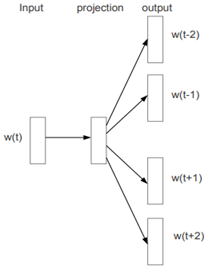
\includegraphics[width=.45\linewidth]{./figures/skip_gram_model.png}
	\caption{Skip-gram模型结构}
	\label{fig:skip_gram_model}
\end{figure}

Skip-gram通过单隐层神经网络完成预测周围单词出现概率的任务。但这实际是一个“伪任务”~\upcite{mccormick2016word2vec}。即真正想要的并不会真正使用模型去完成上述预测任务,而是为了得到隐层权重,因此实际“伪任务”得到的权重就是通过Skip-gram模型得到的词向量。

输出的概率表示每个单词更有可能在输入单词附近的概率。比如给出输入单词“Soviet”,周围的单词是“Union”或者“Russia”的概率较大,而是“西瓜”或者“袋鼠”的概率就很小~\upcite{mccormick2016word2vec}。而在输入单词附近由“窗口大小”衡量。比如存在句子“The quick brown fox jumps over the lazy dog.”,假设窗口大小$c=2$。表示在中心词前后各选择两个单词作为环境词。最终得到训练样本<输入,输出>为:<the, quick>, <the, brown>, <quick, the>, <quick, brown>, <quick, fox>, <brown, the>, <brown, quick>, <brown, fox>, <brown, jumps>, <fox, quick>, <fox, brown>……后面模式相同。通过训练,即可通过训练好的模型预测当前单词周围的词汇出现的概率。

更一般地,给出句子序列$S=<w_1,w_2,...,w_T>$,其中$T$为序列长度。利用最大似然估计可得,Skip-gram的目标是最大化式:
\begin{equation}
\label{equ:skip_gram_target}
\setlength{\abovedisplayskip}{10pt}
\setlength{\belowdisplayskip}{10pt}
J(\theta)=-\frac{1}{T}\sum_{t=1}^{T}\sum_{-c\leq j\leq c, j\neq 0}\log p(w_{t+j}|w_t)
\end{equation}

其中$c$是训练窗口大小,$c$越大训练数据越多,准确率也越高,但是耗费时间也越大。式\ref{equ:skip_gram_target}中的$p(w_{t+j}|w_t)$使用了softmax函数表示,如式\ref{equ:skip_gram_p}所示。
\begin{equation}
\label{equ:skip_gram_p}
\setlength{\abovedisplayskip}{10pt}
\setlength{\belowdisplayskip}{10pt}
p(w_O|w_I)=\frac{\exp ({v'_{wO}}^{T}v_{wI})}{\sum_{w=1}^{W} \exp ({v'_w}^{T}v_{wI})}
\end{equation}

其中$v_w$和$v'_w$分别表示单词$w$的输入、输出向量表示。$W$表示词表大小。

实际该模型可以展示为一个三层的神经网络。其中隐含层为线性激活单元,输出层为Softmax分类器。具体结构如图\ref{fig:skip_gram_structure}所示~\upcite{mccormick2016word2vec}。
\begin{figure}
	\centering
	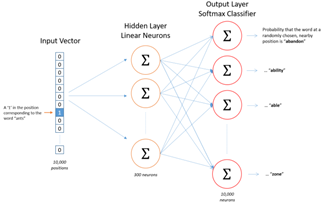
\includegraphics[width=.65\linewidth]{./figures/skip_gram_structure.jpg}
	\caption{Skip-gram网络结构示意图}
	\label{fig:skip_gram_structure}
\end{figure}

输入层到隐含层的参数$W$维度为$|V|\times |H|$,即词表大小乘以隐含层大小。$w(i,:)$可以看作第$i$个单词的词向量。如果两个不同的单词有相似的上下文,即出现在其周围的单词较为相似,则Skip-gram模型将输出相似的结果。因此如果两个单词上下文相似,则模型倾向于学习相似的词向量。

因此可知,词意相似的单词词向量也比较相似,而可以认为下位词的词向量应与上位词词向量相似,进而实现代表性话题抽取。尽管存在Glove等更优秀的单词分布式表示方法~\upcite{pennington2014glove},但是由于效率和易用性等原因,还是考虑使用Skip-gram。

\subsection{强化学习在NLP领域的应用}

近年来,强化学习(Reinforcement Learning)与深度学习结合,开始成为研究热点问题~\upcite{mnih2013playing}。因此强化学习也在各领域大放异彩。2015年10月AlphaGo击败欧洲围棋冠军,2016年3月击败18次获得世界围棋比赛冠军的李世石,2017年5月击败围棋世界第一柯洁。并且提出完全自我训练的AlphaGo~\upcite{silver2016mastering}。2017年12月,Deep Mind团队公开AlphaZero~\upcite{silver2017mastering},同时在多种棋类上做出大量提升。这是强化学习最引人注目的应用之一~\upcite{silver2016alphago}。下面本文先简单介绍强化学习的基本知识和核心概念,然后介绍近年来强化学习在NLP领域的应用。

强化学习是Agent与环境(Environment)交互的过程,通过学习最优策略(Policy)和试错(Trail and error)解决序列决策问题(Sequential decision making problem)。强化学习问题在于学习做什么才能最大化所得奖赏(Reward),即如何将当前状态(State)映射为动作(Action)。本质上强化学习问题是一个闭环问题(Closed-loop),因为学习系统的行为会影响下一次的输入~\upcite{sutton1998reinforcement}。强化学习过程示意图如图\ref{fig:rl_interaction}所示\footnote{goo.gl/UqaxlO}。

\begin{figure}
	\centering
	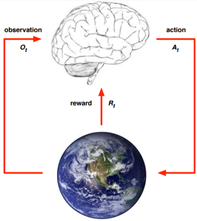
\includegraphics[width=.65\linewidth]{./figures/rl_interaction.png}
	\caption{强化学习Agent和Environment交互过程}
	\label{fig:rl_interaction}
\end{figure}

图\ref{fig:rl_interaction}展示了强化学习的交互过程,其中,在第$t$步,agent执行动作$A_t$,收到观测$O_t$等价于上文所述的State$S_t$),收到标量奖赏$R_t$。环境收到动作$A_t$,发出观测$O_{t+1}$(等价于$S_{t+1}$),发出标量奖赏$R_{t+1}$。$t$在每次交互完成后递增。

定义当前时刻$t$的累计奖赏为:
\begin{equation}
\label{equ:rl_reward}
\setlength{\abovedisplayskip}{10pt}
\setlength{\belowdisplayskip}{10pt}
R_t=\sum_{k=0}^{\infty} \gamma^kr_{t+k}
\end{equation}
其中$\gamma\in(0,1]$为折扣因子(discount factor),$r_t$表示$t$时刻的即时奖赏。

价值函数(Value Function)用于衡量当前状态的好坏程度,可用累计奖赏的期望表示。即:
\begin{equation}
\label{equ:rl_value_function}
\setlength{\abovedisplayskip}{10pt}
\setlength{\belowdisplayskip}{10pt}
v_\pi(s)=E[R_t|s_t=s]
\end{equation}
其中$v_\pi(s)$为在状态$s$下使用策略$\pi$的期望累积奖赏值。将$v_\pi(s)$分解为Bellman等式可得:
\begin{equation}
\label{equ:rl_bellman}
\setlength{\abovedisplayskip}{10pt}
\setlength{\belowdisplayskip}{10pt}
v_\pi(s)=\sum_a \pi(a|s)\sum_{s',r}p(s',r|s,a)[r+\gamma v_\pi(s')]
\end{equation}

最优状态值可定义为:
\begin{equation}
\label{equ:rl_optimal}
\setlength{\abovedisplayskip}{10pt}
\setlength{\belowdisplayskip}{10pt}
v_*(s)=\max_\pi v_\pi (s)=\max_a q_{\pi *}(s,a)
\end{equation}

若强化学习问题满足Markov性质,即下一步状态只依赖于当前状态和动作,与过去无关,则可以将问题看作Markov决策过程(Markov Decesion Process, MDP),用五元组$(S,A,P,R,\gamma)$表示~\upcite{li2017deep}。对于有模型学习(Model-based learning)问题,机器已对环境进行建模,状态、动作、状态转移概率、转移奖赏函数均为已知,则可考虑使用动态规划方法:策略评估(Policy evaluation)计算策略的价值函数,策略迭代(Policy iteration)或值迭代(Value iteration)找到最优策略。对于免模型学习(Model-free learning)问题,环境转移概率、奖赏函数、甚至不知道环境中一共有多少状态。此时可以使用蒙特卡洛方法,根据执行该策略$T$步得到的采样轨迹$<s_0,a_0,r_1,s_1,a_1,...,s_{T-1},a_{T-1},r_T,s_T>$可得到状态-动作值函数的估计。另一种解决方法是时序差分学习(Temporal Difference, TD),同时利用采样轨迹和动态规划结构,得到值函数或状态-动作值函数的估计。SARSA算法~\upcite{rummery1994line}和Q-Learning算法~\upcite{watkins1992q}是经典的TD learning算法~\upcite{arulkumaran2017brief}。

之前提到的值函数或状态-动作值函数均被以表格形式存储,但是当状态空间很大或者连续时,内存需求会太大甚至无法存储,因此需要使用近似值函数(Function Approximation)估计值函数。这种近似函数可以是线性函数或非线性函数,DQN则通过使用CNN实现端到端的强化学习~\cite{mnih2013playing,mnih2015human},实现直接从像素输入学习游戏打法并超过顶尖人类玩家水平。

除了TD learning和Q-learning等基于值的方法(Value-based methods),还有基于策略的方法(Policy-based methods)。基于策略的方法目标是直接优化策略$\pi(a|s;\theta)$,其中$\theta$是近似函数的参数,并通过梯度上升(Gradient ascent)方法优化$E[R_t]$。Williams等人提出的REINFORCE算法是一种经典策略梯度(Policy gradient)算法,在方向$\nabla_\theta \log \pi(a_t|s_t;\theta)$上更新参数$\theta$。

强化学习在多个NLP子领域开始被应用,包括对话系统(Dialogue system)、机器翻译(Machine translation)、文本生成(Text generation)~\cite{li2017deep,williams1992simple}。在对话系统领域,Li等人基于监督学习和强化学习提出端到端的神经对话系统。该框架包括用户仿真器和神经对话系统。作者利用强化学习端到端的训练系统,将对话策略看作DQN,进而降低其他模块产生的噪声~\cite{li2017end}。在机器翻译领域,He等人提出对偶学习处理机器翻译领域数据不足的问题。机器翻译从语言A到语言B和对偶任务,从语言B到语言A,可以帮助提高两个翻译模型性能。作者使用策略梯度方法,使用语言模型似然度作为奖励函数。实验表明该模型只需要较少数据即可实现优越性能~\cite{he2016dual}。文本生成是多种NLP任务的基础,比如对话生成、机器翻译、自动摘要等。Bahdanau等人使用强化学习算法actor-critic实现序列预测,使用critic网络预测单词的价值,即actor网络定义的序列预测策略的期望累计价值~\cite{bahdanau2016actor}。除此之外,强化学习开始被用于微调(Fine-tuning)模型结果。Zhang等人使用RNN decoder和attention机制对病人病症生成治疗药物,保证药物之间不出现药物冲突。使用策略梯度方法基于规则去除仍存在冲突的药物组合,实验表明强化学习可以实现机制冲突药物组合的产生~\cite{zhang2017leap}。


\section{论文研究内容}
在历史文献当中,源词和目标词分别被称为模型的输入和输出。源词通常可以用分布式表示(Distributed Representation)来表示,称为输入词嵌入(Word Embedding),通常在大规模语料上使用连续词袋模型(CBoW)、跳跃单词模型(Skipgram)或者~Fasttext~模型来训练。
而这几种模型均起源于语言建模任务,并且考虑到实际运算的效率而去除了部分冗余结构。
另外,输出端的词表通常表示为单词索引(Indexing)或~$1-K$~编码,并且可以与~softmax~概率函数直接关联。

在语言模型研究领域中,大词表问题是目前理论应用到实际过程中必须要克服的问题,我们当然可以通过配置高性能服务器来缓解该计算瓶颈。一旦应用到较大规模的数据集上,即使是目前最好的中央处理器(CPU)或者通用计算图形处理器(GPGPU),仍然需要数周时间才能训练完善。因此,在保证原有模型的准确率和精度的前提下,如何提高模型的训练速度是本文主要讨论和研究的内容。为此我们考察了两个主要的研究目标:上下文信息建模效率和精度对比、大词表问题的优化和研究。

针对大词表问题的优化,目前主要采用的方案有以下几种:一种是采用子词(Subword-level)或者字符级别的词(Character-level)来直接缩小词表大小;一种是通过采样技术(Sampling-based Approximation)来减少必要的训练时间;另一种是通过基于分类的多元分类(class-based Hierarchical Softmax,cHSM)和采用基于树模型的多层二元分类模型(tree-based Hierarchical Softmax,tHSM)来加速模型。

本论文考虑了层次概率模型所存在的一些问题,并提出相应的解决策略。首先,我们提出了一个在分层结构上建模参数的单词编码方案,推导出紧凑的代价函数及其梯度。同时考虑到类或树上的单词分布对其性能有很大的影响,我们运用文本的统计,句法和语义知识来初始化其参差结构,以达到稳定的计算精度。同时在推理过程中,我们考虑了两种不同的推理情况:句子打分和文本排序,并提出了对应的优化策略。
\section{论文的组织结构}
\textbf{第一章:}``绪论'',主要介绍了本论文的研究背景和意义,另外简要说明了语言模型的发展历史以及本文的主要工作,并对本文的组织架构进行了说明。

\textbf{第二章:}``相关技术介绍'',对历史上的各个学术分支在语言模型的任务上的相关工作进行了介绍。

\textbf{第三章:}``树状层次概率模型'',介绍了基于二叉树的层次概率模型,并与传统树状模型做了理论层面的比较。同时还研究了在推理测试阶段,二叉树层次概率模型应用的贪心策略,以保证实际测试结果性能和效率。

\textbf{第四章:}``类别层次概率模型'',介绍基于分类的层次概率模型,并分析了词表非均匀划分所产生的后果,进而探讨了类别不均匀问题所带来的影响以及相关解决策略。最后探讨了在测试阶段,语言模型的任务需求和分类层次概率模型相应的解决算法。

\textbf{第五章:}``语言建模实验及结果分析'',实证研究了本论文提出的层次概率模型的实际效果,并和其他算法在各个指标维度上进行了比较和分析。

最后结论部分,总结了全论文的贡献和工作,并提出了未来的工作方向,同时撰写了结束语。




%\chapter{相关技术介绍}
在自然语言处理研究领域中,基于神经网络的分布式表示(Distributional Representation)通常被称作为词向量(Word Vector)、词嵌入(Word Embedding)或者分布式表示(Distributed Representation)~\upcite{DBLP:conf/nips/MikolovSCCD13}。基于神经网络的词向量表示技术是通过对语言模型的两个组成部分进行建模,即:1)单词的语境,也称为上下文(Context);2)以及上下文与下一步的目标单词之间的关系(Next-Utterance Prediction)。
神经网络结构和组合方式相对灵活,可以表示更加复杂的上下文语义结构(Complex Context)。
历史上的词向量表示方法主要是基于单词共现矩阵(Co-occurrence Matrix),仅仅是利用了单词的顺序信息。
单词的语义向量是通过将单词共现矩阵进行矩阵分解(Matrix Decomposition),例如奇异值分解算法(Singular Value Decomposition,SVD)、潜在语义分析模型(Latent Semantic Analysis,LSA)或者潜在语义索引(Latent Semantic Indexing,LSI)等分解算法。其中对于SVD分解算法,第一个分解获得的矩阵就是我们需要的单词的词向量矩阵。
N-gram~算法也是使用单词的顺序信息作为上下文信息建模策略,当~$N$~线性增加时,N-gram~模型所需要存储的单词序列组合总数会呈指数爆炸增加,即维数灾难问题(Curse of Dimensionality)\footnote{https://en.wikipedia.org/wiki/Curse\_of\_dimensionality},它深深限制了~N-gram~模型的实际应用。
假若使用神经网络替代~N-gram~模型来表示单词概率分布,当~$N$~线性增加时神经网络语言模型所需要的参数数量仅以线性速度增长。
这样我们就可以利用神经网络模型可以对更复杂的文本结构进行建模,在从训练后的模型获得的词向量中,将包含更多的语义信息、结构知识。

到目前为止,在语言模型的领域中,研究者提出的神经网络模型主要包括: 传统前向传递神经网络(Feed Forward Neural Network, FFNN)、循环神经网络(Recurrent Neural Network, RNN)三种基本的建模方案。当然基于这些基本组件,我们还可以构造更复杂的模型结构,但是无法保证复杂模型一定在效率和精确度上优于简洁的模型结构。复杂的模型可以表征更复杂的本文语义信息,例如句子的依存关系(Dependency)结构或者句子的句法分析树(Syntactic Structure)结构,但是这样的效果不一定能保证模型的泛化性能(Generalization)会很好,因为日常文本的语序是存在较多混乱的数据,很难找到良好定义的句子关系,所以也无法让模型从混乱的文本分布中学习到有效的句子结构,以提升模型的精度。显然是假设越弱模型越好,因为针对复杂的网络文本数据,我们模型训练所需要的数据质量相对较低,模型越容易收敛并获得有效的结果。模型假设越强,模型所需要的数据质量越高,实际稳定性就会降低,产生得不偿失的后果。


除此以外,针对在本论文所讨论的语言模型的大规模应用过程中所遇到的大词表问题,历史文献中提出的解决方法主要可以划分为:单词拆分算法(Vocabulary Truncation)、采样估计模型(Sampling-based Approximation)和词表层次分解(Vocabulary Factorisation),我们会在接下来的章节陆续介绍。其中本论文重点是研究基于类别的多元分类模型(class-based hierarchical softmax, cHSM)和基于二叉树的二元分类模型(class-based hierarchical softmax,tHSM),这两种算法将在下一章更详细讨论和介绍。

\section{语言建模}
在这一节中,我们将首先从语言模型提出的实际背景的形式化定义开始,以阐述语言模型的训练目标和实际应用场景~\upcite{DBLP:journals/tnn/ChienK16}。一个好的语言模型应当考虑对文本的两种特征进行建模:语法特征(Syntactics)和语义特征(Semantics)。为了保证句子的语法正确,我们需要考虑的是所生成的单词的前面的上下文(Previous Context),这也就意味着语法特性往往只对局部特征(Local Representation)进行建模。而语义特征的一致性则复杂了许多,它意味着我们需要考虑更大、更完善的上下文信息乃至整个文档语料,来获取全局语义(Global Context)而不仅仅是局部语义信息(Local Context)。


具体地来说,给定一个包含$T$个单词的序列:$w_1,w_2,\cdots,w_T$,这个序列的概率或者对数概率(Log-probability),即描述该序列作为一个合理且合法的句子的流畅性(Fluency)和出现该单词组合的句子的可能性( Likelihood)。由于直接求解整个序列的概率比较复杂,所以我们将采用马尔可夫链规则(Markov Chain)~\footnote{https://en.wikipedia.org/wiki/Markov\_chain},分解成一系列的条件概率(Conditional Probability)的联合分布(Joint Distribution):
\begin{equation}\label{laguage_model}
\setlength{\abovedisplayskip}{10pt}
\setlength{\belowdisplayskip}{10pt}
 \log p(w_1,\cdots, w_T ) = \sum_{t=1}^T \log p(w_t | w_{1:t-1}),
\end{equation}
其中前 $t-1$个单词记作$w_ {1:t-1}$。进而,条件概率~$p(w_t | w_ {1:t-1})$表示给定其前面上下文$w_ {1:t-1} $作为预测的下一个单词的条件概率分布(Conditional Probability)。最早的传统方法可以由前馈网络来建模这个上下文信息, 同时用 softmax 函数来表示下一个单词的概率分布计算公式~\upcite{DBLP:journals/jmlr/BengioDVJ03}。 在训练的过程中,整个模型以最小化每个单词预测的交叉熵损失(Cross Entropy Loss)为目标:
\begin{equation}\label{equ:losses2}
\setlength{\abovedisplayskip}{10pt}
\setlength{\belowdisplayskip}{10pt}
  \ell=\sum_{t=1}^{T}\ell_t=\sum_{t=1}^{T}\log p(w_t | w_{1:t-1})
\end{equation}
其中文本或者句子的交叉熵代价函数$\ell$ 的实际意义为:是当编码方案不一定完美时,平均编码长度是多少(最优的编码长度就是1)。这里的编码长度的概念可以理解为:如何用01字节对所有的单词进行最短的编码,保证单词之间两两不互相冲突。交叉熵代价函数是由$\texttt{KL}$散度(Kullback–Leibler Divergence),也叫做相对熵(Relative Entropy),推导而获得的。这里我们需要注意的是,$\mathtt{KL}$散度的计算公式是:
\begin{equation}\label{equ:losses}
\setlength{\abovedisplayskip}{10pt}
\setlength{\belowdisplayskip}{10pt}
  \mathtt{KL}(p||q)=-\sum_{t=1}^{T}p(x)\log q(x) - (\sum_{t=1}^{T}p(x)\log p(x))
\end{equation}
其中$p(x)$ 指的是文本数据的真实概率分布,$q(x)$ 是由模型从数据中计算得到的预测概率分布。由于$p(x)$ 和$q(x)$ 在公式中的地位不是相等的,所以$\texttt{KL} (p\parallel q)\not\equiv \texttt{KL}(q\parallel p)$。对于给定的文本语料训练数据集,第二项的计算值是常数,由此可知其导数是0,它不会对模型中的参数更新产生任何影响。所以在通常情况下,我们采用交叉熵函数$\ell$作为模型的代价函数而不是相对熵代价函数$\mathtt{KL}$,但其实我们希望模型优化的目标是$\mathtt{KL}$使得模型的分布拟合实际的分布。
\subsection{语言模型的应用}
语言模型的实际用途包括分词(Word Segmentation或Word Breaker,WB), 信息抽取(Information Extraction,IE), 关系抽取(Relation Extraction,RE), 命名实体识别(Named Entity Recognition,NER), 词性标注(Part Of Speech Tagging,POS), 指代消解(Coreference Resolution), 句法分析(Parsing), 词义消歧(Word Sense Disambiguation,WSD), 语音识别(Speech Recognition), 语音合成(Text To Speech,TTS), 机器翻译(Machine Translation,MT), 自动文摘(Automatic Summarization), 问答系统(Question Answering), 自然语言理解(Natural Language Understanding), 光学字符识别(Optical Character Recognition,OCR), 信息检索(Information Retrieval,IR)\upcite{DBLP:journals/jair/GattK18}。

当我们对这些纷繁复杂的应用作一定抽象之后,可以将语言模型的主要作用分为以下三种情况:1) 为句子打分(Sentence Scoring)。给定一个未知的单词序列,我们需要计算其作为一个句子的流畅性和出现的可能性;2) 挑选最佳的候选词(Next-utterance Prediction)。给定上下文,选择概率最高的单词。这里所指的上下文的形式是广义的,它可能是:前面的句子给定,选择下一个最佳单词;前面和后面的句子给出,选择中间最适配的单词;后面的句子给定,选择上一个最佳单词(逆序文本建模也是有其独特应用地位的);3) 训练词向量(Pretrained Word Embedding)。语言模型的输入,在经过大规模数据集训练之后,可以作为词向量输出,从而为其他文本任务提供有效的单词预训练特征。

\subsection{长距离依赖}
不同于前馈神经网络语言模型,循环神经网络语言模型使用隐藏层状态(Hidden State)来记录单词的顺序性信息(Sequence Order),它能够捕捉句子中存在的长距离依赖关系(Long-term Dependency)。这里的长距离依赖主要指语义对应关系(Semantic Correspondence)和选择限制(Selectional Preferences)\upcite{贾玉祥2014汉语语义选择限制知识的自动获取研究}。

一方面,两个单词距离较远但是 在文本中会存在很强的相关性关系。这里的所指的相关性,包括两个单词具有语义对应关系,或者他们需要满足句子的语法结构(Grammatical Structure)。如果采用传统的~N-gram~建模策略,我们必须要建模N-gram($N>3$)单词概率分布,才能保证模型能学习到这种对应关系。

\begin{figure}[!b]
  \centering
  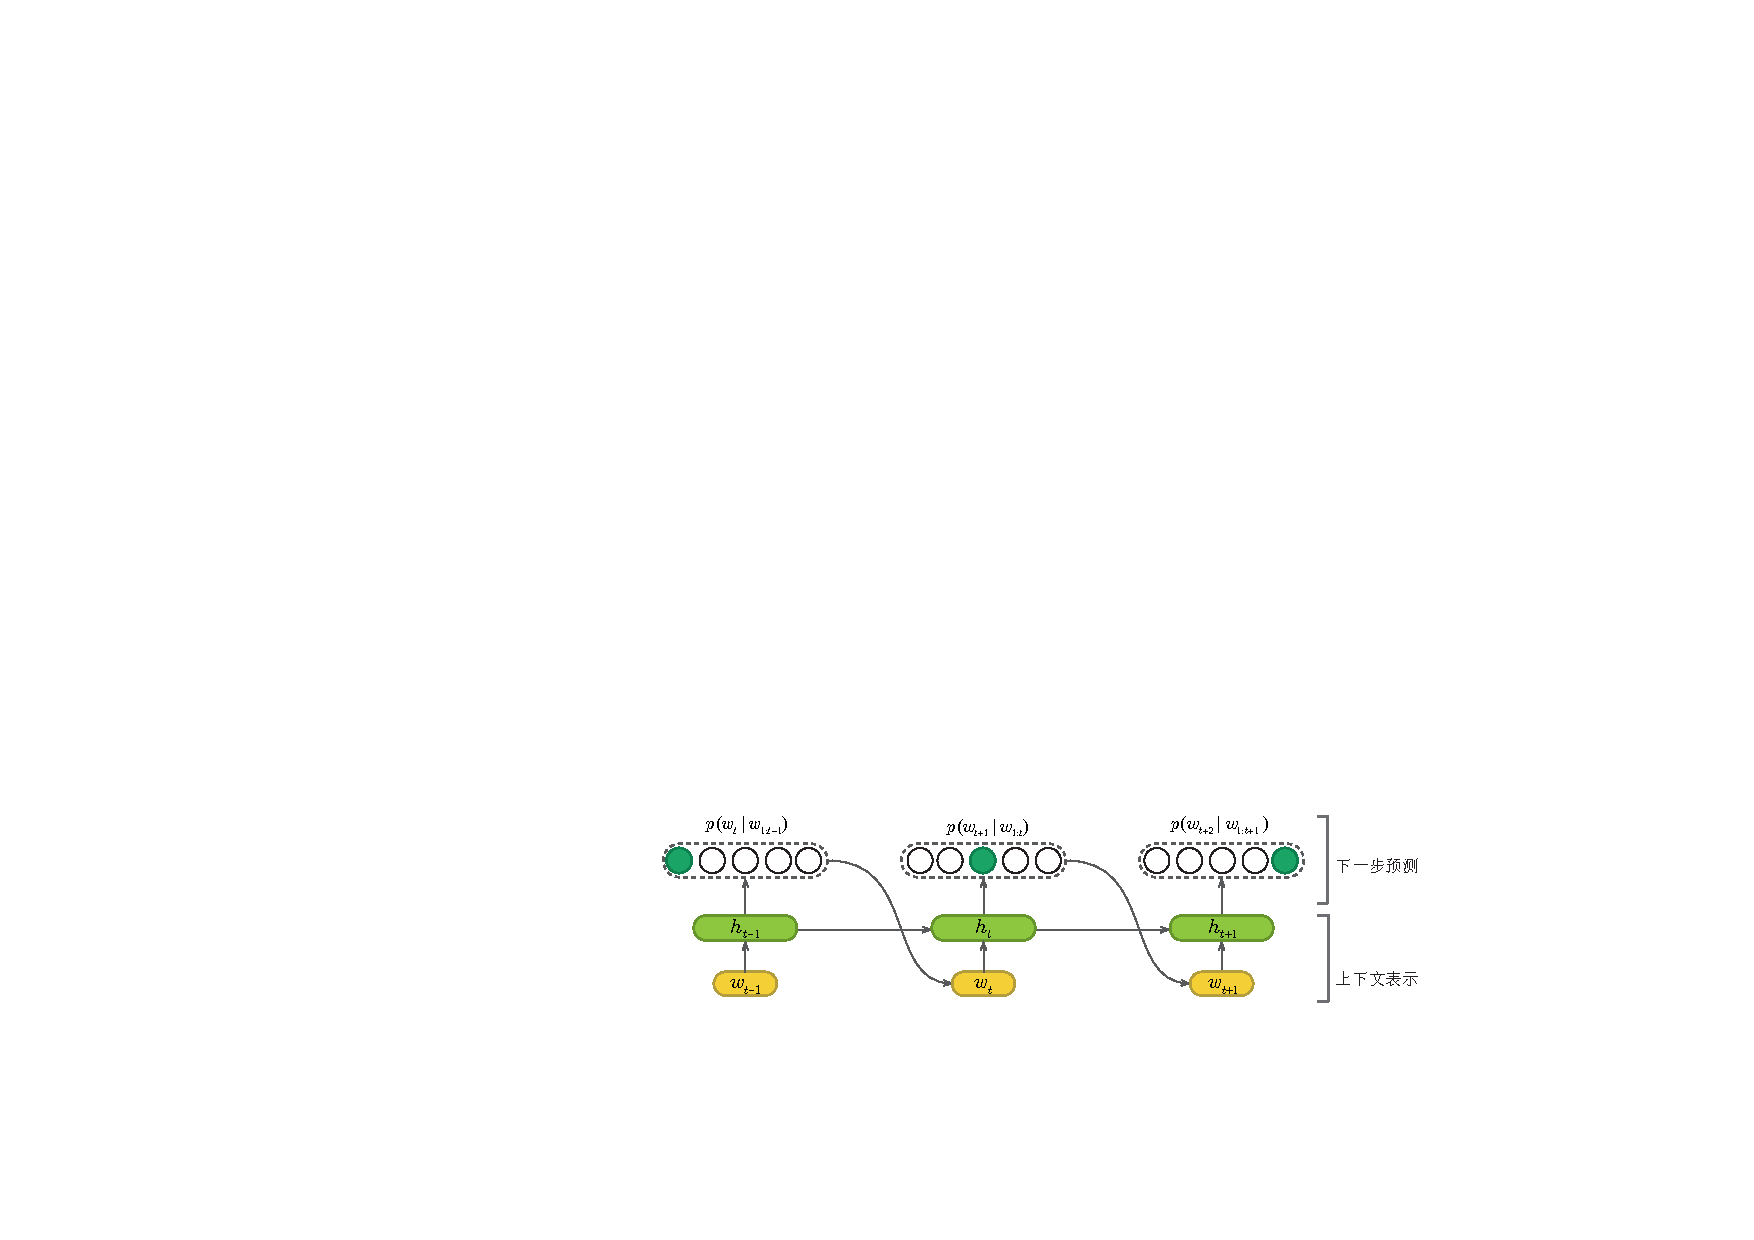
\includegraphics[width=.99\columnwidth]{./figures/lm.pdf}
  \caption{循环神经网络语言模型图例}
  \label{fig:lm}
\end{figure}

另一方面,文本中存在的依赖关系将会限制我们选择接下来的单词候选集,称其为选择限制关系。
如图~\ref{fig:lm}~所示,模型在预测过程中,在每一步都需要对词表中所有单词做预测,我们需要将每一步都做选择限制,减少模型的预测分支,这样才能保证模型生成的结果尽可能的语义一致且连贯。每次开放式的对所有单词做预测所带来的后果可能是,那些高频单词会不断出现在预测序列里面,因为训练语聊里面这些单词出现频率就非常高,所以模型将这些高频词预测概率大也是合乎情理的。但问题出现在,一旦我们模型不断预测高频词,我们生成的句子很难传达有效的语义信息。

\subsection{循环神经网络}
考虑到上面描述长距离依赖问题,在本实验中,我们将采用的基准模型是循环神经网络语言模型。近年来,基于时间序列建模的循环神经网络已经非常流行。如图~\ref{fig:lm}~所示,由于在当前时间步 $t$的输出$w_{t+1}$正好是下一个时间步的输入$w_{t+1}$,所以将上一步的输出接到下一步的输入。当我们需要做文本生成时,才需要利用这样的自循环链接(Auto-associative Connection)。每个句子都需要用开始词(即,$\langle s\rangle$)和结束词(即$\langle / s\rangle$)标记进行封装。 在预测下一个单词 $\hat w_{t+1}$ 之前,需要用到前一时刻的隐藏状态$h_{t-1}$和当前读入的单词~$w_t$~来计算网络单元的输入$h_t$。
\begin{equation}
\setlength{\abovedisplayskip}{10pt}
\setlength{\belowdisplayskip}{10pt}
  \hat w_{t+1}=\arg\max_{w\in\mathcal{V}} \mathtt{softmax}(Vh_t+d)
\end{equation}
从形式上讲,循环神经网络是一个参数化的非线性函数$\phi(w_t,h_{t-1})$,循环地将一系列向量映射到一系列隐藏状态。 将$\phi(w_t,h_{t-1})$函数应用于任何这样的序列,在每个时间步骤$t$产生隐藏状态$h_t$,如下所示:
\begin{equation}
\setlength{\abovedisplayskip}{10pt}
\setlength{\belowdisplayskip}{10pt}
  h_t \leftarrow  \phi(W\theta^w_t + U h_{t-1} +c),
\end{equation}
其中$ W,U,V $是模型参数,向量~$\theta^w_t$~对应于源词~$w_t$~的词向量。参数~$U$~是随时间共享的,即:当我们需要计算 $h_t$,我们需要用到上一步的隐藏层的输出$h_{t-1}$。

自Elman提出基本结构~\upcite{DBLP:journals/cogsci/Elman90}~以来,许多扩展模型能学习长距离依赖关系,解决梯度消失(Gradient Vanishing)和梯度爆炸(Gradient Exploding)等问题, 如长短期记忆网络(LSTM)\upcite{7508408}、门限记忆单元(GRU)\upcite{DBLP:conf/nips/ChungKDGCB15}和近似递归神经网络(Quasi-RNNs)\upcite{DBLP:journals/corr/BradburyMXS16}。

\begin{figure}[!t]
  \centering
  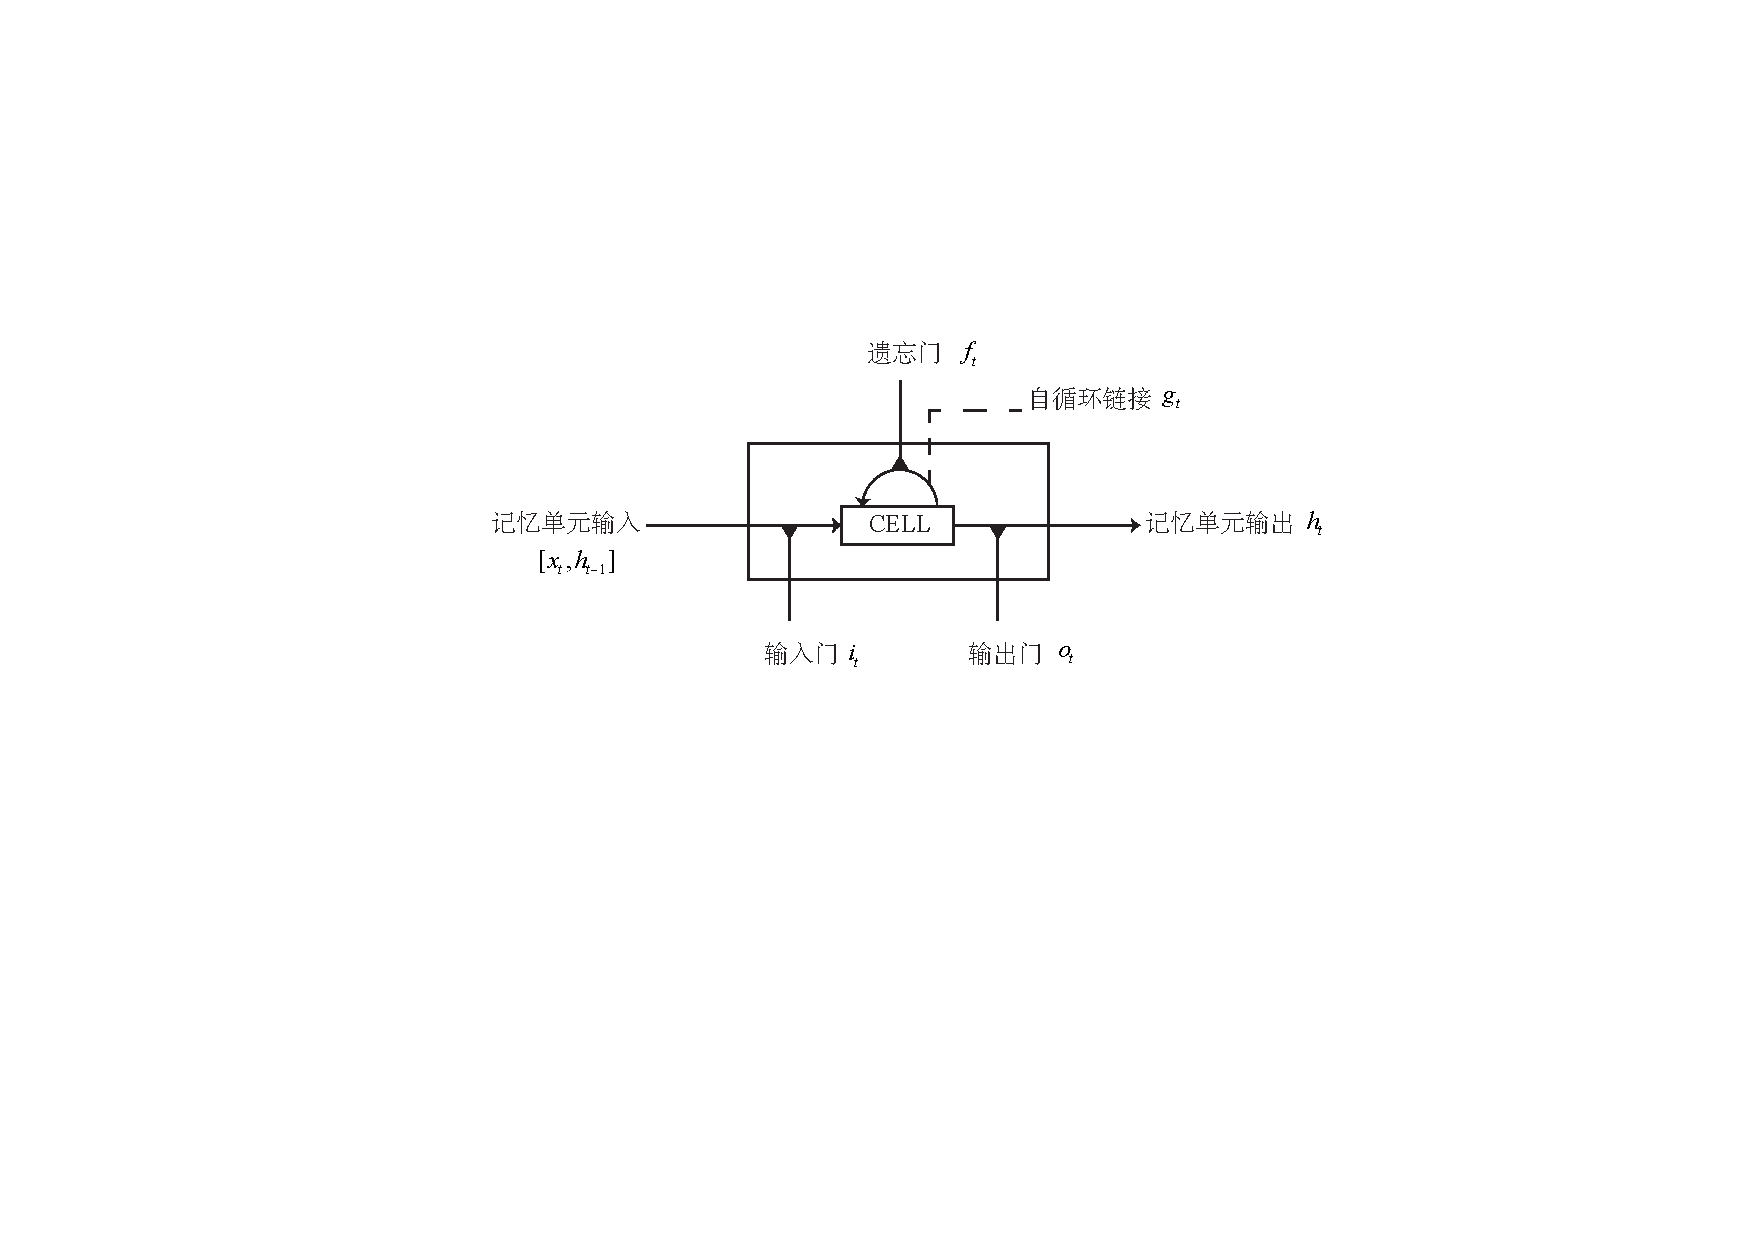
\includegraphics[width=.8\linewidth]{./figures/lstm.pdf}
  \caption{LSTM 模型示意图}\label{fig:lstm}
\end{figure}

长短记忆网络(LSTM)是根据RNN 所改进的最著名的模型之一,LSTM 模型的计算公式定义如下\upcite{DBLP:journals/neco/HochreiterS97}: 1)输入门$i_t$ 控制当前输入 $x_t$ 和前一步输出 $h_{t−1}$ 进入新的 Cell 的信息量;2) 遗忘门$f_t$ 决定是否清除或者保持单一部分的状态;3) 变换输出和前一状态到最新状态~$g_t$;4) 输出门$o_t$计算 Cell 的输出 ;5) cell 状态更新$s_t$。其计算步骤是,计算下一个时间戳的状态使用经过门处理的前一状态和输入;6) 最终 LSTM 的输出$h_t$ 使用一个对当前状态进行 $\tanh$ 变换。其计算公式如下:
\begin{equation}\label{equ:lstm}
\setlength{\abovedisplayskip}{10pt}
\setlength{\belowdisplayskip}{10pt}
\begin{split}
   i_t&=\sigma(W^i x_t+U^i h_{t-1}+b^i) \\
   f_t&=\sigma(W^f x_t+U^f h_{t-1}+b^f) \\
   g_t&=\phi(W^g x_t+U^g h_{t-1}+b^g) \\
   o_t&=\sigma(W^o x_t+U^o h^{t-1}+b^o) \\
   s_t&=g_t\odot i_t+s_{t-1}\odot f_t,\quad h_t=s_t\odot \phi(o_t)
\end{split}
\end{equation}
其中$\odot$ 代表对应元素相乘(Element-wise Matrix Multiplication), 函数 $\phi(x), \sigma(x)$ 的定义:
\begin{equation}\label{equ:tanh}
\setlength{\abovedisplayskip}{10pt}
\setlength{\belowdisplayskip}{10pt}
  \phi(x)=\frac{e^x-e^{-x}}{e^x+e^{-x}},\sigma(x)=\frac{1}{1+e^{-x}}
\end{equation}
在具体算法实现过程中,LSTM模型由于参数之间相似性和独立性,我们可以并行计算实现该模型。具体来说,模型的输入门、遗忘门、输出门和状态更新门所涉及的矩阵乘法操作我们可以同时计算,从而提高LSTM模型的计算效率\upcite{陈凯2016深度学习模型的高效训练算法研究}。因为LSTM的计算模型更容易并行,所以他与GRU的计算时间相差无几,尽管LSTM的模型需要的参数量是GRU模型的1.5倍。
\begin{equation}\label{equ:weight}
\setlength{\abovedisplayskip}{10pt}
\setlength{\belowdisplayskip}{10pt}
[i^t,f^t,g^t,o^t ]=[\sigma, \sigma,\phi,\sigma]\times W\times[x_t,h_{t-1}]^\top
\end{equation}
其中 $W$ 指的是8个小矩阵互相层叠起来,即 $[[W^i,W^f,W^g,W^o],[U^i,U^f,U^g,U^o]]$。


\begin{figure}[!t]
  \centering
  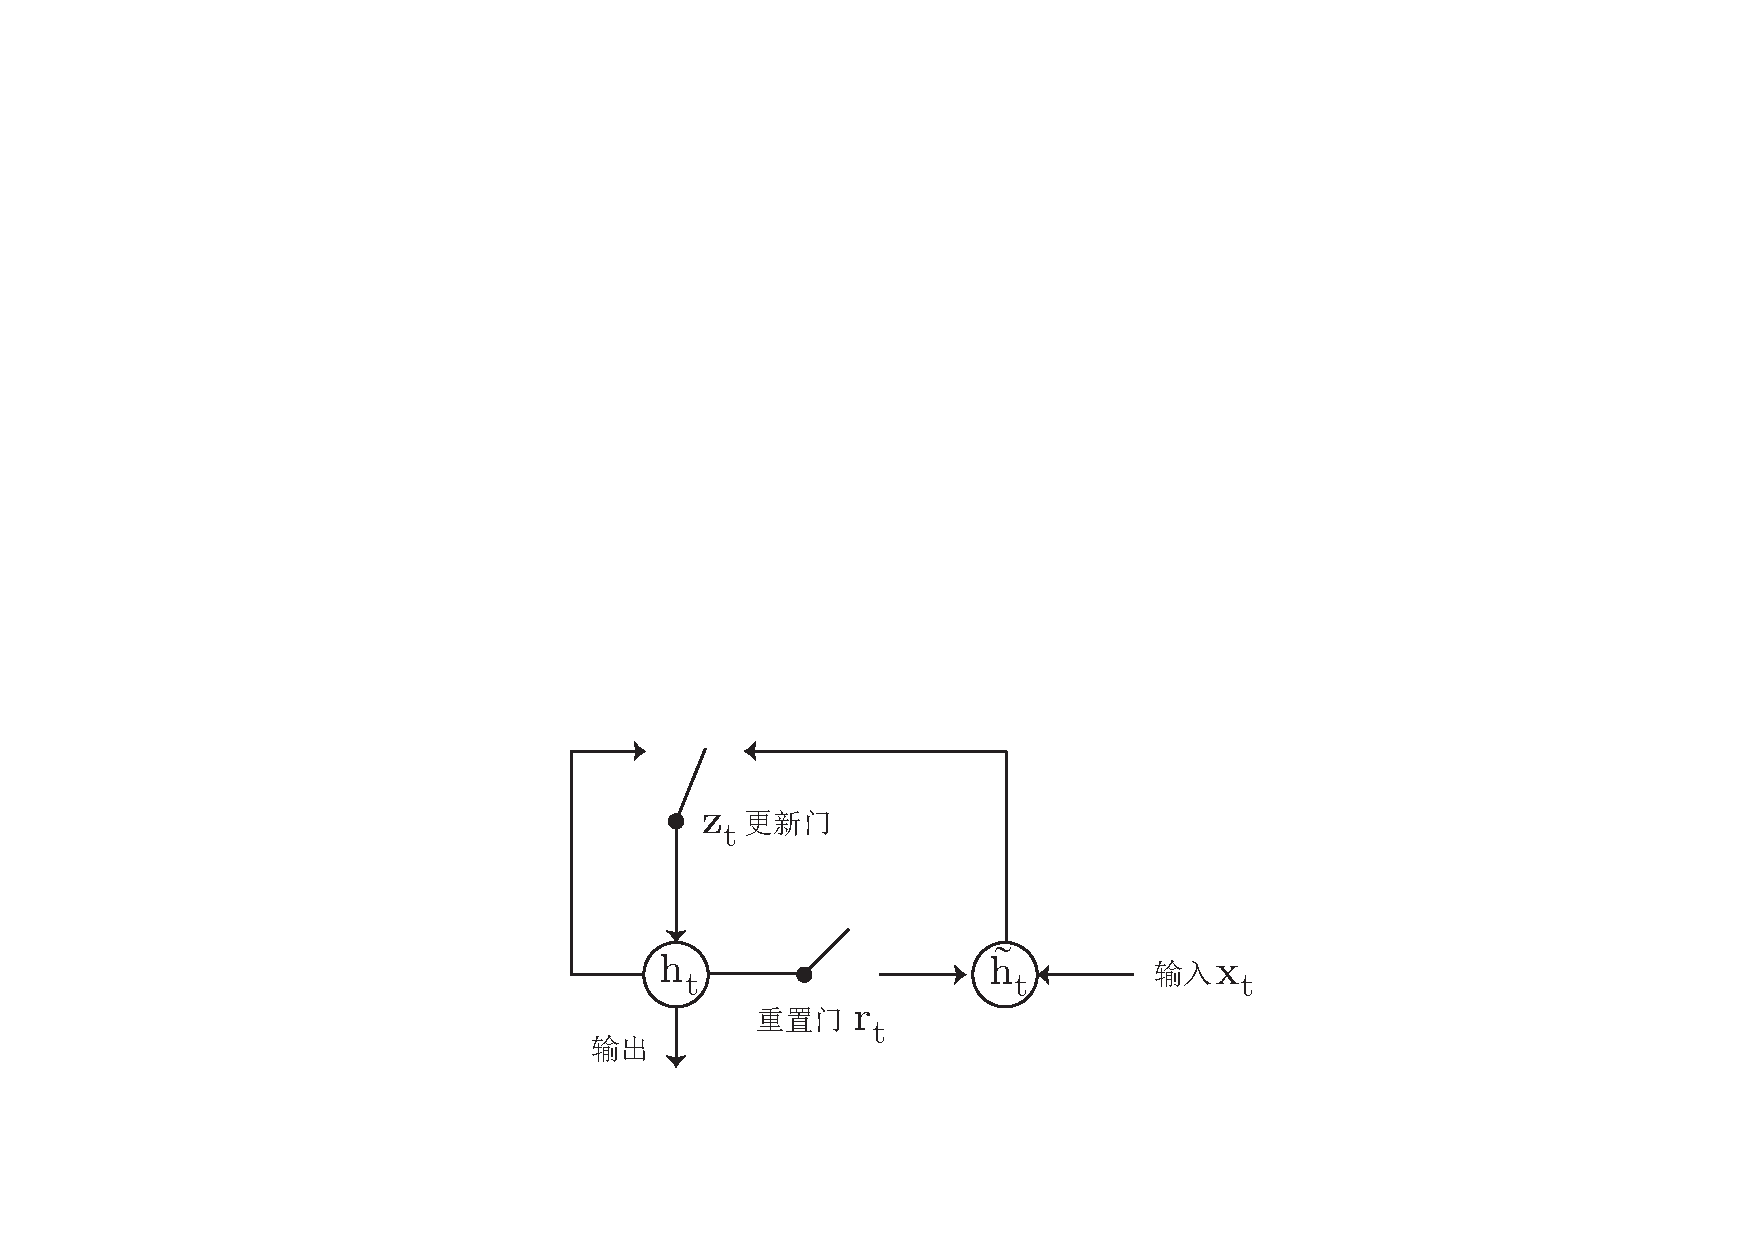
\includegraphics[width=0.6\linewidth]{./figures/gru.pdf}
  \caption{GRU模型示意图}\label{fig:gru}
\end{figure}

接下来我们介绍基于LSTM简化的模型,门限记忆单元(GRU)把 LSTM模型中的遗忘门$f_t$和输入门~$o_t$~用更新门$z_t$ 替代。同时,它把~Cell~的状态值和隐状态~$h_t$~进行了合并。 图~\ref{fig:gru}~是GRU更新~$h_t$~的过程\upcite{DBLP:journals/corr/Pezeshki15}, 主要包括:更新门~$z_t$、 重置门 $r_t$ 和节点内部更新值$\tilde h_t$和隐藏层输出值~$h_t$, 这里与~LSTM~的区别是GRU中没有输出门,其计算公式如下:
\begin{equation}\label{equ:gru}
\setlength{\abovedisplayskip}{10pt}
\setlength{\belowdisplayskip}{10pt}
\begin{split}
   z_t &= \sigma ( W^z x_t+ U^z h_{t-1}) \\
   r_t &= \sigma(W^r x_t  + U^r h_{t-1}  )\\
   \tilde h_t  &= \tanh (W^h x_t  + U^h(h_{t-1} \odot r_t) ) \\
   h_t &= (1-z_t)\odot \tilde h_t  + z_t \odot h_{t-1}
\end{split}
\end{equation}
如果重置门~$r_t=0$,那么计算~$h_t$~时将会丢弃之前的所有信息,即:$\tilde h_t=\tanh W^h x_t$; 若~$z_t=1$,模型直接把前一刻隐藏层输出~$h_{t-1}$~复制到当前时刻~$h_t=h_{t-1}$;如果~$r_t=1,z_t=0$,则~GRU~模型变成了一个传统的~RNN~模型,它只能处理短距离依赖问题。


\section{大词表问题}
softmax~函数通常用于多标签分类(Multi-class Classification)问题中的概率归一化(Probability Normalization)。考虑到~softmax~函数中包含除法操作,容易导致模型求解导数出现~NaN(Not-a-Number)现象,通常直接计算log-softmax函数。然而当分类的目标变多时,即对于语言模型的大词表问题中,softmax~函数会占用绝大部分计算时间,需要我们对这个计算瓶颈做更详细分析。这里我们首先给出~softmax,log-softmax~函数和相应的梯度(Gradient)的定义:
\begin{equation}\label{eq:softmax}
\setlength{\abovedisplayskip}{10pt}
\setlength{\belowdisplayskip}{10pt}
\begin{split}
p(w|h)=&\frac{\exp(h^\top v_{w})}{\sum_{w_j\in \mathcal{V}}{\exp(h^\top v_{w_j} )}} \\
\frac{\partial p(w_i|h)}{\partial v_{w_j}}=&p(w_j|h)(\delta_{ij}-p(w_i|h))h^\top\\
\end{split}
\end{equation}
\begin{equation}
\setlength{\abovedisplayskip}{10pt}
\setlength{\belowdisplayskip}{10pt}
\label{eq:log-softmax}
\begin{split}
\log p(w|h) &= \theta^w h-\log \sum_{u\in \mathcal{V}}{\exp(\theta^u h)}\\
\nabla_{\theta^u}{\log p(w|h)}&= (\delta_{uw}-p(w|h))h
\end{split}
\end{equation}
其中~$h$~指代的是隐藏层输出的向量(即上下文表示),$\theta^w$~表示单词~$w$~的目标单词向量~\upcite{duda2012pattern}。
公式中的克罗内克~$\delta$~函数~$\delta_{uv}$(Kronecker Function)定义为:如果~$u,v$~指的是相同的单词结果是~$1$,如果~$u,v$指的不是相同的单词则是~$0$。第一行计算公式指的是~softmax~函数,第二行计算公式指的是~softmax~函数的导数,第三行计算公式指代的是~log-softmax~函数,第四行计算公式指代的是~log-softmax~的导数。


如公式~(\ref{eq:softmax})~和~(\ref{eq:log-softmax})~所示,前向概率传播函数~$\log p(w|h)$(即第一行方程)和后向梯度优化函数${\partial p(w_i|h)}/{\partial v_{w_j}}$(即第二行的方程)都需要计算目标词汇表中的所有单词,因此在该部分上花费的时间会随着词表中包含的单词数量的增加而线性地增长~\upcite{DBLP:conf/acl/ChenGA16}。举例来说,假设词表中包含~$\mathcal{|V|}$~数量的单词来说,总的时间复杂度(Time Complexity)是~$\mathcal{O}(\mathcal{|H||V|})$,其中~$\mathcal{|H|}$~表示的是隐藏层输出的维度。代码实现过程中,softmax~函数被分解为:计算矩阵乘法(Multiply),计算求和函数(Summary),计算概率归一化的除法函数(Divide),第一步乘法操作占用了主要的计算时间。而且,目前的~GPGPU~设备的显存(Graphical Memory)是相当有限的,通常~Nvidia~公司提供的设备为~12GB~显存,目前最大的计算设备~Nvidia-K80~显存为24GB,然而这个设备造价相当昂贵\footnote{https://www.nvidia.com/zh-cn/data-center/tesla/}。因为我们不能任意增大显存大小,所以对词表大小有一个天然的上限。另一种缓解大词表存储问题的方法是进行多显卡训练,将大规模词表矩阵存储在单独的显存上。

我们需要区分~softmax~概率计算瓶颈是来自求和函数还是矩阵乘法函数。
softmax~算法的计算瓶颈不能归因于方程~\ref{eq:softmax}~中的循环函数~$\sum_ {u \in \mathcal {V}}$,尽管它随着词汇量的增长而线性增长,但是矩阵和张量的乘法计算的更消耗时间。所以相比于循环函数而言,主要的计算时间用于矩阵乘法计算。所以只有那些避免大矩阵乘法运算,即避免计算其他冗余字的概率才能达到最大的速度收益,而那些仍然涉及全局概率归一化的方法,并不能真正改善~softmax~占用的计算时间,那些优化求和函数的计算效率所获得的实际收益是微乎其微。


因此,在保证模型计算准确度不下降的情况下,我们期望能缓解概率归一化函数的计算瓶颈进而提高模型的训练速度。 目前能有效缓解大词表问题的算法主要分为以下三类: 单词拆分算法(Vocabulary Truncation)、采样估计模型(Sampling-based Approximation)和词表层次分解算法(Vocabulary Factorization)。下面将对三种不同思路的算法进行详述。



\subsection{单词拆分算法}
针对大词表问题,最直接、最简单的策略就是我们放弃使用大词表,转而保留较小的高频词来保证训练和测试的时候模型的内存(Memory Footprint)占用小和计算效率高。当我们只保留高频词,就会剩下很多其他不在词表中的单词被映射成~$\langle$unk$\rangle$。这相当于直接丢弃部分输入信息,可能使模型的训练变差。那么针对剩余的过多的词表外的单词(Out-Of-Vocabulary,OOV), Schwenk~等人提出可以使用传统的~N-gram~语言模型来估算其可能的概率分布~\upcite{DBLP:journals/csl/Schwenk07}。
这样做一方面保证神经网络模型可以在有限时间内训练完,同时保证模型的最后的测试结果不会很差。

然而我们需要注意到,当我们的词表继续减少并且我们选取的训练样本包含的不同的单词数量不断增加的时候,我们会发现训练样本中存在过多的~$\langle$unk~$\rangle$~字符,这直接导致转换后的句子变成了无法阅读者理解的句子,导致输入模型的信息噪声非常大,使得神经网络的模型训练非常困难,进而导致模型效果变得非常地差。所以这种方案只是一定程度上缓解了大词表问题,但是不失为一种简单且有效的尝试方案。

除了上述直接的建模方案外,目前采用的方案是将单词按照字符级别来划分。英文单词是由多个字符(Character)组成的,可以将一个单词按照字符统计规律划分成任意多个子词(Sub-word)。例如,Tucker~等人提出利用二元对编码(Byte Pair Encoding,BPE)将一个单词划分成前缀(Prefix)和后缀(Suffix)两部分~\upcite{DBLP:conf/icassp/Tucker0P94, DBLP:conf/acl/SennrichHB16a,Gage:1994:NAD:177910.177914},如图~\ref{fig:subword} 所示。从该图中我们可以看出,单词被划分成前缀和后缀两部分,其中$+$代表是单词的前缀,同时~$\langle /w \rangle$~是单词的后缀。
由于划分规则是从训练数据中学习到的,我们可以指定需要缩减的词表大小,所以该算法的动态适应性很强。
最初~Kucker~等人提出该算法目的是文本信息压缩(Zip软件),后来~Sennrichr~等人将该算法应用在目前主流的机器翻译模型中,获得很好的精度和性能收益~\upcite{DBLP:journals/corr/JozefowiczVSSW16}。
后续的提出的算法中,直接将单词拆分成字符序列(英文字符、数字和标点符号总共包含94个符号),模型训练得到的将不再是词向量而是字符向量(Character Embedding)。在测试的时候,我们将通过组合子词向量或者字符向量来获得这个单词的实际词向量。尽管如此,我们仍然需要看到它这样将单词解构成前缀和后缀的操作依然带来了一定的损失,因为句子的长度加倍对循环神经网络学习长距离关系能力提出了更高的挑战~\upcite{DBLP:conf/aaai/KimJSR16}。

\subsection{采样估计模型}
第二种策略也是通过减少单词数量从而减少计算量。与上面直接将单词拆分成子词不同的是:这种算法是在训练的时候,通过采样算法选择少量单词,用来估计softmax~函数的可能的概率分布。因为实际只有一个单词是需要预测的,其他的单词都是可以认为是噪声单词。

目前流行的采样算法(Sampling Algorithm)主要是针对公式~(\ref{eq:softmax})~中对所有单词概率规约那一项进行概率估计,可以分类为:重要性采样(Importance Sampling)~\upcite{DBLP:journals/tnn/BengioS08},噪声差分估计(Noise Contrastive Estimation,NCE)~\upcite{DBLP:conf/icml/MnihT12}和~Blackout~采样算法~\upcite{DBLP:journals/iclr/JiVSAD15}。第一种算法在~Bengio~等人的论文实验中被证明模型无法收敛~\upcite{DBLP:journals/tnn/BengioS08},因此目前主流模型都使用后面的两种采样算法,所以我们仅对后面两种方法进行概述。

对于~NCE~噪声差分估计算法来说,模型的学习目标是区分将正确的单词~$w_0$~与随机生成的单词~$\{w_1\cdots w_k\}$。
其中~$w_0$~指代的是训练样本中真正的下一个单词,$\{w_1\cdots w_k\}$~是采用先验分布~$q(w)$~产生的随机噪声单词。实际实验中,我们常用的采样的概率分布模型~$q(w)$~是单词词频分布(Word Frequency Distribution)。正例归一化后的概率~$\tilde{p}(y=1|h)$~和所有负例联合概率~$\tilde{p}(y=0|h)$~的公式可以写成如下形式:
\begin{equation}\label{equ:nce}
\setlength{\abovedisplayskip}{10pt}
\setlength{\belowdisplayskip}{10pt}
\begin{split}
  \tilde{p}(y=1|h)=&\frac{\exp( \theta^w_0 h)}{ \exp( \theta^w_0 h)+k *q(w_0)}\\
  \tilde{p}(y=0|h)=&\prod_{i=1}^{k}\frac{k *q(w_i)}{\exp( \theta^w_i h)+k *q(w_i)}\\
\end{split}
\end{equation}
噪声概率~$\tilde{p}(y=0|h)$~仅对~$k$~个噪声样本做加和运算而不是对整个词表进行运算的,因此该算法的计算复杂度就是~$\mathcal{O}(k+1)$,所以该算法与简单的~softmax~算法计算复杂度的比值是~$\mathcal{O}(\mathcal{|V|}/(k+1))$。

除了上面这种最经典的算法之外,后续又衍生出了其他的采样算法。
最近才提出的~Blackout~采样算法针对噪声概率归一化的时候~$\{w_1\cdots w_k\}$~与当前上下文的关系,对上述的~NCE~算法进行了进一步优化和修正~\upcite{DBLP:journals/iclr/JiVSAD15},同时也对模型引入了更多的计算量,计算公式如下所示:
\begin{equation}
\setlength{\abovedisplayskip}{10pt}
\setlength{\belowdisplayskip}{10pt}
\begin{split}
&\ell=-\log(p(w_0|h)) - \sum_{w_i \sim q(w)} \log(1 - p(w_i))\\
&p(w_i) = \frac{\exp(\theta^w_i h)}{\sum_{w_i \sim q(w)} \exp(\theta^w_i h)}
\end{split}
\end{equation}

总的来说,这些采样近似算法可以显著加快训练速度,但仍然需要利用单词分布$q(w)$~\upcite{DBLP:conf/naacl/ZophVMK16}来采样大量的噪音单词,在采样单词足够多的情况占用的时间仍然很可观,需要进一步的手段去优化。
另一方面,在推理测试时无法预知单词的概率分布更无法得知正确的单词是什么,只能调用~softmax~函数计算单词概率分布,意味着该算法无法应用在测试推理阶段~\upcite{DBLP:journals/jmlr/GutmannH12}。
同时,由于在做采样估计时引入了采样函数~$q(w)$,模型将会花费额外时间在采样计算上,因此我们需要寻找一个性能优异的离散采样函数(Discrete Sampling Function)或者是带权重的随机数生成器(Weight Random Number Generator)。


\subsection{词表层次分解}
介绍完单词拆分、采样估计算法后,第三种层次分解方法(Factorization)可以有效降低训练和推理过程中计算概率分布所占用的内存,因为它只计算局部概率(Local Probability)并且选择每一层的分数最高的候选路径而不是保存全局计算结果。
目前主要的分解策略可以分为:基于类别的多元分类模型(Class-based Hierarchical Softmax,cHSM)和基于二叉树的二元分类模型(Tree-based Hierarchical Softmax,tHSM)。接下来我们介绍这两种算法的计算过程。

首先我们考虑基于类别的分解策略。假设文本所对应的词表被划分成各个类簇,每个单词只属于一个类(Class或者Group)。在此假设之上,单词在在语料中的概率分布可以转化为:先计算类别的概率分布,然后乘以在所属类上该词的概率分布~\upcite{王龙2015基于循环神经网络的汉语语言模型并行优化算法}~,于是可将公式~(\ref{eq:softmax})~转化为如下形式:
\begin{equation}
\setlength{\abovedisplayskip}{10pt}
\setlength{\belowdisplayskip}{10pt}
\begin{split}
&p(w|h)=p^c(\mathcal{C}(w)|h)\cdot p^w(w|\mathcal{C}(w),h) ,\\
 & w\in \mathcal{C}(w),\mathcal{V}=\bigcup _{i = 1}^\mathcal{C}{c_i}, \quad  c_i \bigcap c_j=\phi, \text{若}\quad i\ne j, \\
\end{split}
\end{equation}
其中第一项概率~$p^c(\mathcal{C}(w)|h)$~表示每个类别的概率,第二项概率~$p^w(w|\mathcal{C}(w),h)$~表示在类别$\mathcal{C}(w)$中所有单词的局部概率。

该模型计算一个词的概率分布所需要的计算复杂度正比于: $\mathcal{O =|H||C|}$。 在该计算公式中,$\mathcal{C}$~表示的是该语料中所有词的分类数目,我们可以按照不同策略划分词表,最简单的一种策略就是根据语料中词的词频进行均匀划分。 当$C$ 取$1$ 或取词表大小~$|V|$~时,此结构等同于标准的~softmax~结构,此时词表还是原来的结构,并没有任何优化效果。因此,对于绝大多数情况,我们取$\mathcal{C} \ll \mathcal{V}$并且 $|\mathcal{C}|\ll 1$,这样的结构才能保证有效降低~softmax~的计算复杂度。图~\ref{fig:case_hsm}~展示了类别划分和分步概率计算的过程。如图图~\ref{fig:case_hsm}~所示,词表 [duck,cat,mop,broom,the,am] 被划分成三个类别:$c_1\to$[duck,cat],$c_2\to$[mop,broom]并且$c_3\to$[the,am]。
\begin{figure}[!t]
  \centering
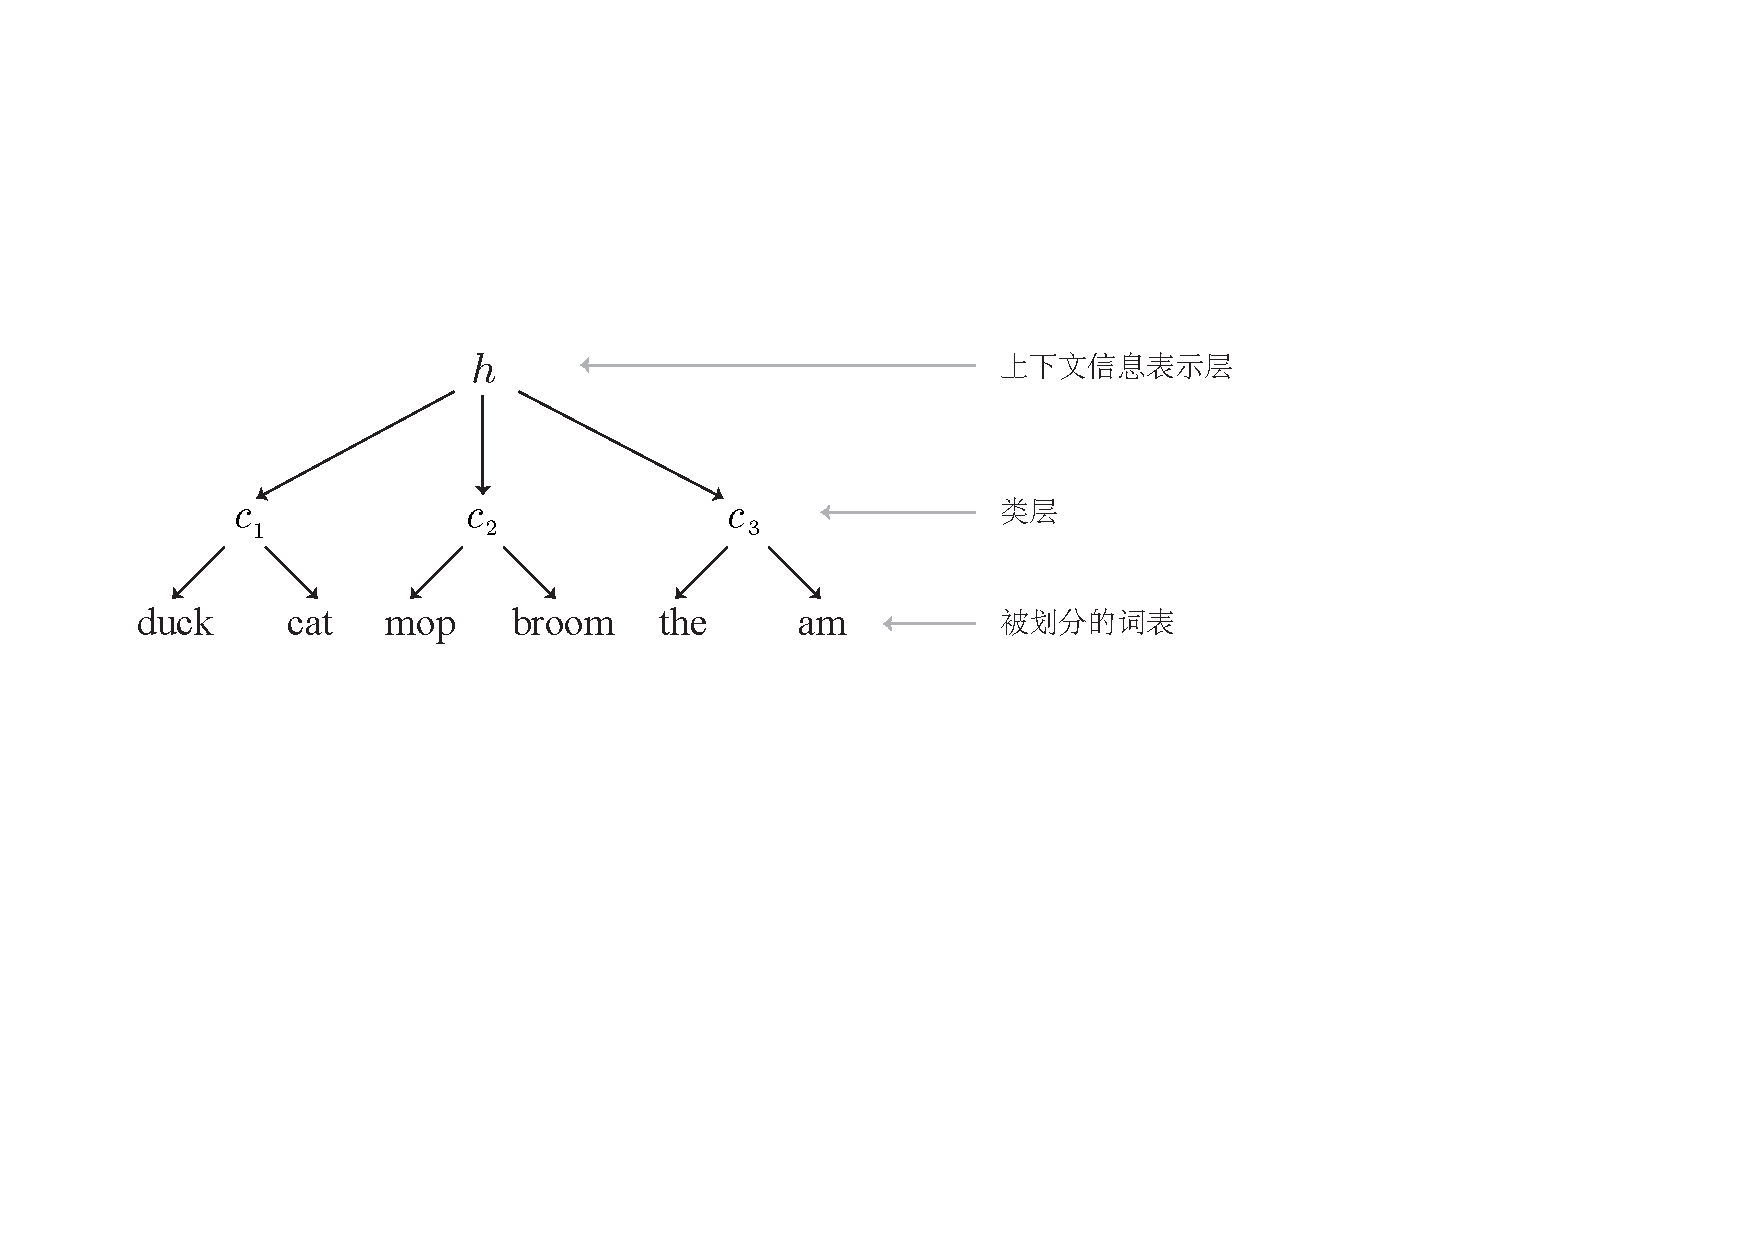
\includegraphics[width=.9\linewidth]{./figures/case_chsm.pdf}
\caption{cHSM算法可视化模型}\label{fig:case_hsm}
\end{figure}

接下来分析基于类别的分层模型计算速度提升效果。假设每个类包含~$\sqrt{\mathcal{|V|}}$ 单词,表示词汇被划分为相同大小的组,这样的话级联概率(Cascaded Probability)只涉及~$2\sqrt{\mathcal{|V|}}$~单词 softmax计算,所以最优时间复杂度可以减少到~$\mathcal{O}(\mathcal{|H|}\sqrt{\mathcal{|V|}})$~\upcite{DBLP:conf/icassp/Goodman01}。虽然在更常见的情况下,词表划分算法会产生不同大小的分组,这需要其他结构来支撑这种非均匀划分操作,尚未被完全探索和实验分析。此外,我们还可以通过调整不同的类数目和词表划分算法来调整模型的精度和效率。

另一方面,我们再介绍基于二叉树分解词表的建模策略。tHSM~方法将单步骤分类过程分解为多步骤二元分类步骤。正因为如此,词汇组织为二叉树,其中单词分布在二叉树的叶子节点上,二叉树的所有的中间节点的都是内部参数。在该二叉树是平衡树(Balanced Binary Tree)的结构情况下,每个词将会被赋予相等长度的0,1路径,最优时间复杂度可以减少到$\mathcal{O(|H|\log \mathcal{|V|})}$。图~\ref{fig:case_thsm} 展示了一颗平衡二叉树词表分解和访问路径的示例。关于如何构建这颗二叉树,最早的工作中单词在二叉树上的分布可以由WordNet与领域专家~\upcite{DBLP:conf/aistats/MorinB05}或由单词~Uni-gram~分布~\upcite{DBLP:conf/nips/MikolovSCCD13}推导的霍夫曼编码构建。然而,在大规模文本应用中,专家知识的构建是相当昂贵的。所以,一般不会采用这样的方案来构建单词的二叉树分布,霍夫曼编码方案只考虑单词词频信息,而单词的句法或语义信息尚未被利用和得到彻底的分析讨论。

\begin{figure}[!t]
  \centering
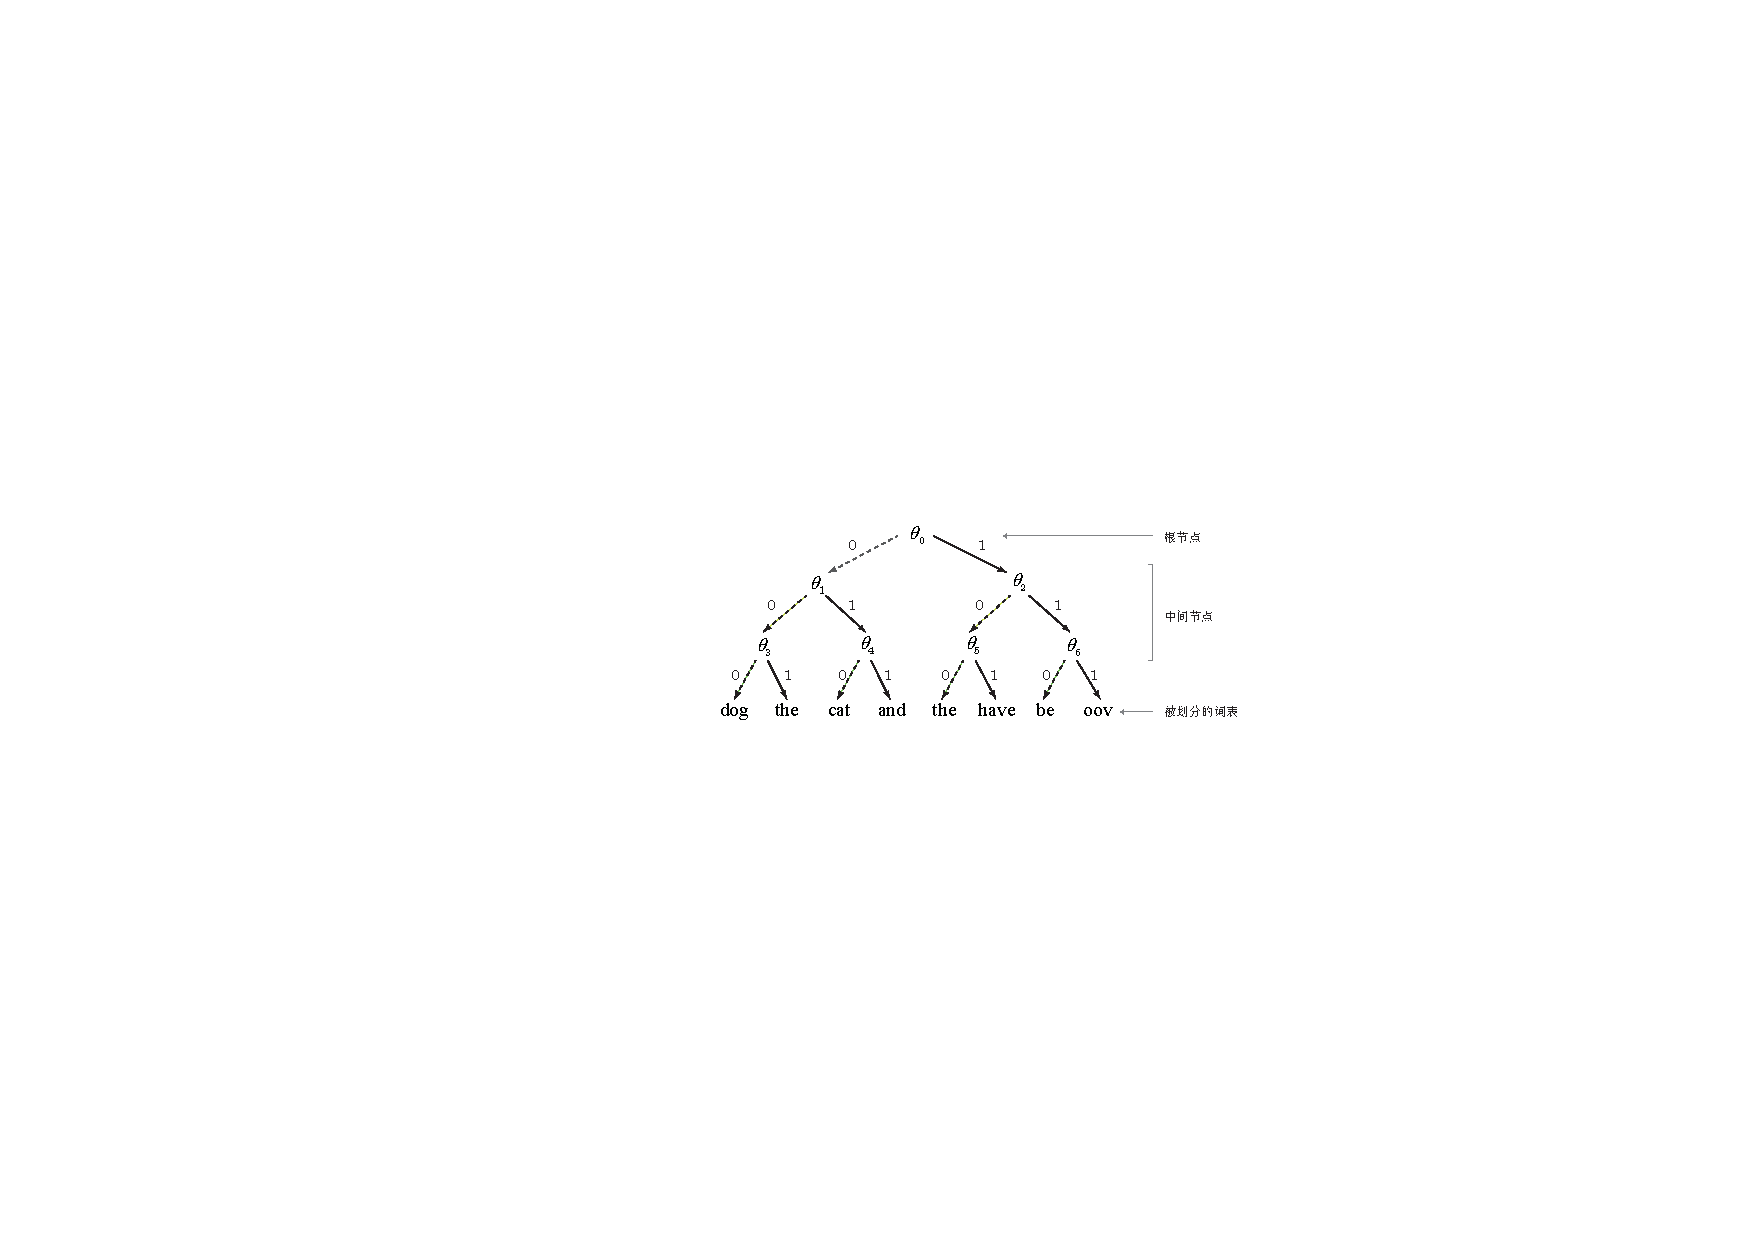
\includegraphics[width=.85\linewidth]{./figures/thsm-example.pdf}
\caption{tHSM算法可视化模型}\label{fig:case_thsm}
\end{figure}

\section{离散采样算法}
\begin{figure}[!b]
  \centering
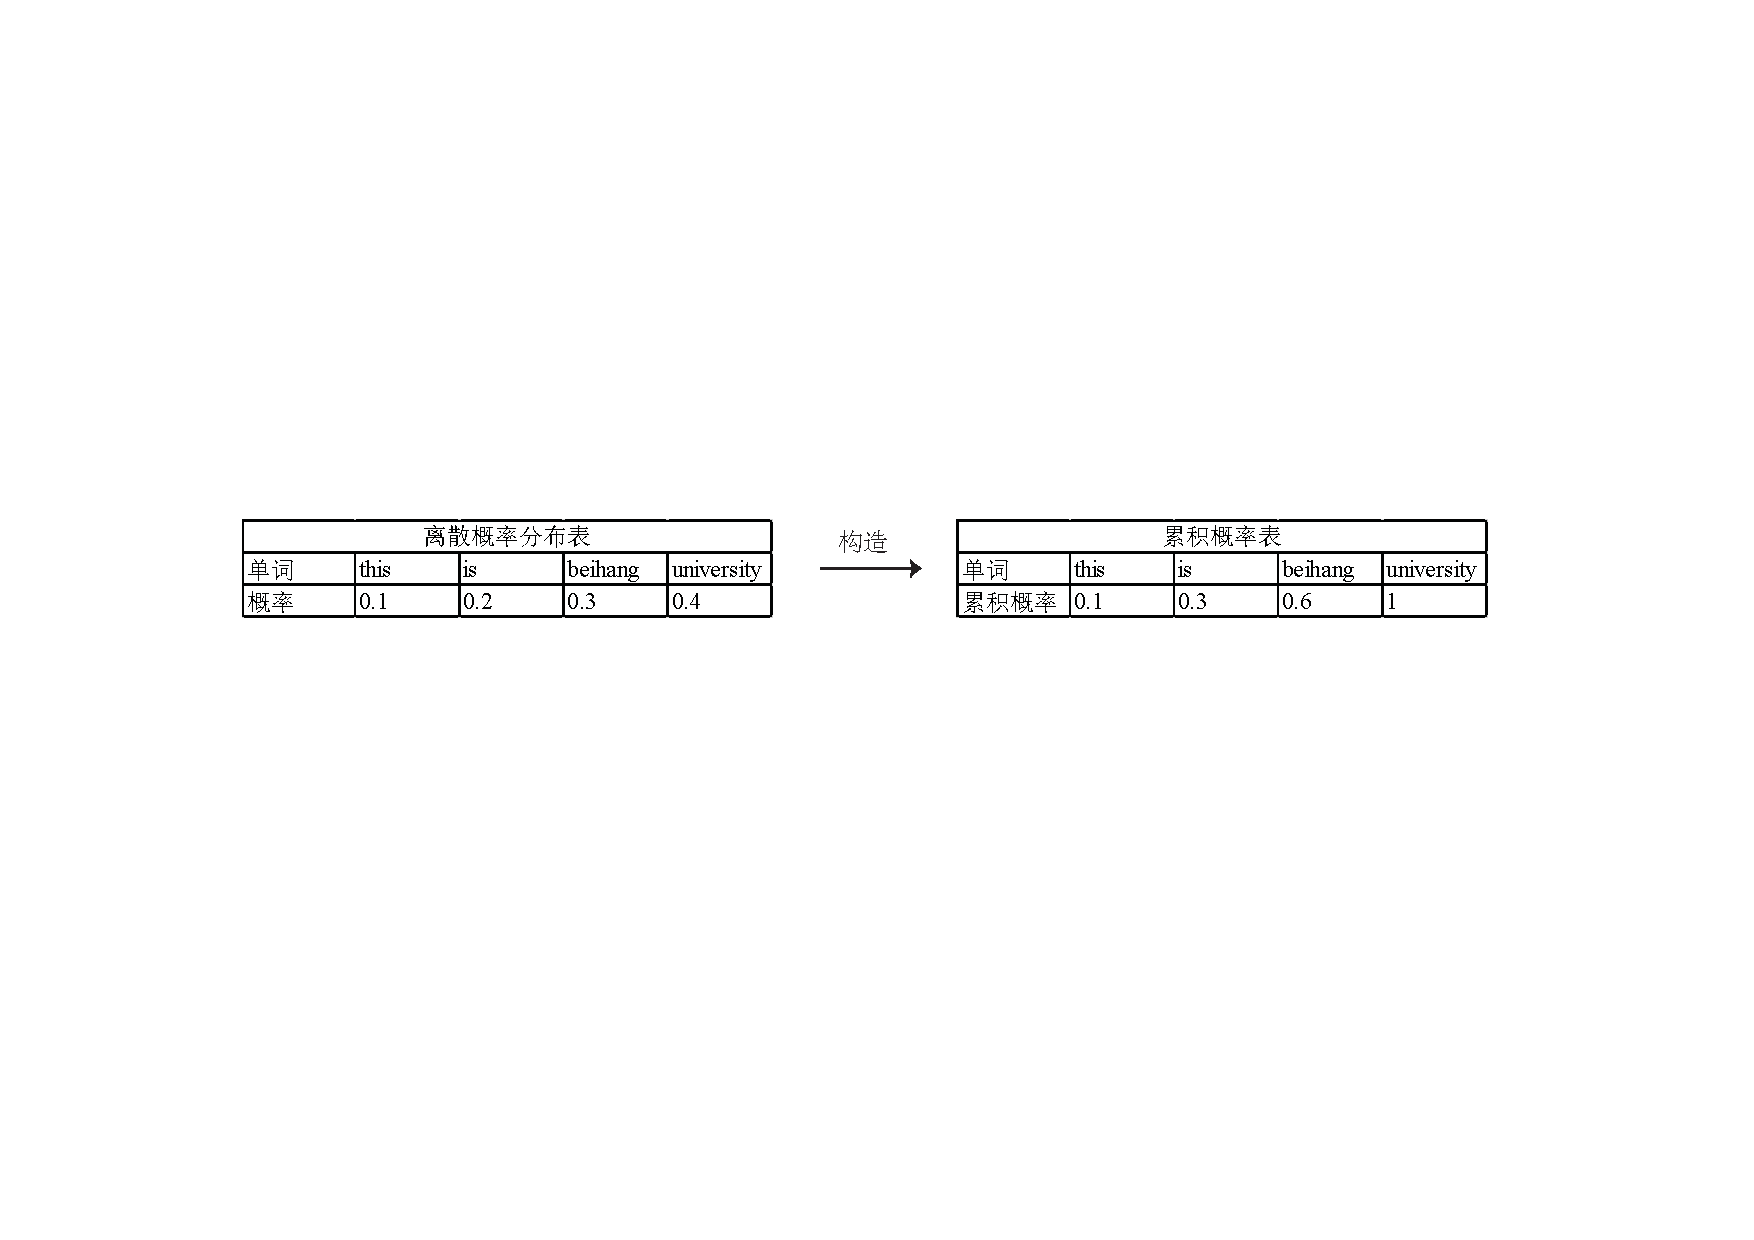
\includegraphics[width=1\linewidth]{./figures/cdfreverse.pdf}
\caption{由离散概率分布构造累积概率分布}\label{fig:cdf_reverse}
\end{figure}

前文提到在使用基于采样估计模型时,不可避免地需要使用到离散采样函数,我们在这一个部分来讨论构建高效离散采样函数的策略。首先给出离散采样问题的定义:设一共有~$|\mathcal{V}|$~个单词,第~$i$个~单词~$w_i$~出现的概率是~$p(w_i)$, 如何高效地产生这样的随机变量序列~$w_1,w_2,\cdots$?该问题被称之为模拟离散取样(Simulated Discrete Sampling),其含义指的是根据有限类别的非均匀概率分布,来模拟有放回的采样,从而生成需要的采样序列。因为计算机只能快速产生伪随机数(Psudo Random Number Generator),即对均匀分布(Uniform Distribution)做采样,其他的复杂采样函数均建立在均匀分布的变换之上。所以该问题的关键就是如何将均匀分布变换到实际变量的分布,生成指定概率分布的随机单词序列。

如图~\ref{fig:cdf_reverse}~所示,首先将离散概率分布转换成累积分布函数表(Cumulative Distribution Function,CDF)。我们可以使用Matlab代码,很容易地完成这个计算过程。如图~\ref{fig:sample}~所示,所展示的代码使用了线性搜索算法(Linear Search)。该算法很简单,最容易实现。但是注意到该算法初始化的时间复杂度是~$\mathcal{O(\mathcal{V})}$~。计算每个样本时的时间复杂度也是~$\mathcal{O(V)}$。
\begin{figure}[!t]
  \centering
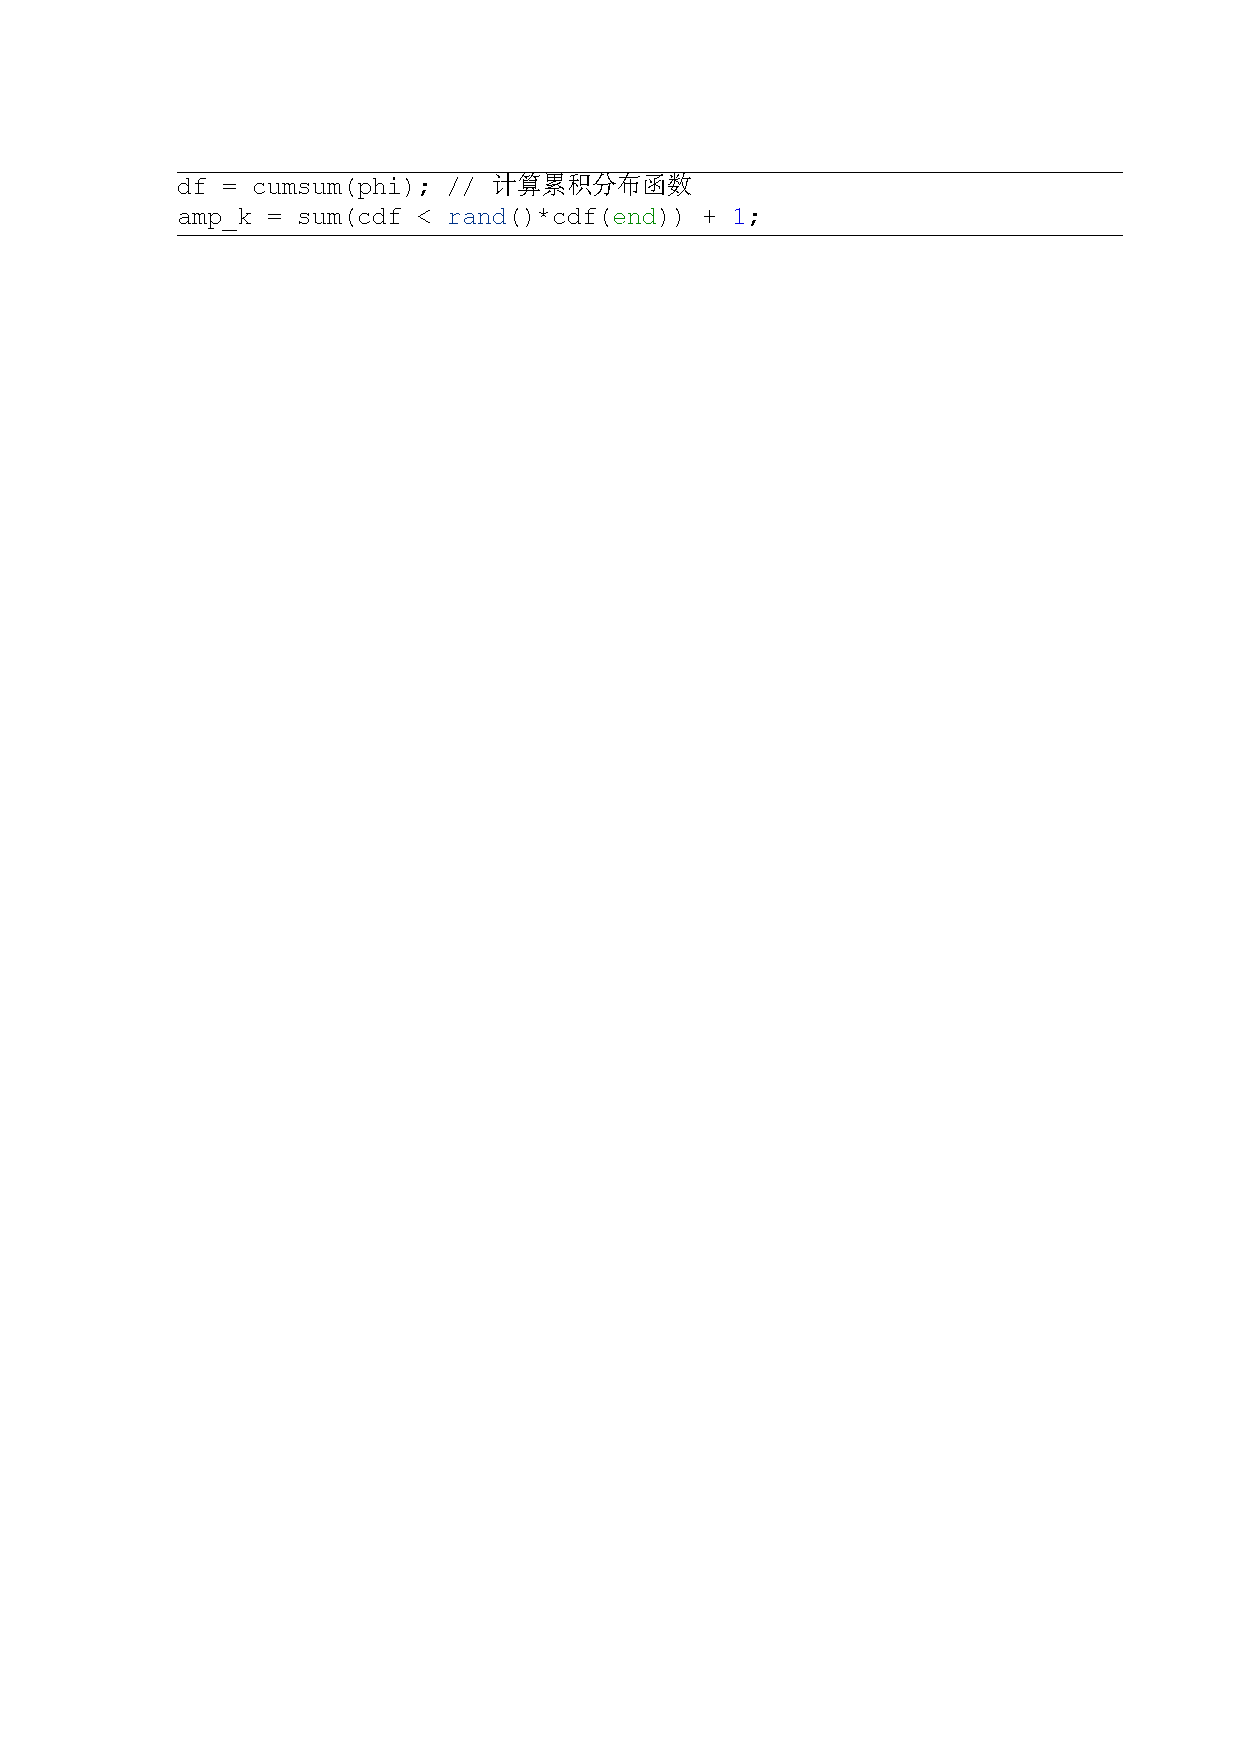
\includegraphics[width=1\linewidth]{./figures/cdf.pdf}
\caption{Matlab实现的离散采样函数}\label{fig:sample}
\end{figure}


考虑到该累积分布是从小到大顺序组织的,可以使用数据结构中的查找算法更快地找到结果。我们可以采用从左至右的方式线性搜索随机数所在的区间,其时间复杂度是$\mathcal{O}(\mathcal{V})$;也可以使用更高效的二叉搜索(Binary Search)快速计算随机数所在的区间,对应的时间复杂度是$\mathcal{O}(\log \mathcal{V})$。



在~$\mathcal{V}$~很小的情况下,使用线性查找算法或者二分搜寻算法也足够得快;当~$\mathcal{V}$足够的大,即所谓的大词表问题的时候,我们可以采用别名方法(Alias Method)\upcite{DBLP:reference/stat/LEcuyer11}、近似方法等~\upcite{DBLP:journals/cgf/ClineRW09}。本实验采用别名算法,该算法利用两次随机采样来生成采样序列,具有恒定的~$O(1)$采样时间复杂度。该算法的精髓在于构造别名表(Alias Table),需要~$O(\log |\mathcal{V}|)$~构造时间复杂度~\upcite{10.2307/2683739,DBLP:conf/emnlp/VaswaniZFC13},具体构造方法可以参考\footnote{https://hips.seas.harvard.edu/blog/2013/03/03/the-alias-method-efficient-sampling-with-many-discrete-outcomes/}。

\begin{figure}[!t]
  \centering
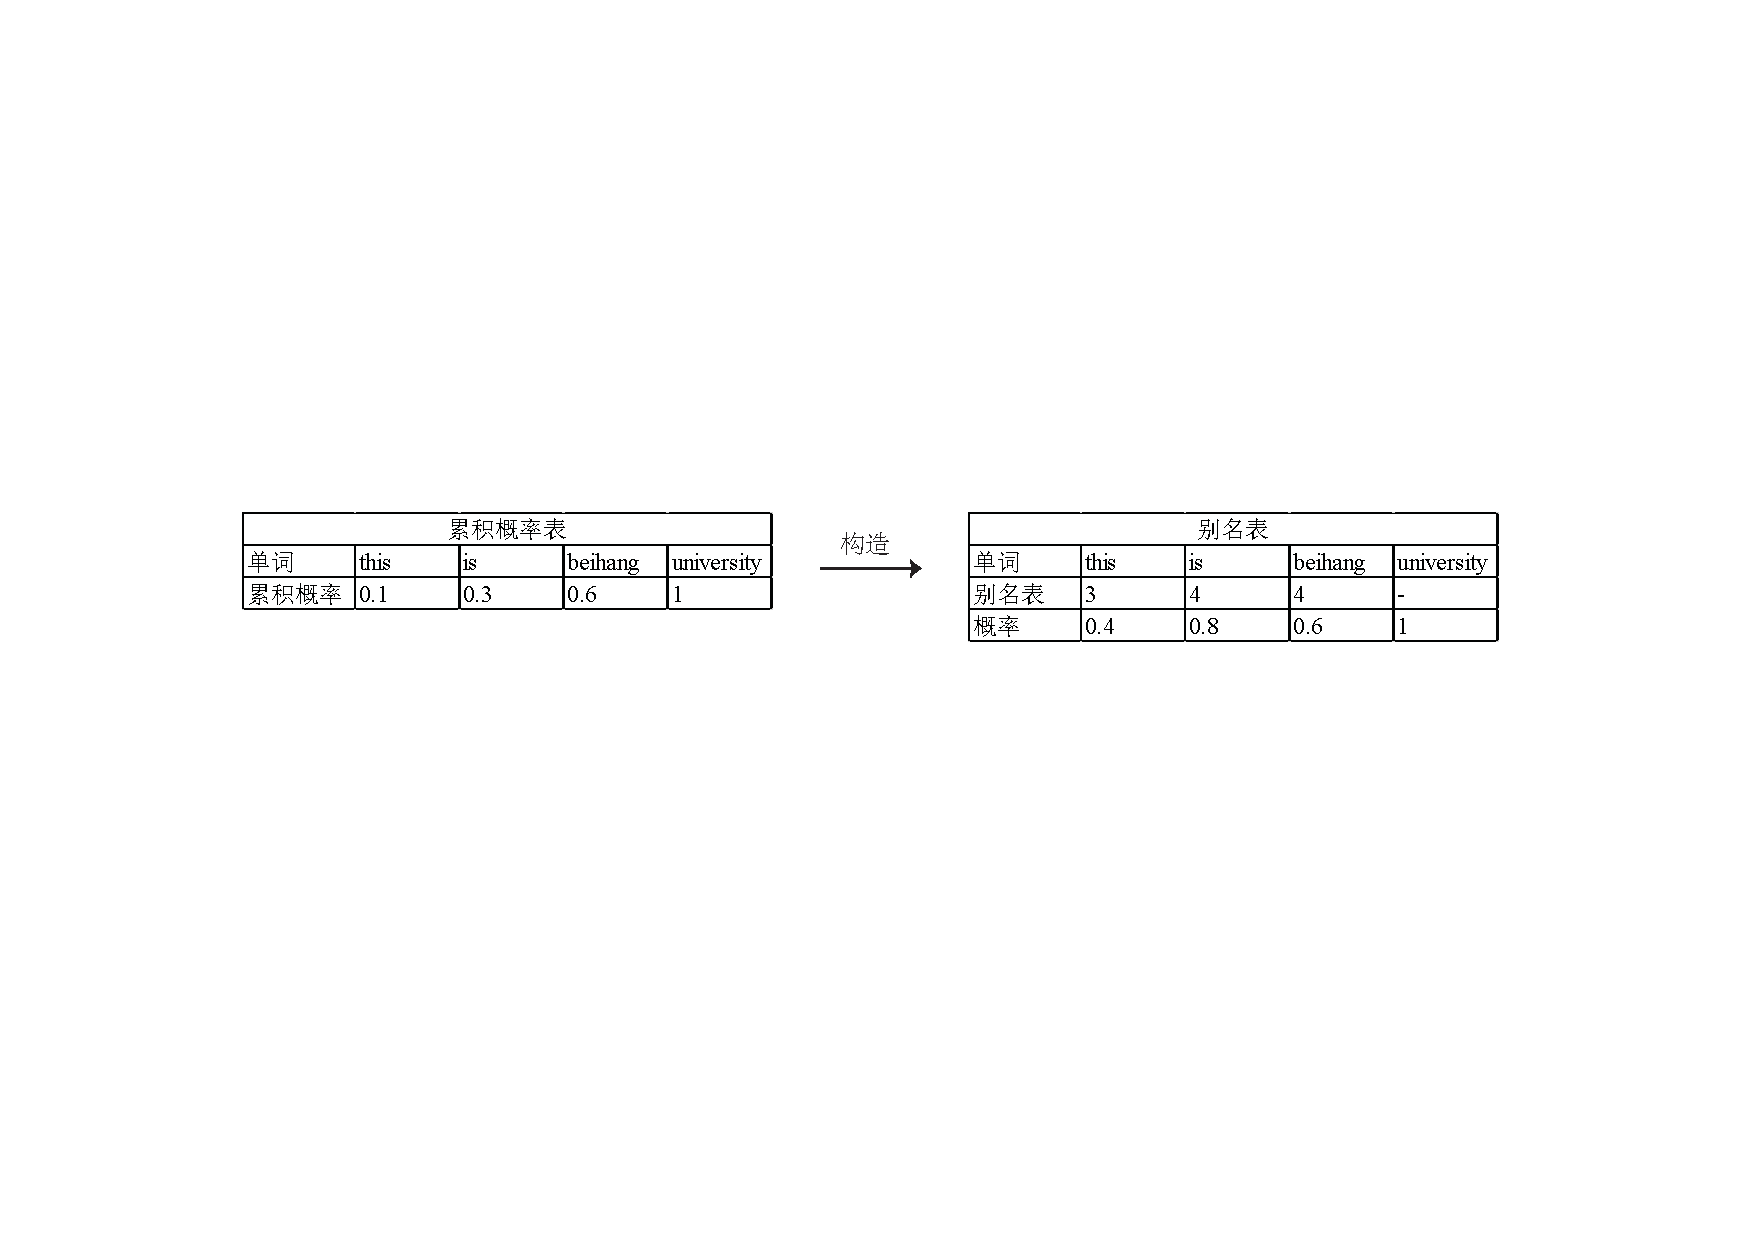
\includegraphics[width=1\linewidth]{./figures/alias.pdf}
\caption{由离散概率分布构造别名表}\label{fig:alias}
\end{figure}


\section{本章小结}
本章对国内外学者在语言建模任务上的相关工作进行了概述。首先介绍了语言模型的建模策略和对应的实际应用场景。其次详细讨论了循环神经网络的语言模型的建模方式,并讨论了其结构的优缺点。同时为了解决使用循环网络所带来的梯度爆炸问题,我们进而引入了长距离短期神经网络和门限记忆节点两种基于门限机制的循环网络;另一方面,我们还考虑了语言模型大规模应用所带来的大词表问题,并作了详细分析原因。
同时,还讨论了历史上所提出的解决方案,主要涉及三种思路:缩减词表大小,用采样算法近似估计和模型层次分解,我们对各种模型的结构做了概述,并分析了各种算法的优劣。最后分析了实验中需要用到的高效采样函数的构造算法。

%\RestyleAlgo{boxed}
\chapter{树状层次概率计算模型}
在本章中,我们考虑将预测端词表概率进行分步求解,来解决语言模型中遇到的大词表问题。我们将这个预测端的词表用二叉树的分层的形式表示,通过多次的逻辑分类算法判断二叉树的访问路径从而避免了对所有单词做归一化运算。为了使单词基于二叉树的路径的编码适配基于树的分层概率计算,我们首先提出了一个在二叉树分层结构上对单词进行极性编码的方案。与此同时,因为考虑到GPGPU设备上允许算法能并行计算,传统的基于CPU设备只能线性计算,这为我们算法的效率进一步提高提供了可能。为了保证算法的并行计算的高吞吐量,我们进而推导出二叉树概率模型的紧凑的代价函数以及其模型参数的梯度计算公式,使得该分层模型在GPGPU设备上的能并行地计算模型的每一层内部概率函数,而不是从根节点到叶子节点线性计地算模型内部各层的概率函数,避免浪费GPU设备的高并行性能的特性。

同时,我们需要注意到,由于所有单词都分布在这个二叉树的叶子节点上,单词的内部节点对于目前的模型无法包含单词只能作为单词的路径参数,所以需要我们在模型训练之前给一个初始化定义。然而不同算法所生成的基于二叉树上的单词分布,可能生成一颗平衡二叉树,也可能生成一颗霍夫曼二叉树,又或者是高度偏斜的二叉树,不同的树分布对其最终任务性能有很大的影响,所以应该在训练阶段之前就给出一个较为合理的单词分布。在本实验中,我们并不打算考虑那些在模型训练过程中动态交换二叉子树的算法进而调整和改变了单词在二叉子树上的分布结构, 而是采用了几种分层聚类策略,利用单词或者文本的统计信息,句法结构和语义知识和已有的层级聚类算法来初始化单词的二叉树分布结构,以达到一个稳定和可以预期的模型性能。另外,我们不考虑单词的一词多义的现象,即一个单词不会出现在两条不同的路径上,不同的的二叉树访问路径所对应的单词一定不相同。

另外,在语言模型的测试推理过程中,主要的两个任务可以分解为:1)给句子打分(Sentence Scoring)。输出给定单词序列的概率值;2)给定上下文,对所有的单词进行排序(Word Ranking)。在给定的上下文中选择获取得分最高的一个或多个候选单词。不同于传统的softmax算法情况,得到最好的候选者单词是天然可行的并且能直接被计算出来,层次推理模型不能直接应用 softmax 方法来实现。尽管我们可以计算出所有单词的概率,然后再依照softmax算法的情况类推,这样的计算方式是十分冗余的,直接将层次模型的计算优点给忽略了。因此,我们需要讨论并研究基于二叉树的搜索策略,以满足上述两种不同的推理情形。
\section{基于二叉树的单词极性编码}
首先,我们需要知道所有的单词分布在二叉树的叶节点上,因此我们可以通过访问从根到叶节点的所有内部节点来定位每个特定的词,所以不同的访问路径代表不同的单词。举例来说,单词~$w$~的路径表示所有内部节点~$\theta^w_i$~和它访问的边~$d^w_i$。

为了方便理解,首先直观上说明一下传统softmax和树状层次概率模型的差异点。可以认为传统的softmax将单词均匀放置在一个特征空间(Feature Space)里面。基于二叉树的算法则是首先将这个所有单词所在的特征空间划分成两个子空间(Subspace),这里没有规定空间划分必须均匀(Equal Partition),所以这两个子空间不一定相同。接下来,对每一个子空间,接着划分成两个更小的子空间,直到每个子空间里面包含的单词有且仅有一个为止。在模型计算概率的时候,更多的时候是计算特征划分到这个子空间的概率。
因此每次都需要计算二叉树访问路径的概率,这个概率值就是将模拟特征划分到这个子空间的可能性。
通过这个路径概率的求和我们可以避免对所有单词的概率计算,因为每次都做逻辑分类算法(Logistic Classification),只要计算一个分支的概率,由于两个分支的概率值之和一定等于1,另一个分支的概率可以直接推导出来,从而不需要再计算一遍了。


接下来,来说明传统二叉树编码和我们提出的编码方案之间的差异点。不同于传统的基于二叉树的单词的~$0,1$~编码方案,在模型中需要引入单词的极性编码方案(Polarity Encoding Scheme),即单词的路径是由$-1,+1$组成。其含义同原来的01编码方案类似,但他能帮助推导出更加简洁有效的模型代价函数。在上一章中,图~\ref{fig:case_thsm}~给展示了一个路径编码的例子。

\begin{table}[!t]
  \centering
  \caption{树状层次概率计算模型的符号助记表\label{tab:note}}
\begin{tabular}{llc}
  \toprule
   符号&含义&取值范围\\ \midrule
$l^w$ &单词$w$ 所对应的叶子节点和中间节点的路径&Int32 \\
$d_j$&表示路径$l^w$中第$j$个节点对应的编码(根节点对应编码$0$)&$ \{-1,+1\}$\\
$ d^w=[d_0^w,d_1^w,\cdots,d_{l^w-1}^w] $& 单词 $w$ 的极性编码,他由 $l^w-1$位编码构成,&$\{-1,+1\}^{l_w}$\\
$\theta_{j}^w\in\mathbb{R}^m$ &表示路径$l^w$中第 $j$ 个非叶子节点对应的向量& Float32\\
$ \theta^w=[\theta_1^w,\theta_2^w,\theta_3^w, \cdots,\theta_{l^w}^w]$&表示路径$l^w$所对应的参数矩阵&Float32 \\
$\Gamma$ &路径查找表,给定路径序列,可以获得对应的单词& ---\\
  \bottomrule
\end{tabular}
\end{table}

由于实际层次聚类算法(Hierarchical Agglomerative Clustering)产生的二叉树分布通常是不平衡的,所以不同单词的路径长度不一致,然而基于python语言的Numpy和Theano库目前都不支持动态长度的设置(Dynamic Type),所以需要介绍一下实际实现过程中用到的辅助计算矩阵,其结果和使用C++等动态语言所计算输出的结果是一致的,仅仅是因为实现语言框架的限制,导致引入这一操作。
需要注意到,对于平衡二叉树,所有单词的访问路径长度是一样的,所以不需要使用掩码矩阵。
对于非平衡二叉树,由于单词的访问路径长度都不是很相似,因此我们可以使用掩码矩阵来进行计算,在这里掩码矩阵标记为$\mathtt{bitmask}$。
当使用掩码矩阵时,相当于将非平衡二叉树填补形成一颗完全二叉树,如图~\ref{fig:case_thsm_mask}~所示。但是那些填补单词的子树都代表该单词,即:存在多条路径指代同一个单词,而在实际求解实验过程中,需要保证一条路径只对应一个单词,因为多余的计算路径会被掩码覆盖掉,无法反映在实际模型的代价函数里面。


接下来详细说明模型的编码方式和所涉及的参数,如表~\ref{tab:note}~所示。其中,$\theta_i^w $表示到达叶子单词节点$w$的路径上第~$i^{th}$~层上的非叶节点,并且$\theta_i ^ w$是一个 $m$维度的向量,即:$\theta_i^w \in\mathbb{R}^m $ 其中$ i \in [0, l^w-1] $。同样的,$ d_i^w $表示连接第$(i-1)^{th}$层和第$i^{th}$层节点的边。对于每个非叶子节点来说,向下移动到左边的分支标记为$ -1 $,选择右边的分支标记为$ + 1 $。因此:$i\in[0,l^w-1]$, $d_i^w\in \{-1,+1\}$。 除此之外, $l^w$~表示从根节点到叶子单词节点的路径长度。如果该二叉树是平衡树,即单词都均匀分布在同一层叶子节点上,那么二叉树的深度(Tree Depth)是$l^w\approx \log \mathcal{|V|}$ 。通过这个编码方案,可以使用极性路径来定位每个单词,即:将单词索引(Indexing)或稀疏向量表示(Sparse Representation)改变为单词极性编码元组$(d^w,\theta^w)$。



在实际运行环境中,需要通过维护一个路径查找表$\Gamma$(Path Looking-up Table),用来记住每个单词$ w $从根到叶的所有访问内部节点的索引。这样,就可以从$ \Gamma(w)$中选择对应行的所有节点,从参数矩阵${\Theta} $中检索$ \theta ^ w $。其中${\Theta} $的第一维的维度是:
\begin{equation}\label{equ:sums}
\setlength{\abovedisplayskip}{10pt}
\setlength{\belowdisplayskip}{10pt}
\sum_{i=0}^{\log \mathcal{|V|}}{2^i} =2^0+2^1+\cdots+2^{\log \mathcal{|V|}}= \mathcal{|V|} -1.
\end{equation}
因此,p-tHSM模型没有增加模型额外参数,除了预先给定的路径查找表$\Gamma$和预先定义的路径掩码矩阵$\mathtt{bitmask}$。


\begin{figure}[!t]
  \centering
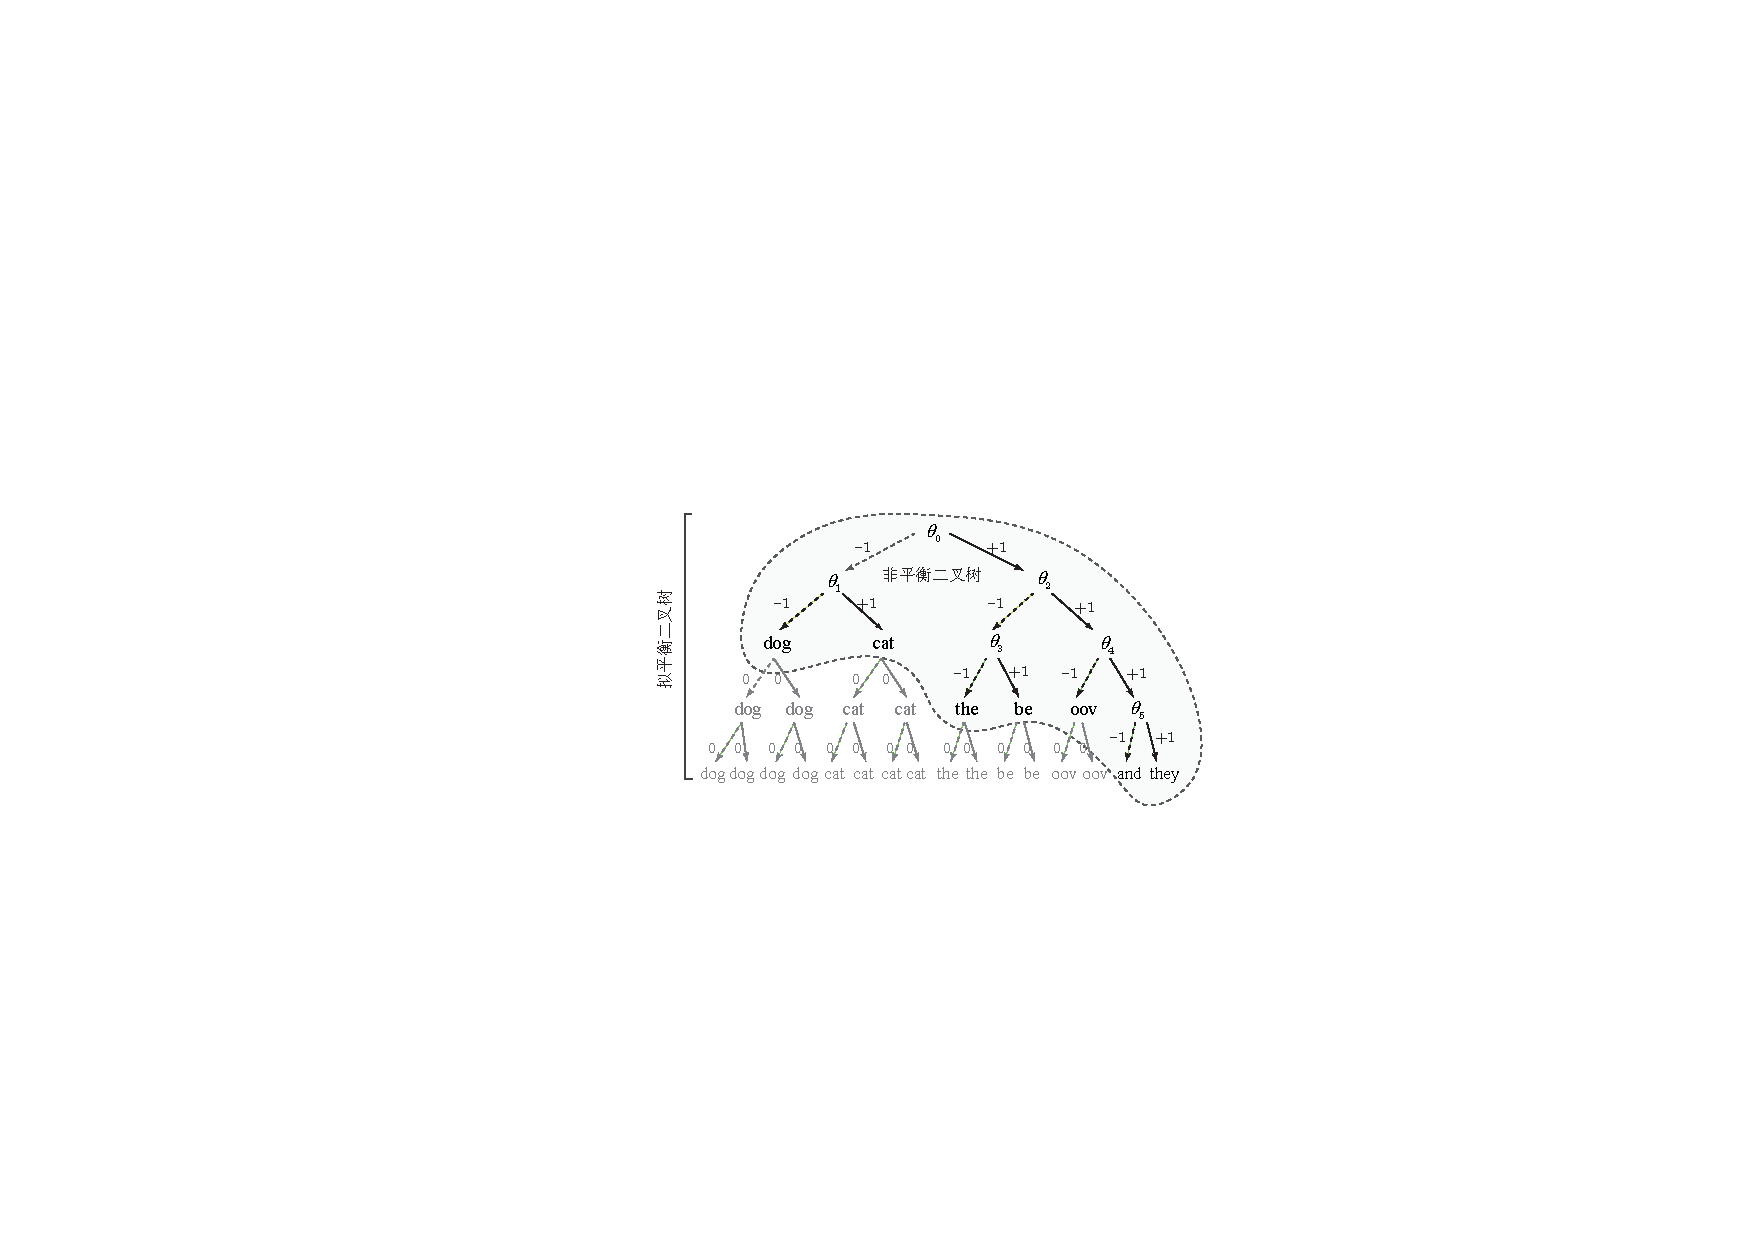
\includegraphics[width=0.85\linewidth]{./figures/thsm-example-mask.pdf}
\caption{非平衡二叉树调整成平衡二叉树}\label{fig:case_thsm_mask}
\end{figure}




除此以外,需要从矩阵$\mathcal{D}$中获得第~$w^{th}$~行向量来检索$d^w$,这里所指的$w$是词汇表中的单词索引而不是字符单词,即:$w\in [0,\mathcal{|V|}-1]$。 此外,我们需要区分模型的不同参数是在不同阶段确定的:$\{\Gamma,\mathcal{D}\}$ 是由层次聚类算法预先给定的,$\Theta$是通过训练数据集上的代价函数的梯度下降来优化的。模型实际调用的各个参数取值如表~\ref{tab:example}~所示。

\begin{table}[!h]
  \centering
  \caption{p-tHSM算法的编码和参数样例结果}\label{tab:example}
\begin{tabular}{lll}
  \toprule
  词表&路径查找表$\Gamma$& 单词路径参数\\ \midrule
dog & -1,-1,0,0,0& $\theta_0,\theta_1$\\
cat & -1,+1,0,0,0&$\theta_0,\theta_1$\\
the & -1,-1,0,0,0& $\theta_0,\theta_2,\theta_3$\\
be & -1,+1,0,0,0&$\theta_0,\theta_2,\theta_3$\\
oov & -1,+1,0,0,0&$\theta_0,\theta_2,\theta_4$\\
and & +1,+1,+1,-1& $\theta_0,\theta_2,\theta_5$\\
they & +1,+1,+1,+1&$\theta_0,\theta_1,\theta_5$\\
  \bottomrule
\end{tabular}
\end{table}

\begin{figure}[!h]
  \centering
    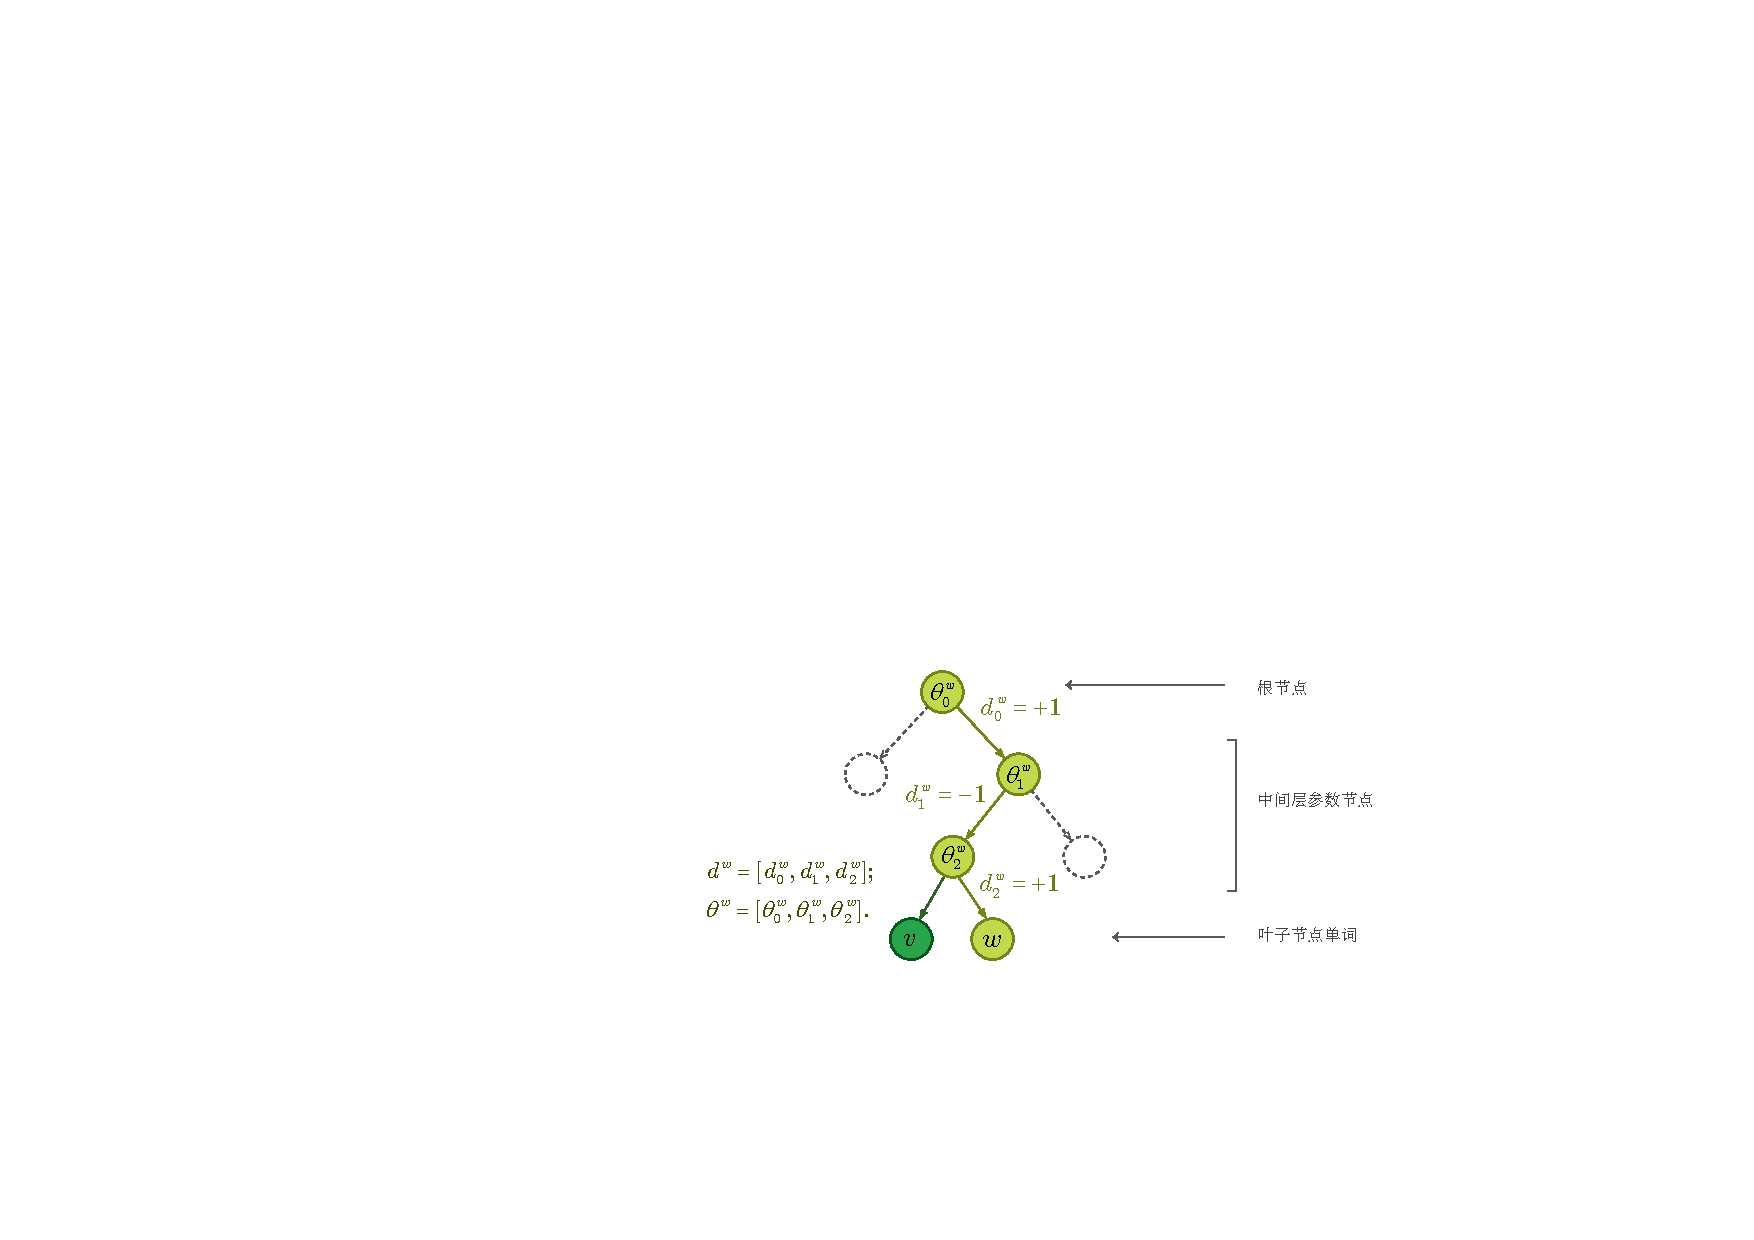
\includegraphics[width=0.93\linewidth]{./figures/thsm.pdf}
\caption{树状层次概率模型}\label{fig:tree_hsm} %
\end{figure}

\section{基于二叉树的代价函数和导数}
接下来给出模型的实际构建过程,如图~\ref{fig:tree_hsm}~所示,模型内部参数向量记为 $\theta_i^w$、 边记为 $d_i^w$,单词在树的叶子节点上。其中, 浅绿色的路径(从根节点到叶子节点~$w$)被定义为参数对 $(d^w,\theta^w)$。这里的 $d^w$ 是一个向量, $\theta^w$ 是一个参数矩阵。例如, 如图中的参数实际结果是 $d^w=[+1,-1,+1]$ , $d^{v}=[+1,-1,-1]$。

在目标词树的每个步骤中,需要对每个非叶节点是左子树还是右子树进行逻辑预测。 所以当给定$ i^{th} $节点和隐藏层的输出向量$h$的时候,可以计算标签 $d^w_i\in \{-1,1\}$的概率为:
 \begin{equation}\label{equ:pp}
\setlength{\abovedisplayskip}{10pt}
\setlength{\belowdisplayskip}{10pt}
 p(d^w_i|\theta_{i}^w,h) =\sigma(\theta_{i}^w h)^{d_i^w}\times(1-\sigma(\theta_{i}^w h))^{1-{d_i^w}},d_i^w \in [0,1]
\end{equation}
其中$ \sigma(z)= 1 /(1 + \exp(-z))$表示 $\sigma$ 函数。根据 $\sigma$ 函数的对称性规则:$\sigma(z)+ \sigma(-z)=1$,可以进一步改造和优化该公式。以下是该公式的具体证明过程如下:
\begin{equation}\label{equ:sig}
\setlength{\abovedisplayskip}{10pt}
\setlength{\belowdisplayskip}{10pt}
\sigma(z)+ \sigma(-z)  =\frac{1}{1 + \exp(-z)}+\frac{1}{1 + \exp(z)}=\frac{1 + \exp(z)}{1 + \exp(z)}=1
\end{equation}
利用$\sigma$ 函数的对称性计算规则将公式~(\ref{equ:pp})~\upcite{minka2003algorithms},缩写成:
 \begin{equation}\label{equ:upper}
\setlength{\abovedisplayskip}{10pt}
\setlength{\belowdisplayskip}{10pt}
p(d^w_i|\theta_{i}^w,h) =\sigma(\theta_{i}^w h)^{d_i^w}, d_i^w \in [-1,+1]
\end{equation}
由于公式~(\ref{equ:upper})~中的其中某一项${d_i^w}$是在指数项上面,所以我们尽管做了这个基于~$\sigma$~函数的变换,我们的计算公式仍然不是最优化的计算形式,仍然还是有空间来提升公式的紧凑性,以保证实际计算过程中的高并行度。更进一步的讲,我们可以将上面的公式缩写成以下形式:
\begin{equation}
p(d^w_i=\pm 1|\theta_{i}^w,h) = \sigma({d_i^w}\theta_{i}^w h)
\end{equation}
我们将指数项移到~$\sigma$~函数计算内部,上述计算公式就是我们所需要用到的计算形态。经过这样的操作之后,我们就完成了单节点概率计算的紧凑表示。针对计算一个单词的概率,我们需要考虑从根节点到该单词叶子节点的所涉及的所有层的概率公式。然而因为在训练的时候,我们实际上预先知道每个单词所对应的路径,所以我们实际上可以同时的计算各个节点的概率值,然后将所有节点相乘起来。这样做的好处将在后续章节进行详细说明。通过以上的操作,虽然在一定程度上增加了计算的复杂度,但是这使得后续在解决计算公式和实际运算流程之间实现一个高效的并行计算成为可能。

因此,对于我们softmax函数计算的单词的条件概率,在这里指的是:单词~$w$~在二叉树上的路径搜寻的概率,即从根到相应叶节点的路径概率$(d^w,\theta^w)$的联合乘积。具体计算公式如下所示:
\begin{equation}\label{equ:pw}
\setlength{\abovedisplayskip}{10pt}
\setlength{\belowdisplayskip}{10pt}
\begin{split}
 \log p(w|h)=&\log\prod_{i=0}^{l^w-1} p(d^w_i|\theta_{i}^w,h) \\
 =& \sum_{i=0}^{l^w -1} \log\sigma(d_i^w \theta_{i}^w h)\\
 =&\log\sigma({d^w}^\top \theta^w h)\\
 =&\zeta(- {d^w}^\top \theta^w h )
 \end{split}
\end{equation}
其中 $\zeta(z)$ 代表的是 softplus 函数: $\zeta(z)= \log (1+\exp(z))$。 该函数的导数是 $\sigma$ 函数~\upcite{DBLP:conf/nips/DugasBBNG00}, 其导数计算公式是:
\begin{equation}\label{equ:zeta}
\setlength{\abovedisplayskip}{10pt}
\setlength{\belowdisplayskip}{10pt}
\begin{split}
\frac{\mathrm{d}\zeta(z)}{\mathrm{d} z}=\frac{\exp(z)}{1+\exp(z)} =\frac{1}{1+\exp(-z)} =\sigma(z)
\end{split}
\end{equation}
如图~\ref{fig:soft}~所示, softplus 函数通常被视为 修正线性单元(Rectified Linear Unit,ReLU)的替代函数,因为他们两个函数除了零点附近分布不一样以外,其他地方分布相同。ReLU函数的计算公式为:$\mathtt{ReLU}(x)=\max(0,x)$。但是softplus函数在零点附近可导,ReLU函数在零点附近不可导。ReLU被使用的更多,因为它能获得近似线性的参数表示,这样能防止模型学习出复杂的表示,缓解模型过拟合问题。
\begin{figure}[!ht]
  \centering
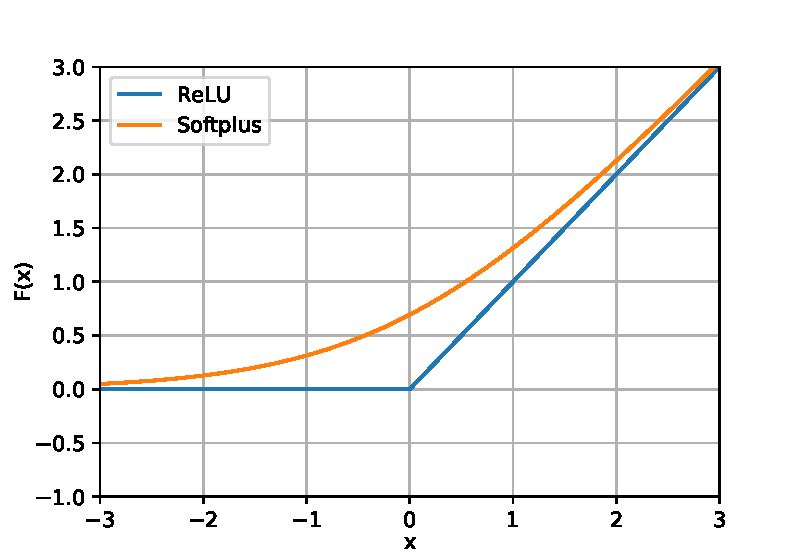
\includegraphics[width=.65\linewidth]{./figures/relus.pdf}
\caption{Softplus和ReLU函数的示意图}\label{fig:soft}
\end{figure}

前面我们已经介绍完模型的单词概率计算公式,接下来我们给出模型相应的损失函数$ \ell(\theta | h,w)$,它是定义在二叉树上面的负对数似然函数(Negative Log-Likelihood,NLL),也可以看作是所有单词概率对数误差的平均值:
\begin{equation}\label{equ:cost}
\setlength{\abovedisplayskip}{10pt}
\setlength{\belowdisplayskip}{10pt}
\begin{split}
   \ell(\theta|h,w) =&-\log\prod_{i=0}^{l^w -1} \sigma(d_i^w \theta_{i}^w h) \\
   =& -\log \sigma({d^w}^\top \theta^w h)\\
    =& \log (1+\exp(- {d^w}^\top \theta^w h )) \\
    =&  \zeta(- {d^w}^\top \theta^w h )
\end{split}
\end{equation}
从此推导公式中,我们可以发现:最小化基于二叉树的负对数似然值,意味着直接最大化softplus损失和下一个单词的分布。

接下来比较传统tHSM算法和我们推导获得的p-tHSM算法的异同点。在传统的tHSM算法中,该模型逐层计算每个节点的对数概率。 因此,这个词的整体联合对数概率通过各层线性相加。 从而,tHSM算法的时间复杂度为$\mathcal{O(|H|\log|V|})$,其计算公式为:
\begin{equation}\label{equ:cost2}
\setlength{\abovedisplayskip}{10pt}
\setlength{\belowdisplayskip}{10pt}
\ell(\theta|h,w) =\sum_{i=0}^{l^w-1} \{(1-d'^w_i)\log (\sigma(\theta_{i}^w h))  + {d'^w_i}\log (1-\sigma (\theta_{i}^w h))\}
\end{equation}
其中 $d'^w_i\in \{0,1\}$。我们可以更加形象化的理解这个函数的计算过程:这两个部分对数概率误差从二叉树的叶子底部到根节点,分别对每一层的内部节点的左右子树的联合概率进行合并,其实就是在模仿层次聚类函数从底到顶的合并节点过程。

从公式~(\ref{equ:cost2})所描述的tHSM模型和公式~(\ref{equ:cost})所描述的p-tHSM模型二者计算公式不同,我们可以分析出这两个算法的的主要区别在于:1)tHSM~算法涉及许多微小的矩阵乘法操作,而在~p-tHSM~算法中我们直接将所有参数$(d^w,\theta^w)$ 2D矩阵是以运行时内存消耗为代价的来提高模型单位时间的计算量,我们转而考虑这个向量和相对较大的矩阵的乘法,如图~\ref{fig:tree_hsm}~所示; 2)除了我们的~p-tHSM~模型的损失函数更加紧凑之外,这条路径上所有节点的对数概率而不是逐层计算而是并行的计算,为~p-tHSM~模型提供更好的时间效率。

当计算完模型的代价函数后,我们就需要计算模型的参数的导数。接下来,模型的所有参数$\{\theta^w,h\}$针对模型的代价函数的导数是 :
\begin{equation}
\setlength{\abovedisplayskip}{10pt}
\setlength{\belowdisplayskip}{10pt}
\begin{split}
\frac{\partial \ell}{\partial \theta^w}=&(\sigma({d^w}^\top\theta^w h) -1){d^w}^\top h \\
\frac{\partial \ell}{\partial h}=&(\sigma({d^w}^\top \theta^w h) -1){d^w}^\top \theta
\end{split}
\end{equation}


在这个模型中,我们采用二叉树分解的方法,主要是考虑到它一个优点是:它避免了在整个词汇表中计算概率的归一化,因为二叉树中所有的单词的总概率自然等于1。
\begin{equation}
\sum_{w\in \mathcal{V}}{p(w|h)}=\sum_{w \in \mathcal{V}}\sum_{i=0}^{l^w-1}{\sigma(d_i^w\theta_{i}^w h)}=1.
\end{equation}



\section{基于二叉树的推理算法}
接下来我们介绍,在推理阶段层次概率模型所需要解决的主要问题。
\subsection{语句打分任务}
首先,考虑到本章开始提出的第一个问题,即给定序列$ [w_1,\cdots,w_T] $,求该序列出现的概率$   \log p(w_1,\cdots, w_T)$? 直观地说,当给定相应的上下文$ h $时,我们可以通过获取一个特定单词$ w $的概率或对数概率来分解问题:
\begin{equation}
\setlength{\abovedisplayskip}{10pt}
\setlength{\belowdisplayskip}{10pt}
\begin{split}
    p(w|h) =&\sigma({d^w}^\top \theta^w h)\\
   \log p(w|h) =& -\zeta(- {d^{w}}^\top \theta^{w} h )
\end{split}
\end{equation}
其中概率$ p(w|h)$和对数概率$\log p(w | h)$可以直接通过公式~(\ref{equ:pw})~和~(\ref{equ:cost})~逐步计算出来。

因此,我们可以推导出这个序列的概率为:
\begin{equation}
   \log p(w_1,\cdots, w_T)=\sum_{t=1}^T\log p(w_t|h_t) = -\zeta(- {d^{w_t}}^\top \theta^{w_t} h_t )
\end{equation}
显然,这种类型的操作比传统的softmax方法有效得多,因为它只需要~$\mathcal{O}(\mathcal{|H|\log|V|})$~计算复杂度,而传统的softmax算法却需要~$\mathcal{O}(\mathcal{|H||V|})$。

\subsection{单词排序任务}
关于第二种情况(也被称为求解~$\arg\max$~问题),即当给定一个上下文信息时,在整个词表中搜索最有可能的下一个词(概率最大的单词)。这里的上下文可以指前文、后文或者前后文的窗口。在本实验中,我们所采用的语言模型的情况下,所指代的是前文。

在选择最佳的候选单词之前,词表中所有单词的概率可以被首先计算出,然后将他们按照概率数值大小做排序,获得所有单词的顺序结果。虽然这个过程求解的是全局最优解,但是仍然是相对缓慢的,其计算时间复杂度是~$\mathcal{O}(\mathcal{|V|})$,它涉及到遍历整个词表的二叉分层树。如在算法~\ref{alog:global}~中所描述的,为了避免两个小概率的精确度损失问题,我们选择计算每个内部节点的对数概率。


如果不采用全局最优搜索算法,而是用局部贪心算法搜索次优结果,那么计算速度能有效提升。具体来说,对于第~$i$~层中的节点,当~$p(d^w_i|\theta_{i}^w,h)\ge 0.5$~时选择左边的子树,相反的情况下选择右子树,如算法~\ref{alog:greed_argmax}~所示。因此,该策略的时间复杂度是~$\mathcal{O}(\log\mathcal{|V|})$。

\begin{algorithm}[!ht]
\SetAlgoLined
\KwData{隐藏层输出 $h$;}
 路径列表 $\mathtt{words}$=[] \;
{// 全局概率计算函数}\;
\For{$\theta_w,d_w \in \Gamma(w)$ }{
{$ \log p(w|h)=\zeta(- {d^w}^\top \theta^w h )$}\;
{words.append($\log p(w|h)$)}\;

}
{$\hat w=\arg\max_w{\mathtt{words}}$}\;
\KwResult{ 预测的单词 $w$. }
\caption{全局单词最优算法}\label{alog:global}
\end{algorithm}

\begin{algorithm}[!ht]
\SetAlgoLined
\KwData{隐藏层输出 $h$;}
 路径列表 $\mathtt{route}$=[] \;
 {// 逐层贪心路径搜索}\;
\While{$k \le \log \mathcal{V}$ }{
\eIf{$p(d_{k} |\theta_{k},h) \ge 0.5$ }{
{ $k=  k*2$// 访问左分支}\;
}{
{// 访问右分支}\;
 $k = k*2+1$\;
}
{$\mathtt{route}$.add($k$)// 将 $k$ 添加到路径列表}\;
}
$w=\Gamma(\mathtt{route})$// 通过查找$\Gamma$路径表,找出对应的单词\;
\KwResult{ 预测的单词 $w$. }
\caption{逐层贪心搜索算法\label{alog:greed_argmax}}
\end{algorithm}



\section{基于二叉树的聚类算法}
词汇表中每个单词的极性编码~$(d^w,\theta^w)$~与二叉树的结构密切相关,因此对于提出的p-tHSM算法,我们采用了多种树聚类算法来初始化单词在二叉树上的分布,以提高模型的精确性和稳定性。总的来说,这些聚类算法为每个单词生成二进制前缀字符串,表示在树中单词的路径位置,并将用于初始化p-tHSM模型。


1)一元单词聚类算法。它根据文本中单词的词频对单词进行排序,并将词频当作权重从底端到顶端进行合并,该算法也称为霍夫曼编码(Huffman Encoding)~\upcite{DBLP:conf/nips/MikolovSCCD13},算图~\ref{code:huffman}~展示了构造霍夫曼树的过程~\upcite{牛雪婷2009Huffman}。如图~\ref{fig:zipf}~所示,我们算法中用到输入信息~$\texttt{freq}$~指的是单词的词频分布,XY基坐标都是对数坐标。


\begin{figure}[!ht]
  \centering
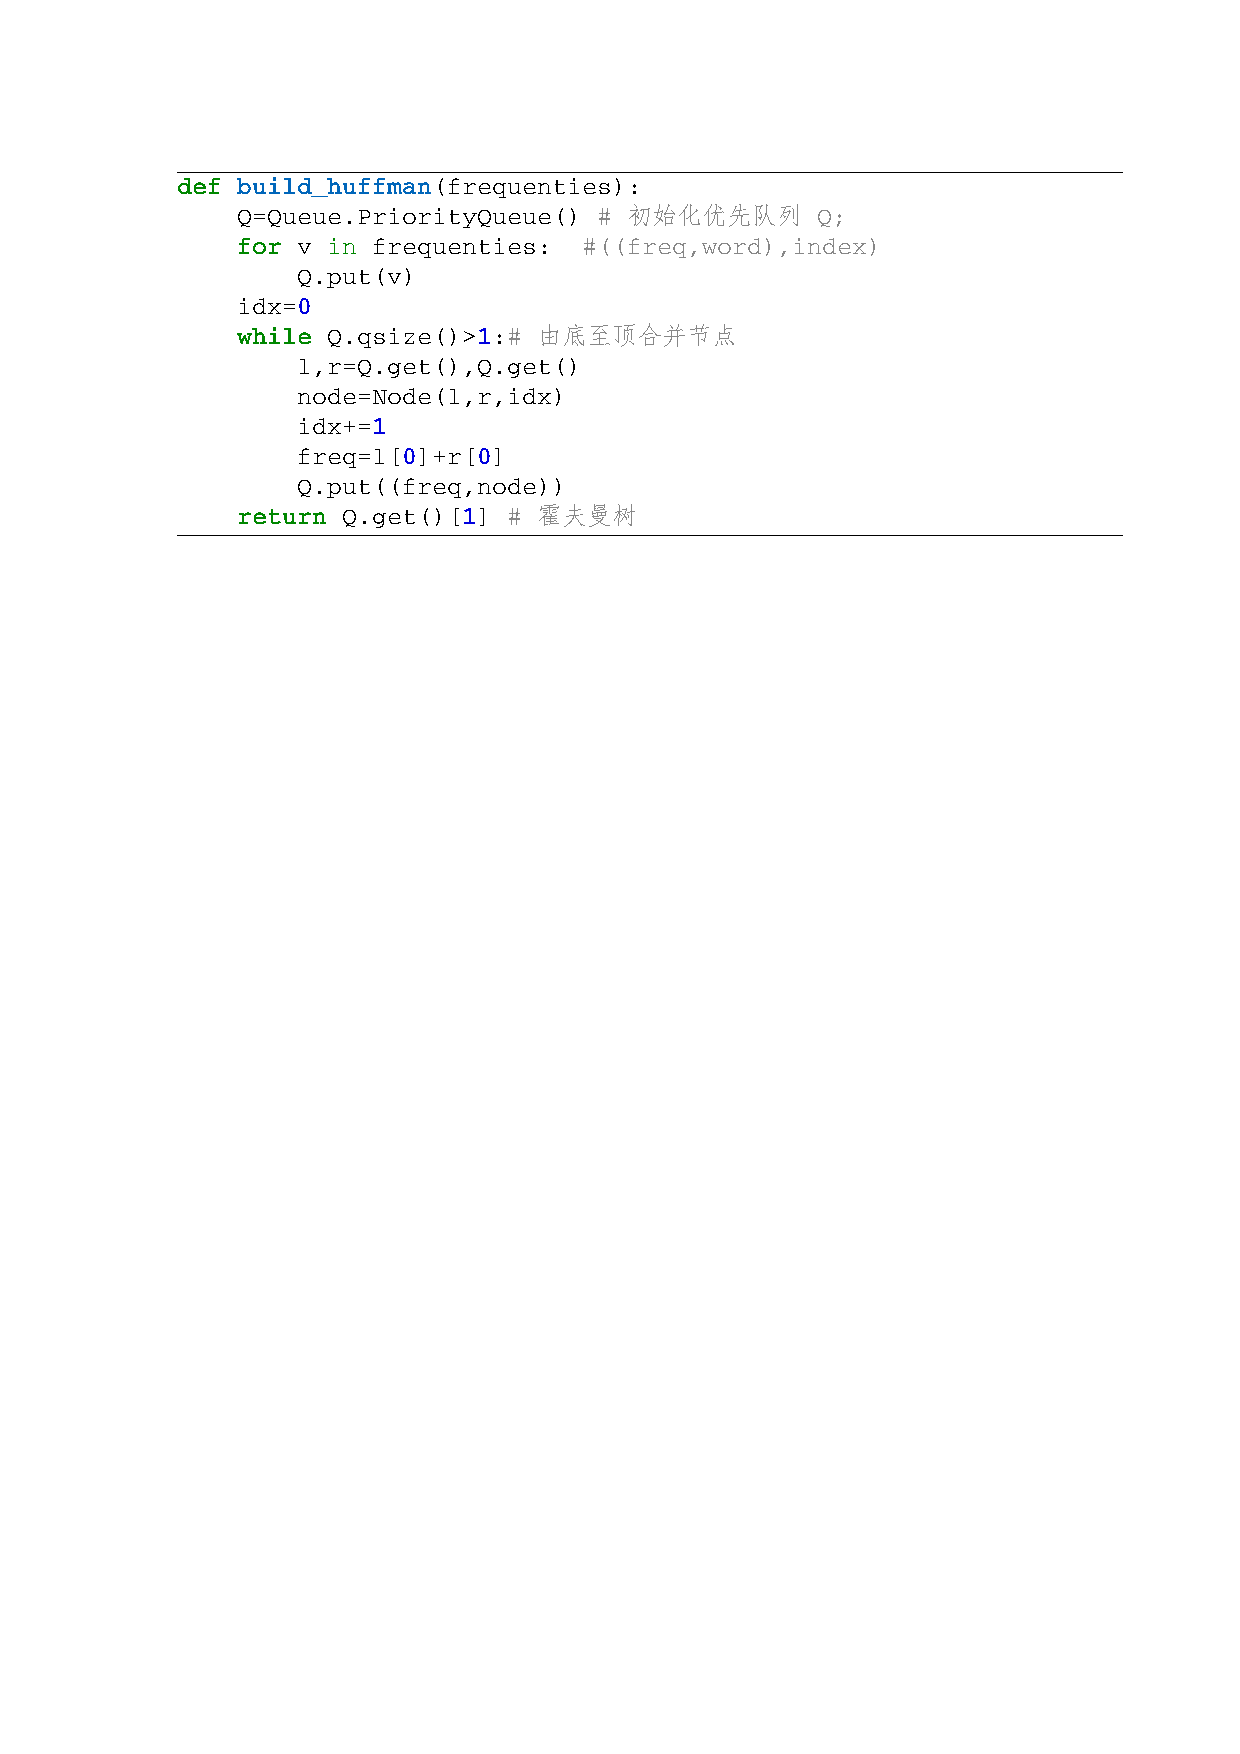
\includegraphics[width=1\linewidth]{./figures/huffman.pdf}
\caption{基于单词频率的霍夫曼建树策略}\label{code:huffman}
\end{figure}

\begin{figure}[!ht]
  \centering
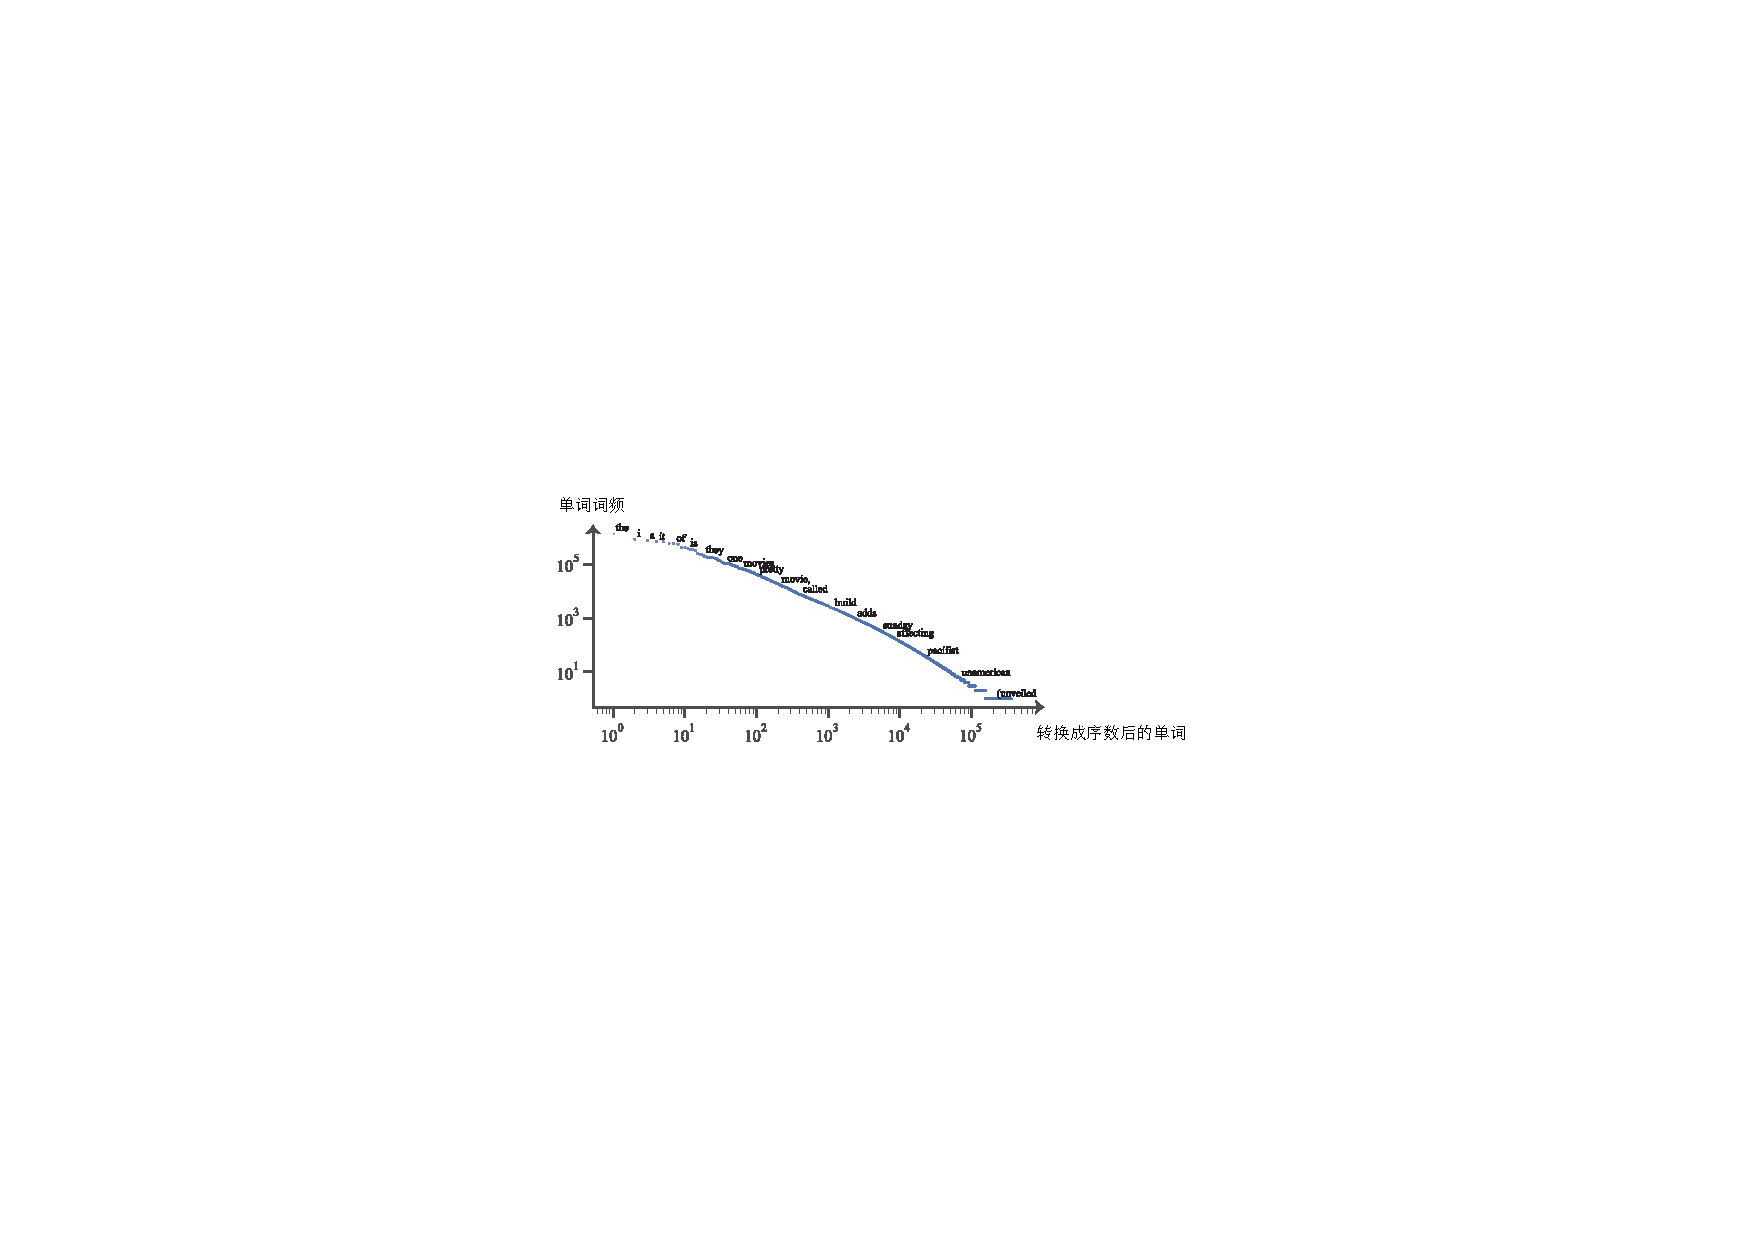
\includegraphics[width=0.85\linewidth]{./figures/zipf.pdf}
\caption{单词词频对数线性分布示意图}\label{fig:zipf}
\end{figure}

当我们构造完霍夫曼二叉树后,我们需要遍历这棵树来获取所有单词的极性编码。1) 首先我们计算待压缩数据中所有的字符及其出现次数,根据次数的不同对每个单词分配不同的权值(一般用出现频率/总字符数); 2) 其次对所有单词按其权值构造一颗霍夫曼树; 3) 对这棵树所有子树的左支用~$-1$~编码,右支用~$+1$~编码。每个位于叶子节点的字符的编码为从根节点到该叶子节点路径上的~$-1,+1$~编码值,这个在树上重新得到的编码称为霍夫曼编码。具体遍历过程可以参考图~\ref{code:preorder},算法的输出单词路径查找表~$\Gamma$~就是我们需要提前准备的单词的极性编码。


\begin{figure}[!ht]
  \centering
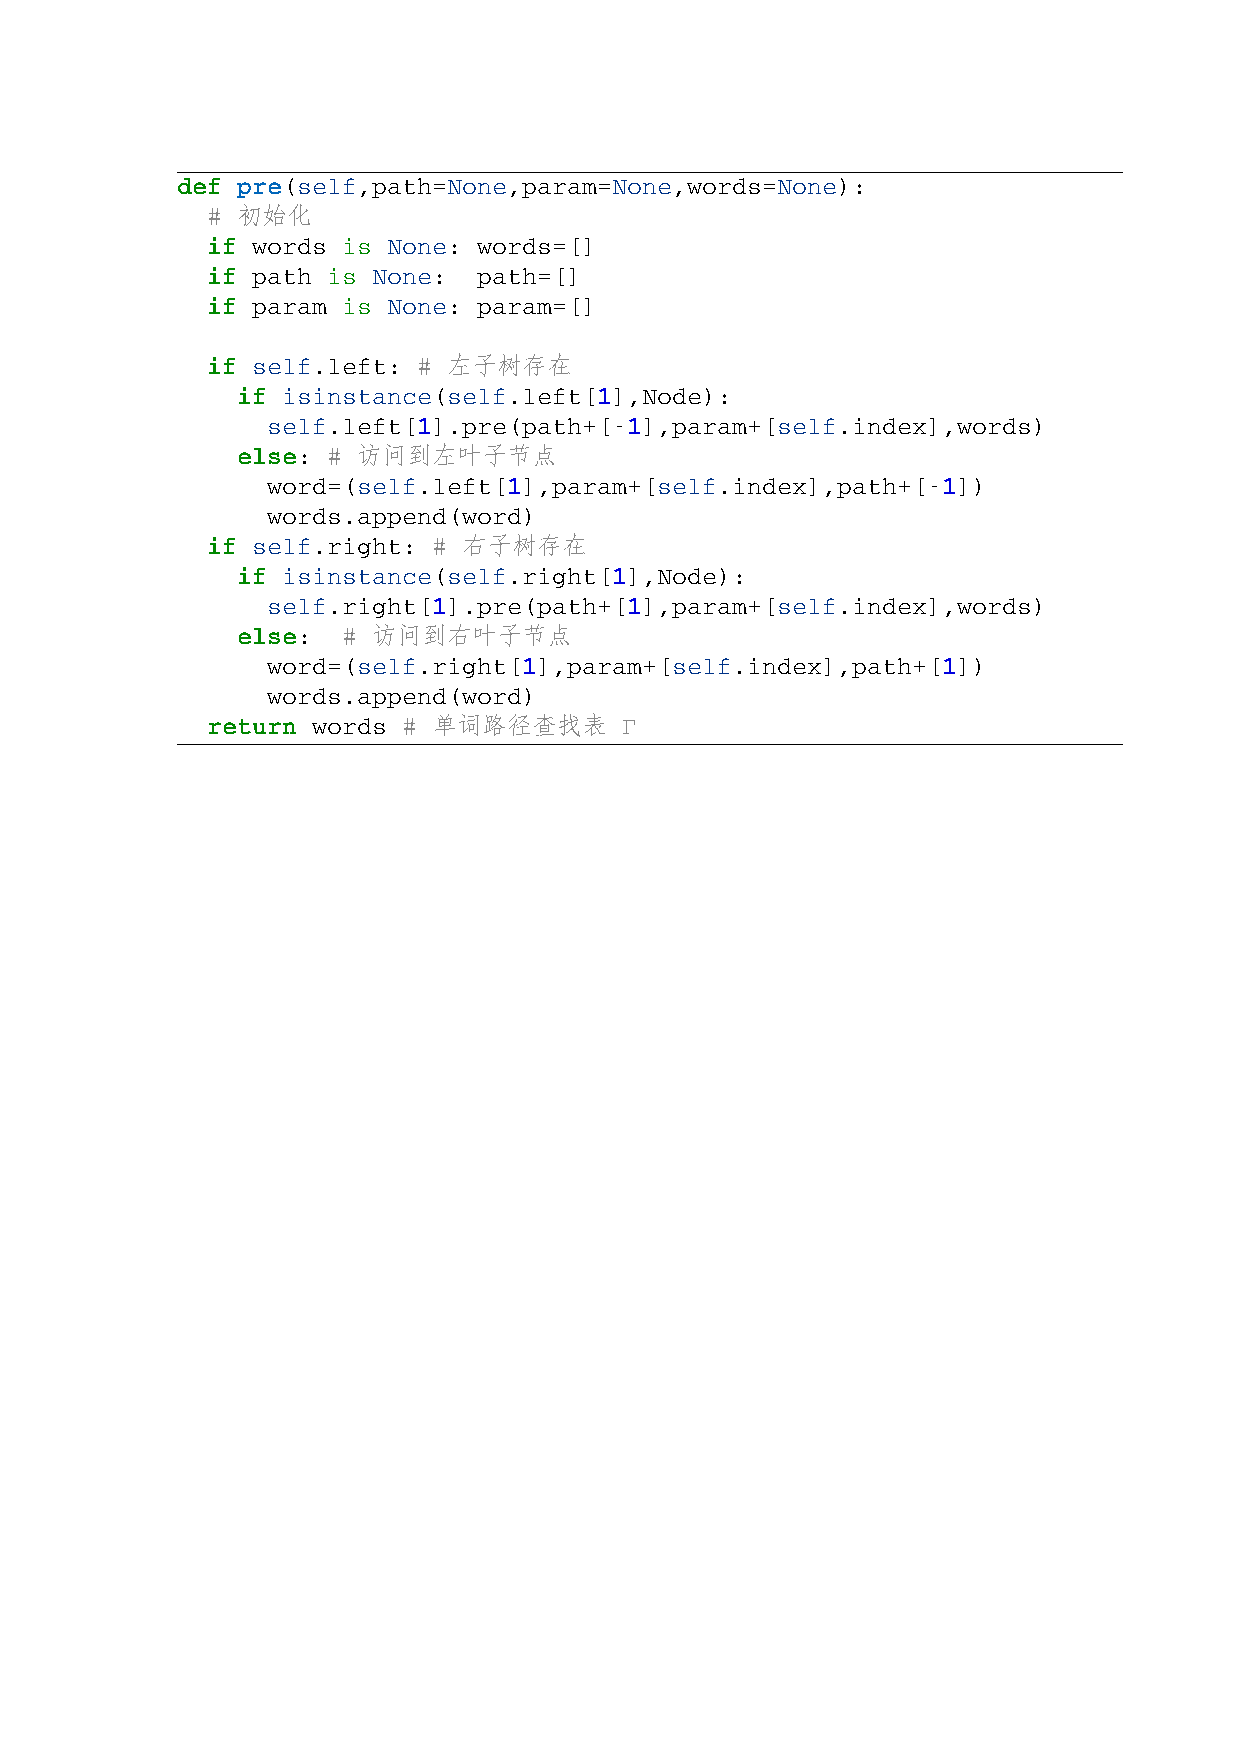
\includegraphics[width=1\linewidth]{./figures/preorder.pdf}
\caption{前序遍历函数生成单词路径查找表}\label{code:preorder}
\end{figure}

\begin{figure}[!h]
  \centering
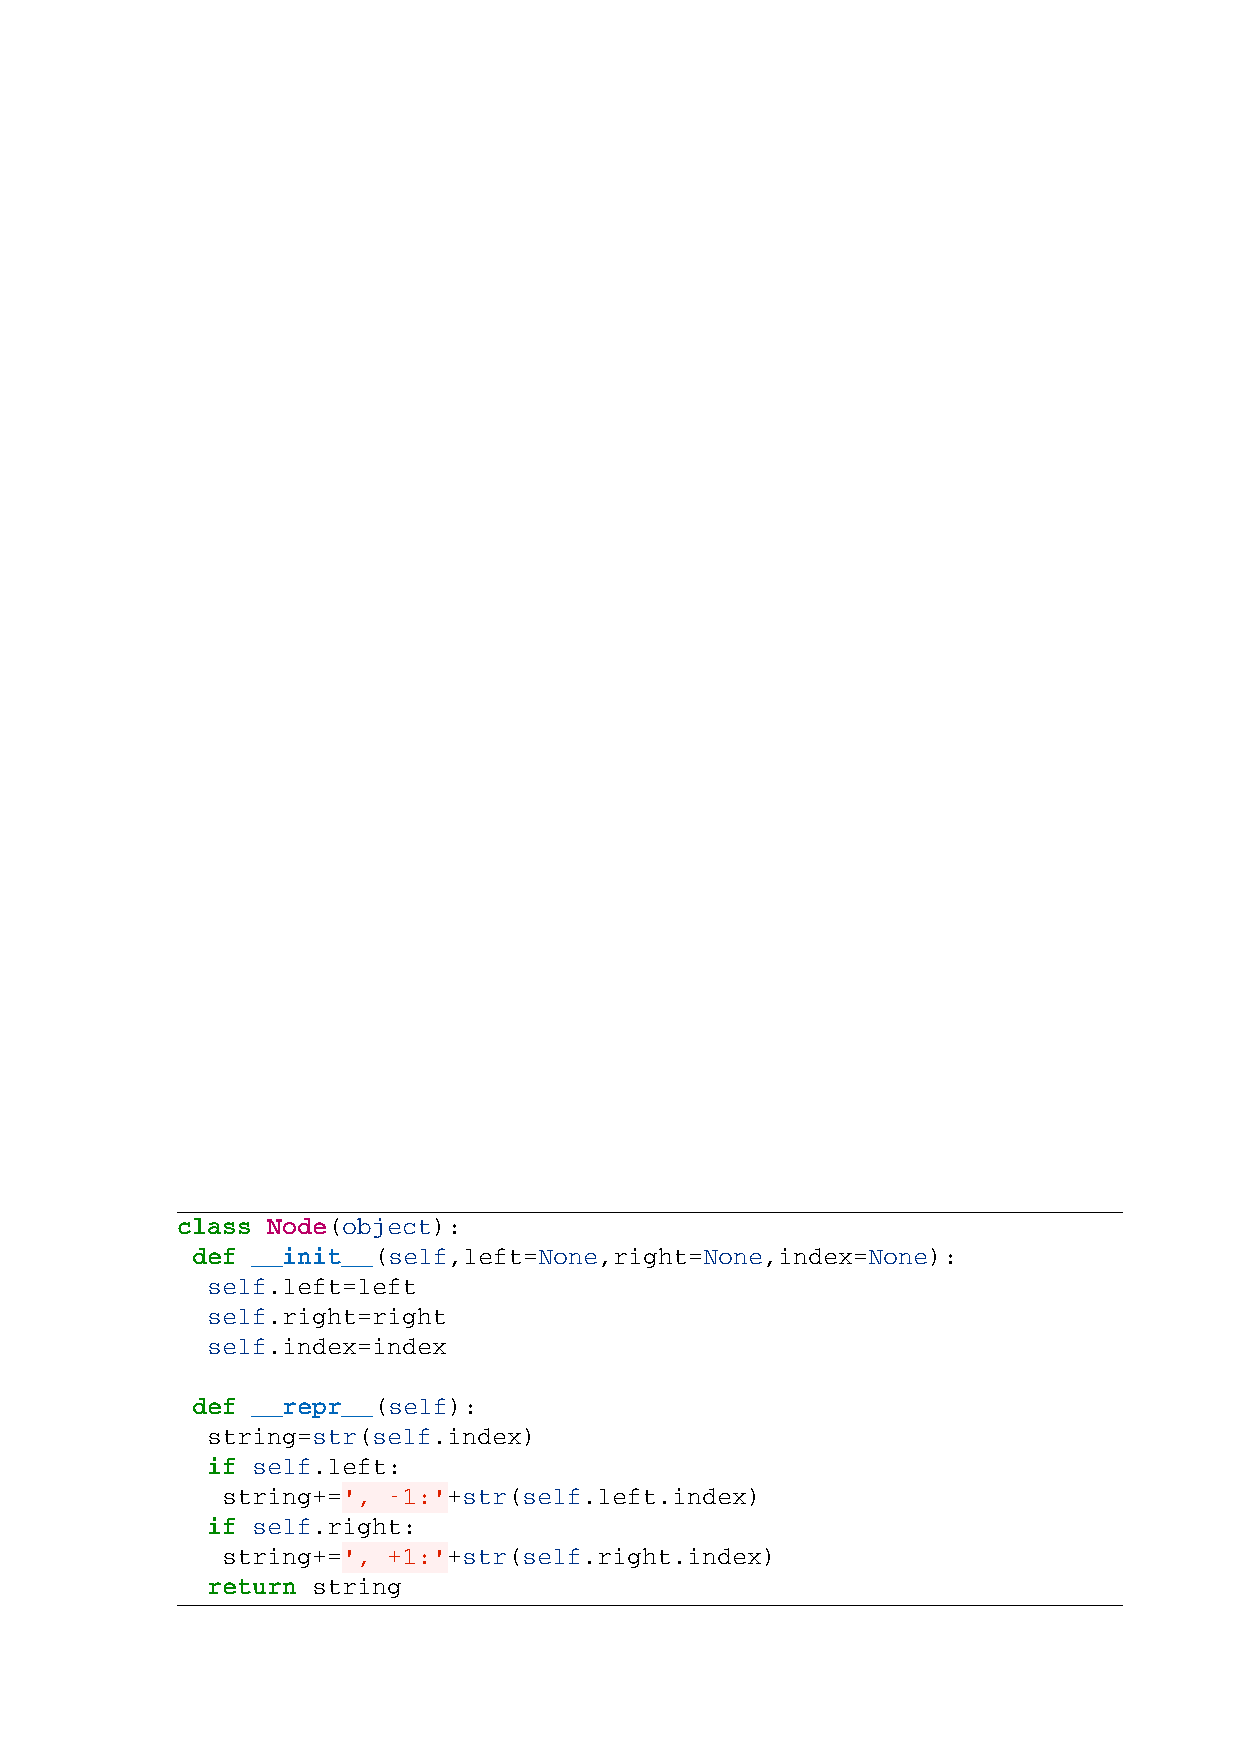
\includegraphics[width=1\linewidth]{./figures/node.pdf}
\caption{基于邻接表的二叉树节点数据组织结构}\label{fig:node}
\end{figure}

上述算法所涉及的模型的各层的节点的实际数据结构如上所示,我们采用邻接表的方式实现。其对应的二叉树的数据结构采用基于数组的方式管理和访问。如图~\ref{fig:node}~所示,每个节点(Node)包含信息为:左子树,右子树和节点编号。同时我们还定义了节点的打印字符串函数(即``\_\_repr\_\_''),方便我们检查数据结构是否正确实现。



2)二元聚类算法\footnote{https://github.com/percyliang/brown-cluster}。它也是一个由底至顶的层次聚类算法,使用Bi-gram上下文信息来确定单词的分布相似性,将相似的单词放置在二叉树的附近位置~\upcite{DBLP:journals/coling/BrownPdLM92,liang2005semi}。算法主要的计算代价就是在于初始化的时候,算法需要计算两两单词之间的距离,对于大词表来说,不断统计~Bi-gram~概率和不断计算两两单词距离是非常费时的。在将簇大小指定为~1~之后,它从底部到顶部合并具有一个节点的单词,生成的单词路径正是二叉树结构的分布.%样例如下图~\ref{fig:brown}~所示。


3)语义信息聚类算法\footnote{https://code.google.com/archive/p/word2vec/}。这种聚类算法与上面的算法非常相似,其差异点就是:该算法使用单词间的距离尺度是语义向量的余弦相似度(Cosine Distance)。我们需要先调用~Word2vec~或者~Fasttext\footnote{https://github.com/facebookresearch/fastText}~生成所有单词的词向量,然后再初始化两两单词间的距离矩阵。我们需要看到这里的问题是语言模型的其中一个任务也是生成词向量,所以这个操作可以不断自身迭代来提升最后的模型的效果~\upcite{DBLP:books/sp/mining12}。


\section{本章小结}
本章首先定义了极性编码的概念,同时给出了模型所涉及的参数的详细含义。接下来逐步推导模型的单个节点的概率公式,单个词的概率公式和模型的代价函数。另一方面,我们将提出的p-tHSM算法和传统的线性~tHSM~算法进行的比较,通过对比两者计算的差异性证明我们提出的算法具有更高的计算吞吐量,速度更快。
因为基于二叉树的概率计算方案和传统的softmax计算方案不同,不能直接输出单个词的概率或者计算最佳的候选单词,我们进一步还讨论了模型在测试的时候所需的推理算法,所以我们分别针对排序和打分两个任务提出相应的策略。
最后,由于单词在二叉树上的分布需要初始化,我们概述了传统的霍夫曼聚类算法、布朗聚类算法和语义向量聚类算法。


%\RestyleAlgo{boxed}
\chapter{类别层次概率计算模型}
上一章介绍了将预测端的词用二叉树的分层的形式表示,本章将这个目标词表示扩展到类别的形式,并讨论基于类别划分的层次概率模型。首先本章提出在划分的类别结构上建模的单词编码方案,进而推导出该模型的代价函数及其梯度。同时在实验中注意到类别划分的单词分布对模型的性能有很大的影响,应需要在训练阶段之前被定义,所以本文考虑几种现有的词表分割策略,包括:基于单词或者文本的统计、句法和语义知识来划分其层次结构,使模型能达到稳定和高效的结果。在模型推理过程中,本章针对两种不同的情况:1)打分:输出给定序列的概率;2)排序:在给定的上下文中获取得分最高的候选单词,分析并提出可能的优化策略。


\section{词表划分编码}
\begin{table}[!ht]
  \centering
  \caption{类别层次概率计算模型的符号助记表}
\begin{tabular}{llc}
  \toprule
   符号&含义&取值范围\\ \midrule
$\theta^c\in\mathbb{R}^m$ &表示单词的类别向量& Float32\\
$ \theta^o$ &表示路径$l^w$表示划分后的单词三维张量&Float32 \\
$\Gamma'$ &路径查找表,给定单词元组序列,可以获得对应的单词&--- \\
  \bottomrule
\end{tabular}
\end{table}
词表分割算法能将词表划分成多个大小不均匀的分组,传统的类别层次模型仅能计算均匀划分后的单词概率,为了支持广义的词表划分算法,本章提出基于词表划分的元组编码方式。

首先介绍非均匀划分的词表的编码方式,词表被表示成:类别向量~$\theta^c$~和划分的单词矩阵~$\theta^o$。其中前者定义了类别层的概率~$p^c$~,而后者表示该分组内的单词局部概率~$p^o$,如图~\ref{fig:unequal}~所示。其中,划分的单词矩阵的维度是:类维度和分组词维度。如果将词表~$\mathcal{V}$~划分为不等大小的组,则需要将单词矩阵分类为等长矩阵,对于不在这个组中的剩余节点,我们使用零掩码~$\theta^m$来消除其对局部单词概率和总代价函数的影响。
因此,分组词维度是最大的组长度。如果应用词表均匀分割的算法(如图~\ref{fig:equal}~所示),掩码向量~$\theta^m$~可以被忽略,并且分组词维度是~$\mathcal{|V|/|C|}$(~$\mathcal{|C|}$~表示类维度)。另外,如果~$\mathcal{|V|}$~不能被~$\mathcal{|C|}$~整除,那么最后的分组包含实际的单词数量应该小于该组的大小。考虑到这样的不存在的单词占据很少一部分,同时不影响其他类别的概率计算,实际的影响比较小,所以掩码向量~$\theta^m$~可以被忽略。
\begin{equation}\label{equ:partition}
 \theta^m=
\begin{cases}
    \text{单位矩阵,}& \text{若均匀划分} \\
    \text{掩码矩阵,} & \text{否则}
\end{cases}
\end{equation}

\begin{figure}[!ht]
  \centering
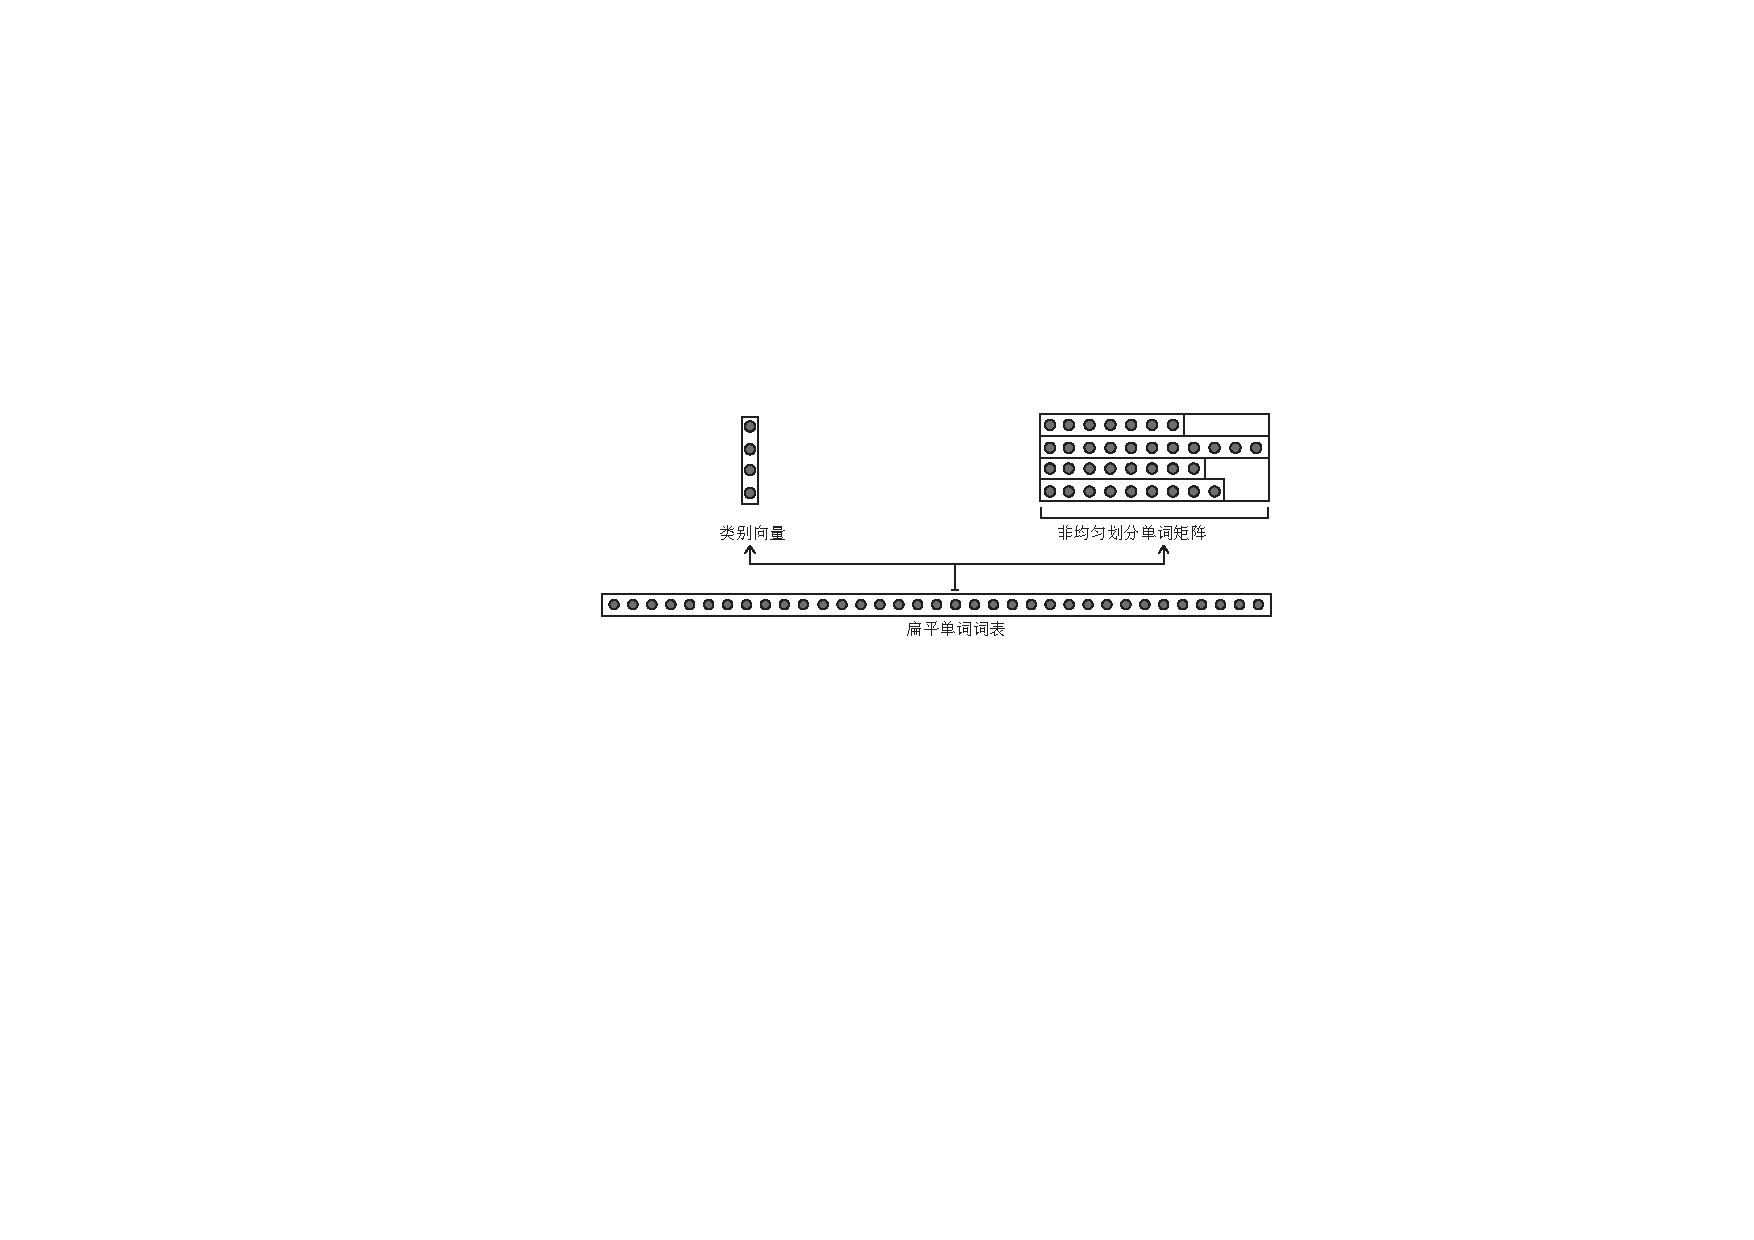
\includegraphics[width=.9\linewidth]{./figures/chsm-simple.pdf}
\caption{非均匀词表划分结构示意图}\label{fig:unequal}
\end{figure}
\begin{figure}[!ht]
  \centering
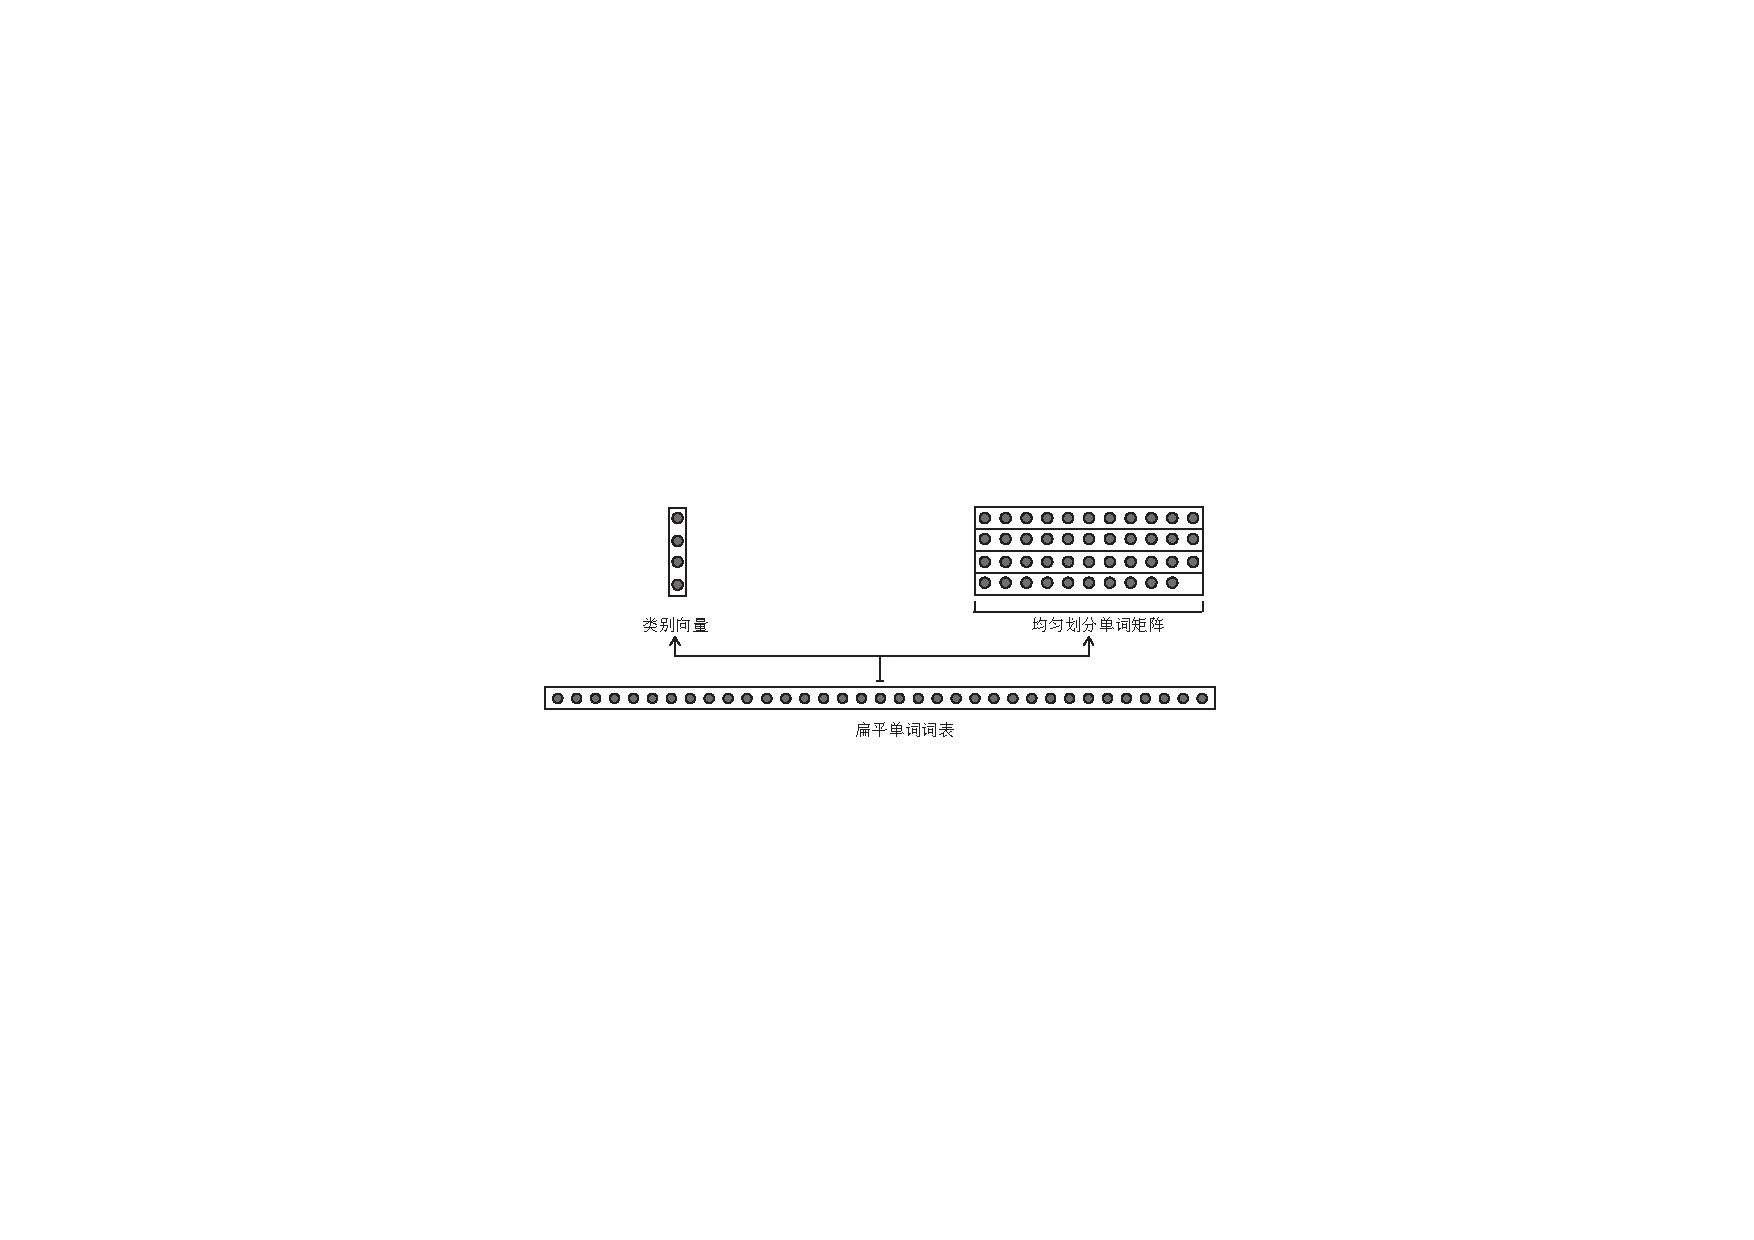
\includegraphics[width=.9\linewidth]{./figures/chsm-simple2.pdf}
\caption{均匀词表划分结构示意图}\label{fig:equal}
\end{figure}

上述的编码方式将一维~1-of-K~的单词索引替换成元组方式的索引~$(w^c,w^o)$,通过该元组可以从预先定预先定义的单词查找表~$\Gamma $~中检索给定单词~$w$,或者给定单词~$w$,通过反向的查找表给出该元组。其中~$w^c$~指代的是单词的类别编号,$w^c$~表示该组内的单词索引。这种编码方式不仅能处理传统的均匀划分词表同时也支持非均匀划分的词表结构。


\section{基于类别的代价函数和导数}
在定义单词基于类别的二元编码后,本章接下来讨论基于这种编码的代价函数和导数计算公式。
给定隐藏层输出向量~$h$,那么该分组中的每个组和和该分组中单词的局部概率可以被定义为:
\begin{equation}
\setlength{\abovedisplayskip}{10pt}
\setlength{\belowdisplayskip}{10pt}
\begin{split}
\log p^c(c|h) &= \theta^c h-\log \sum{\exp( \theta^c h )} \\
\log p^o(w|w^c,h)&=\theta^o h -\log\sum\exp{(\theta^o h)}
\end{split}
\end{equation}
其中~$p^c$~和~$p^o$~是分别计算而不是同时计算的。因为主要的计算瓶颈在单词局部概率~$p^o$~中,所以主要问题是减少第二项概率的计算量而不是同时计算这两项概率。因此本文的主要工作集中在如何高效计算~$p^o$。例如,假设我们将词表大小为~10000~的单词均匀划分,那么类别向量的维度是~100,单词矩阵的维度是~$[100,100]$。如果两者能够同时计算,而不是依次计算,它所带来的计算效率增益可以如下计算:
\begin{equation}\label{equ:example}
\setlength{\abovedisplayskip}{10pt}
\setlength{\belowdisplayskip}{10pt}
  \frac{\frac{1}{100*100}}{\frac{1}{100*100+100}}-1=1\%
\end{equation}
从上面的计算结果来看,我们只能提升~$1/\%$~的速度方面性能。那么如果每次只计算对应单词的单词矩阵的概率值,计算效率可以如下计算:
\begin{equation}\label{equ:example2}
\setlength{\abovedisplayskip}{10pt}
\setlength{\belowdisplayskip}{10pt}
  \frac{\frac{1}{100+100}}{\frac{1}{100*100+100}}-1=49.5
\end{equation}
可以发现,只要能避免计算全局概率就能实现~$49.5$~倍的计算效率增益。使用分类的层次概率模型能直接将模型的计算瓶颈削弱到很少计算时间,尽管相比于树状模型该模型的计算速度不是最快的。除此之外,基于类别的层次概率模型的优点包括:1)模型鲁棒性更强,单词的分组分布对模型的精确度影响比树状层次概率模型小;2)模型实现容易,通用性强。只需要将所有单词划分几个分组即可,不需要做层次二叉聚类算法,而且层次二叉聚类算法计算时间复杂度相当高,不适合实际使用。



在介绍完模型的类别编码方式中提及的掩码向量并不是直接应用于这个分词矩阵,而是应用在对数概率归一化(log softmax)的计算步骤中。 举例来说,在~softmax~函数中:$p(x_i)={\exp({x_i}})/{\sum_j\exp(x_j)}$,如果~$x_k=0$,然而其概率值~$p(x_k)>0$~,这是因为~$\exp(x_k)>0$。即:在该类别中不存在的单词,仍然有概率数值和概率分布,这样对于那些实际存在的单词概率来说,至多有~$\mathcal{|V|/\mathcal{C}}-1$~的类别概率被稀释,这被称为概率稀释问题。因此,该组中正确的的局部单词的对数概率计算如下:
\begin{equation}
\setlength{\abovedisplayskip}{10pt}
\setlength{\belowdisplayskip}{10pt}
  \log \tilde p^o(w|w^c,h)=\theta^o h -\log\sum\theta^m\exp(\theta^o h)
\end{equation}
其中~$\theta^m\exp(\theta^o h)$~保证了那些不存在的单词经过掩码向量之后数值是~0,从而不会对公示的第二项产生影响。

接下来推导模型的代价函数,模型的预测损失主要来自两项:类别预测错误和分组中的单词预测错误,所以该层次模型的损失函数可以从这两项错误分类中算出,可以写成如下的形式:
\begin{equation}
\setlength{\abovedisplayskip}{10pt}
\setlength{\belowdisplayskip}{10pt}
\ell(\theta|h) =\log p^c(w^c|h) +\log \tilde  p^o(w^o|w^c,h)
\end{equation}
其中计算$\log \tilde  p^o(w^o|w^c,h)$,需要指定其类别~$w^c$。在模型训练过程中,$w^c$~是需要预先定义的,在测试过程中,需要同时考虑 ~$p^c$~和 ~$p^o$~两项概率,才能选择概率最大的单词,单独计算$\arg\max p^c$~和 ~$\arg\max p^o$~均无法获得概率最大的单词。

总的来说,将词表分成相互排斥的分组的优点可以概括为:1)避免了在整个词表上计算归一化(Normalization)概率。 由于~$p^c$~是在类维度上计算概率归一化概率,$p^o$~是在最大组大小维度上计算归一化概率。 所以在第二个方程中,其他分组中的单词被忽略不需要计算,其中~$\mathcal{|C|}$~和~$\mathcal{|V|}/\mathcal{|C|}$~在最大的实验数据集都不会超过~1000; 2)与基于二叉树结构相比,它对词表的结构约束(Structural Constraint)更少,在分层预测过程中丢失的信息更少;3)与单词拆分方法相比,它不会增加序列长度,所以不会影响循环网络的长距离依赖的建模问题。

当定义模型的代价函数之后,接下来推导得模型所涉及的参数的导数,以便于模型求解优化。模型的所有的参数包括:$\{\theta^c,\theta^o,h\}$,模型的代价函数对于这些参数的导数计算公式如下:
\begin{equation}
\setlength{\abovedisplayskip}{10pt}
\begin{split}
\frac{\partial \ell}{\partial \theta^c}=& (\delta_{ij}-p(c|h))h \\
\frac{\partial \ell}{\partial \theta^o}=&(\delta_{ij}-p(w|c,h))h \\
\frac{\partial \ell}{\partial h}=&(\delta_{ij}-p^c(c|h))\theta^c + (\delta_{ij}-p^o(w|c,h))\theta^o
\end{split}
\end{equation}


\section{基于类别的测试推理}
在推理测试阶段,对于类别的层次概率模型来说,序列的概率直接运用模型的代价函数计算获得,如下所示:
\begin{equation}\label{equ:class_inf}
\setlength{\abovedisplayskip}{10pt}
\setlength{\belowdisplayskip}{10pt}
\log p(w_1,\cdots, w_T)=\sum_t^T\log p(w_t|h_t) =\sum_{t=1}^{T}\log p^c(w^c_t|h_t) +\log p^o(w^o_t|w^c_t,h_t)
\end{equation}
其计算复杂度是~$\mathcal{O(|H|\sqrt{|\mathcal{V}|})}$~,比softmax函数计算效率更高,两者的加速比是~$|\mathcal{V}|/\sqrt{|\mathcal{V}|}$。

\begin{algorithm}[!ht]
\caption{基于 cHSM 算法的全局 $\arg\max$ 算法}\label{algo:alls}
\KwData{ 隐藏层输出 $h$}
 \For{$c \in \mathcal{C}$ }{
 {// 计算类别的概率~$\log p^c(c|h)$}\;
 {$\log p^c(c|h) = \theta^c h-\log \sum{\exp( \theta^c h )}$}\;
 \For{w $\in$ c}{
 {// 计算单词的条件概率~$\log p^o(\hat w^o|\hat y^c,h)$}\;
 {$ \log \tilde p^o(w|w^c,h)=\theta^o h -\log\sum\theta^m\exp(\theta^o h)$}\;
 {// 计算每个单词全局概率}\;
  {$\log p(w|h)=\log p^c(w^c|h)+\log \tilde p^o(\hat w^o|\hat w^c,h)$}\;
 }
 }
 {$w=\arg\max_w \log p(w|h)$}\;
 \KwResult{概率最大的候选单词$w$。}
\end{algorithm}

其次对于第二种词表排序的情况,首先可以计算词汇表中所有单词的概率,然后调用排序函数,从而选择概率最高的单词,如算法~\ref{algo:alls}~所示。 此外,我们仍然可以在算法~\ref{alog:exact}~中对上述方法进行少量修改,然后计算全局概率最佳的单词。两者的差异是,算法~\ref{alog:exact}~最后的$\arg\max$的计算量是~$\mathcal{|C|}$,算法~\ref{algo:alls}~最后的$\arg\max$的计算量是~$\mathcal{|V|}$。
\begin{algorithm}[!t]
\caption{基于~cHSM~算法的贪心$\arg\max$ 算法}\label{alog:exact}
\KwData{ 隐藏层输出 $h$}
{// 挑选每个类中概率最大的单词}\;
 {$\hat w^o=\arg\max_o{\log p^o(w| c,h)}$ }\;
 {// 在这些已经被栅选单词中挑选最佳的单词}
 {$\tilde w^c=\arg\max_c{\log p^c(w^c|h)+\log p^o(\hat w^o|\hat y^c,h)}$}\;
通过查找表 $\Gamma'$ 将 $(\tilde w^c,\hat w^o[\tilde w^c])$替换成单词$w$ \;
 \KwResult{概率最大的候选单词$w$。}
\end{algorithm}


此外,cHSM算法的性能对词表划分算法有些敏感,因为某些方法可能会产生高度不平衡的字组,并且这种单词不均匀分布会在算法中产生标签偏差问题(Label Bias)。第一个本地~$\arg\max_o$~进程~\upcite{DBLP:conf/icml/LaffertyMP01}。然而,在大多数情况下,如果选择合适的参数,则可以考虑不平衡的问题,本文考虑平衡词汇分区的广义形式。

我们接下来来详细说明标签偏差问题。考虑两个类~$c_p$~和~$c_q$,这两个类的包含的单词数量是不同的,我们不妨假设~$|c_p|\le|c_q|$。在计算了最后一个隐藏层输出~$h$~与类图层参数的相似性之后,我们继续计算~$h$~与每个组的内部单词~$w$ 的相似性得分,这些单词在每个特定组中都没有进行局部规范化整个词汇。当~$|c_p|\approx|c_q|$~表示我们希望将词汇聚类成等大小的群组,而不是高度倾斜的群组分布时,可以减轻标签偏差问题,其中~$|c_p|\ll|c_q|$ 。更具体地说,对于分布不均的情况,对于类~$c_q$~中的单词来说这个概率被一大群单词稀释是不公平的,这样算法更有可能以较高的概率取出这个小组中的单词,放弃在其他大集团有更多的潜在的话。

我们可以用局部贪心算法搜索次优结果,而不是搜索确切的全局最优结果,可以将这个$\arg\max$进程分解为两个阶段:1)计算类概率,并挑选概率最大的类 $\hat c $; 2)计算该类别下的单词概率 $\hat c$,并选择具有最高局部概率的单词。这个算法会给出局部最优的单词而不是全局最优的单词,但是与原始算法~\ref{alog:exact}~相比,它的运行速度要快得多。而且,由于单词计算的是局部概率归一化,标签偏差问题可以在一定程度上缓解。在实验研究中将讨论算法~\ref{alog:exact}~和~\ref{alog:cargmax}~的详细不同性能。
\begin{algorithm}[!t]
 \caption{基于 cHSM 模型伪贪心 $\arg\max$ 算法}\label{alog:cargmax}
\KwData{隐藏层输出 $h$;}
{// 挑选概率最大的类别}\;
 {$\hat w^c=\arg\max_c{\log p^c(c|h)}$ }\;
 {$\hat w^o=\arg\max_o{\log p^o(w|\hat w^c,h)}$}\;
 {// 在这个类别下面,挑选概率最大的单词}\;
 {通过查找表 $\Gamma'$ 将 $(\hat w^c,\hat w^o)$替换成单词$w$}\;
 \KwResult{ 最佳的候选单词 $\hat w$.}
\end{algorithm}

\section{词表划分算法}
由于cHSM模型的性能与其词汇分割算法密切相关,我们将聚类算法的现有工作进行汇总,并将可能的方法分类如下:

\subsection{均匀词表划分算法}
1) 随机初始化。 这种直观的方法忽略了单词的所有外部信息,能用于揭示其他聚类方法的最坏情况,也可以揭示其他聚类策略的相对收益。

2) 字母顺序。这种方法根据字符级别的信息对单词进行排序,同一组中的单词共享一个相似的子字符串。


3) 一元单词聚类。这些单词首先根据它们在文本中的频率排序,然后对这个列表均匀划分,从而形成词频连续的单词块。这种方法具有这样的性质:编号较低的类比较高编号的类访问频率更高,因为它们的词频更高~\upcite{DBLP:conf/nips/MikolovSCCD13}。



\subsection{非均匀词表划分算法}
1) 二元单词聚类。又称为指布朗聚类方法,这是历史适用于基于N-gram的基于类的模型~\upcite{DBLP:journals/coling/BrownPdLM92,liang2005semi}。单词使用相同的Bi-gram信息将会划分到相同的行中。

2) 结构聚类\footnote{https://github.com/AlonDaks/unsupervised-authorial-clustering}。根据文本中的单词的词性和句法结构划分词表~\upcite{DBLP:conf/acl/DaksC16} 。

3) 语义聚类。我们将传统的kmeans聚类方法应用到预训练的词响亮,使得我们可以通过指定聚类的大小将词汇分成不同的形状。

\section{本章小结}
本章首先定义了基于词表划分的编码概念,同时给出了模型所涉及的参数的详细含义。接下来,为了支持词表的非均匀划分结构,我们提出了二元组的编码方式,将非均匀单词矩阵填补成均匀矩阵和对应的掩码矩阵,然后逐步推导模型的概率公式和代价函数。进一步的,我们还讨论了模型在测试的时候所需的推理算法,因为基于划分词表的概率计算方案和传统的softmax计算方案不同,不能直接输出单个词的概率或者计算最佳的候选单词,所以我们分别针对这两个任务提出推理算法。最后,由于单词在单词划分矩阵上的分布需要初始化,我们讨论了传统的霍夫曼硬聚类算法,布朗软聚类算法和语义向量软聚类算法等等。同时也讨论三种算法的实际应用过程。
%
\chapter{语言建模实验结果与分析}
前面两章分别介绍了基于树状和类别的层次概率模型的具体建模过程,本章将比较这两种分层模型与已有的算法(Baselines)在计算效率和精确性上的差异,并且在三个标准文本数据集上进行语言建模的实验研究和结果分析。
接下来将讨论分析不同层次概率算法与其他大词表问题的优化算法在单词困惑度和单词错误率上的结果对比和实验分析。除此以外,还将从效率、可扩展性、参数大小等方面对这些方法进行实验研究并作讨论分析。

\section{实验设置}
这一小节将介绍实验所需要用到的文本数据集,还有语言建模实验的两种主要的评测指标和实验模型的实际参数配置和训练过程。
\subsection{实验数据集}
本实验所采用的数据集主要是依照两个目的选取:1)首先为了便于实验复现和互相对比,需要在小数据集上反映出参数变化对模型最后的性能产生的影响;2)同时还需要在大数据集上展示模型参数在最佳参数配置下,比较模型之间的最优结果的差异点。
所以本实验选取了三个标准文本数据集:Wikitext-2,Wikitext-103 和 One Billion Words(OBW)数据集。
如表~\ref{tab:dataset}~所示,表中列举了这三个数据集的相关统计指标,包括:单词数量、句子数量、词表大小和词表外单词的比例(Out-of-Vocabulary,OOV)。需要注意的是词表大小不能改变,因为不同词表规模的模型之间理论上就不在同一个基准之上,其次是由于模型的一个的评测指标和词表大小成负相关关系,所以表~\ref{tab:dataset}~中展示的数据已经预先固定不会再做任何的修改,例如:不能对数据集做单词大小写变化、数词转换操作或者分词操作。
\begin{table}[!ht]
  \centering
  \caption{WikiText-2、WikiText-103 和 One Billion Words 数据集统计指标 \label{tab:dataset}}
\begin{tabular}{llrrrrr}
\toprule
数据集& 类型& 文章数量  & 句子数量 & 单词数量 & 词表大小 & OOV(\%) \\ \midrule
\multirow{3}{*}{Wikitext-2} &训练集& 600 & 36,718 & 2,088,628 & \multirow{3}{*}{33,278} & \multirow{3}{*}{2.6\%} \\
&验证集& 60 &3,760 & 217,646  & &\\
&测试集& 60 & 4,358 & 245,569 & &\\
\midrule
\multirow{3}{*}{Wikitext-103} &训练集& 28,475 &  1,801,350 &  103,227,021 & \multirow{3}{*}{267,735} & \multirow{3}{*}{0.4\%} \\
&验证集& 60 &3,760 & 217,646  & &\\
&测试集& 60 & 4,358 & 245,569 & &\\
\midrule
\multirow{3}{*}{One Billion Words} &训练集& --- &30,301,028&768,646,526&   \multirow{3}{*}{793,471} &   \multirow{3}{*}{0.28\%} \\
 &验证集& --- &  6,075 &   153,583 &&\\
 &测试集 & --- &  6,206 &   159,354 &&\\
\bottomrule
\end{tabular}
\end{table}

Wikitext-2~和~Wikitext-103~数据的训练集(Training Dataset)、验证(Validation Dataset)和测试集(Testing Dataset)都是预先划分固定的,并且其词表大小也已经被定义\footnote{https://metamind.io/research/the-wikitext-long-term-dependency-language-modeling-dataset/}。
这两个数据集的验证集和测试集是相同的,而~Wikitext-103~的训练集大小则是~Wikitext-2~的训练集的50倍左右,所以还可以间接测算出增大训练集对测试集预测准确率的提升效果。
对于第三个``One Billion Words''数据集\footnote{http://www.statmt.org/lm-benchmark/},它是由历史机器翻译数据集积累的文本融合而成,文本数据也取自维基百科(Wikipedia)\footnote{https://en.wikipedia.org/wiki/Main\_Page/}。
为了保证评价的准确性性和实验的可互比性,官方提供了一套数据预处理脚本,同时指定了该脚本所需要的~Perl~语言版本,要求极为严苛。
因为对于文本数据来说,Perl~内置函数版本不同处理出来的文本也略有不同,语言模型之间的结果就不在同一个基准之上。
当用官方提供的脚本处理完数据后,我们将``./train/''目录中所有数据视为训练集,选择``./holdout/''目录下第一和第二个数据集作为相应的验证和测试集,这些数据集的详细统计指标在表~\ref{tab:dataset}~中进行了说明。

\subsection{实验评价指标}
当实验模型在验证数据集上收敛后就需要评价不同模型的性能差异,本实验考虑语言模型的两个评估度量标准:困惑度(Perplexity,$ \mathrm{PPL} $)和单词误差率(Word Error Rate,$\mathrm{WER} $),来比较和评估不同的优化方法的差异和优劣。
其中,$\mathrm{PPL}$~是一种内在度量指标(Intrinsic Metric),代表了在不同语境中选择下一个候选单词时的困惑程度。语言模型困惑度较低,意味着在相同词表下模型拥有更好的可预测性。
此外在整个测试集上,$\mathrm{PPL}$~数值是与模型的代价函数($\ell$)呈指数相关关系,这表明训练过程中模型直接优化了~$ \mathrm{PPL} $~评测指标,其数学定义如下所示:
\begin{equation}\label{equ:ppl}
\setlength{\abovedisplayskip}{10pt}
\setlength{\belowdisplayskip}{10pt}
   \mathrm{PPL}(w_1,\cdots,w_T)=\sqrt[T]{\frac{1}{\prod_{t=1}^T p(w_t|w_{1:t-1})}}
\end{equation}

此外,$\mathrm{WER}$~表示单词的萊文斯坦距离(Levenshtein Distance),用于衡量参考句子(Reference,记作r)和预测句子(Hypothesis,记作h)之间的相似度。它是编辑距离的一种衍生类型,被定义为错误识别的单词(删除,插入,替换)占总单词的百分比\footnote{https://martin-thoma.com/word-error-rate-calculation}:
\begin{equation}\label{equ:wer}
\setlength{\abovedisplayskip}{10pt}
\setlength{\belowdisplayskip}{10pt}
  \mathrm{WER} = \frac{\text{插入的单词数 + 删除的单词数 + 替换的单词数}}{\text{全部单词数量}}
\end{equation}
计算错误识别的单词的方法如下所示:
\begin{equation}\label{equ:distance}
\setlength{\abovedisplayskip}{10pt}
\setlength{\belowdisplayskip}{10pt}
d_{r,h}(i,j)=\begin{cases}
\max (i,j)& \text{如果}\min(i,j)=0\\
\min  \begin{cases}
d_{r,h}(i-1,j)+1,\text{//插入的单词}\\
d_{r,h}(i,j-1)+1,\text{//删除的单词}\\
d_{r,h}(i-1,j-1)+1\{r_i\neq h_j\}.\text{//替换的单词}
\end{cases} &\text{否则}
\end{cases}
\end{equation}
其中~$1\{r_i\neq h_j\}$~指代的是示性函数,当且仅当~$r_i= h_j$~的时候取值为~$0$,否则该函数取值为~$1$。 $d_{r,h}(i,j)$~表示参考句子~$r$的第~$i$~个字符与预测句子~$r$~第~$j$~个字符之间的距离,同时萊文斯坦距离满足度量的延展性关系(三角不等式),即: 两个字符串的距离不大于分别与第三个字符串的距离之和:
\begin{equation}
\setlength{\abovedisplayskip}{10pt}
\setlength{\belowdisplayskip}{10pt}
d_{r,h}+d_{r,s}\ge d_{r,s}
\end{equation}
公式中的~$s$~代表另外一个生成的句子,$d_{r,h}$~表示句子~r~和句子~h~之间的编辑距离。

除了以上的定量指标外,本实验还考虑了``训练时间效''、``词表可伸缩性''~和~``运行时内存消耗''这三个不同的定性指标,作为评估不同模型的性能的重要依据。

\subsection{模型训练和参数配置}
接下来介绍实验模型所涉及的参数设置和训练过程。在具体算法实现中,每个模型都是使用~Theano~框架实现,而且都运行在一个独立的显卡设备上,模型不在多显卡上运算,模型训练过程不互相干扰。
本实验采用的显卡具有~12GB~的显存(设备型号是~Nvidia K40m),保证能进行大矩阵乘法的运算,所以能测算出大词表问题的具体计算代价。实验发现模型的内存占用量在试验中随着参数维数的增加而快速增长,单个显卡的显存资源被快速利用殆尽。

然后是针对数据集做必要的预处理。对于~Wikitext-2~数据集,最大句子长度固定为~256;对于~Wikitext-103~数据集,最大句子长度固定为~100;对于~OBW~数据集,最大句子长度固定为~50。因为第三个数据集的词表最大,需要占用更多的显存资源,所以句子长度有所缩减,以减少计算过程中的二维矩阵或者三维张量占据过多空间。
长度超过阈值的那部分字符串将被直接删除,由于语言模型测量的是单词级损失(Word-Level Loss)而不是句子级的分数(Sentence-Level Loss),因此删除部分的句子对模型训练的影响很小。

\begin{figure}[!t]
  \centering
  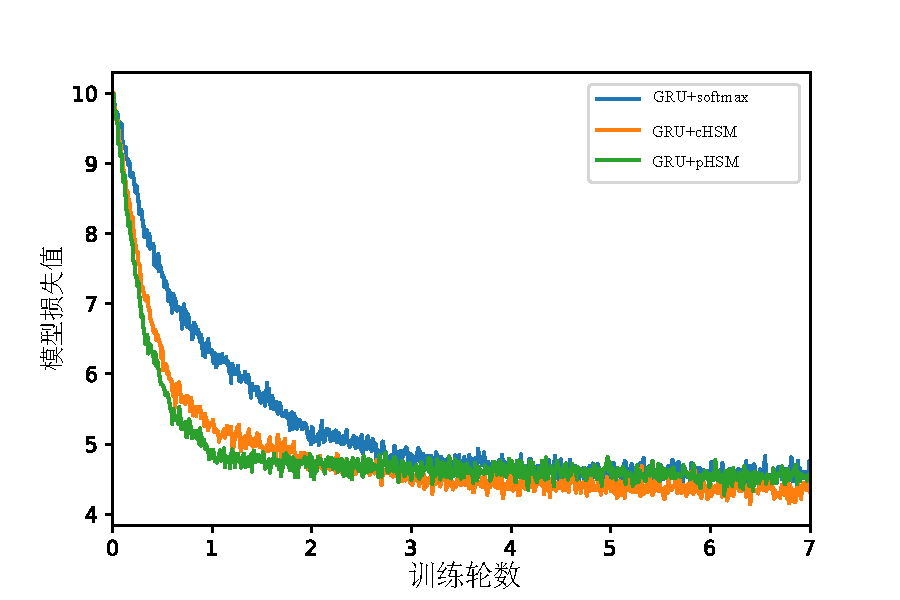
\includegraphics[width=0.6\columnwidth]{./figures/learn2.pdf}
  \caption{模型训练曲线图}
\end{figure}

另外,本实验采用~Adam~算法(Optimizer)配合两种初始学习率(Learning Rate)作为模型的优化求解函数,即设置~$\mathtt{lr}=0.06$~和~$0.001$。两种词表层次分解方法收敛速度较慢需要采用较大的学习率,而传统的softmax和采样近似方则需要采用较小的学习率。除此以外,为了减弱模型收敛过程中的损失值的振荡现象,每隔一定步数($\texttt{Step} =100$),学习率还需要逐渐缩小:$\texttt{lr}\leftarrow\texttt{lr}*0.9$。

对于在~Wikitext-2~数据集上运行的实验,设置批处理大小(Batch Size)为~20~并且最大遍历周期(Epoch)为~15。当模型在验证集上收敛后,验证集损失值大约在 4.8左右。
而~Wikitext-103~数据集设置的最大遍历周期(Epoch)大约为~5-10~个轮数,Wikitext-103~训练集大约是~Wikitext-2~的~50~倍需要的遍历周期相对更少。
当模型在验证集上收敛后,验证集损失值大约在~5.1~左右,Wikitext-103~的词表相对更大导致模型的预测困惑度更高。
实验发现~Wikitext-2~和~Wikitext-103~的唯一区别是训练数据的大小,增大训练数据集不一定能保证模型在相同的验证和测试集上结果更好,因为训练数据训练集增大~50~倍的同时词表也增大了~3~倍。

此外,在~OBW~数据集上运行的实验需要更大的参数集合来拟合导致计算缓慢同时收敛也缓慢。
为了减少计算时间,本实验应用~CuDNN~实现的~RNN~模型~\upcite{DBLP:journals/corr/AppleyardKB16},这将会把~RNN~部分所需要的计算时间降到最低,然而实际模型收敛时间也需要大约~480~小时。

\section{影响因素比较}

这部分将讨论语言模型的大词表问题在具体实验中瓶颈和各种不同优化策略对该问题的计算效率和性能的提升和分析。
\begin{figure}[!b]
  \centering
  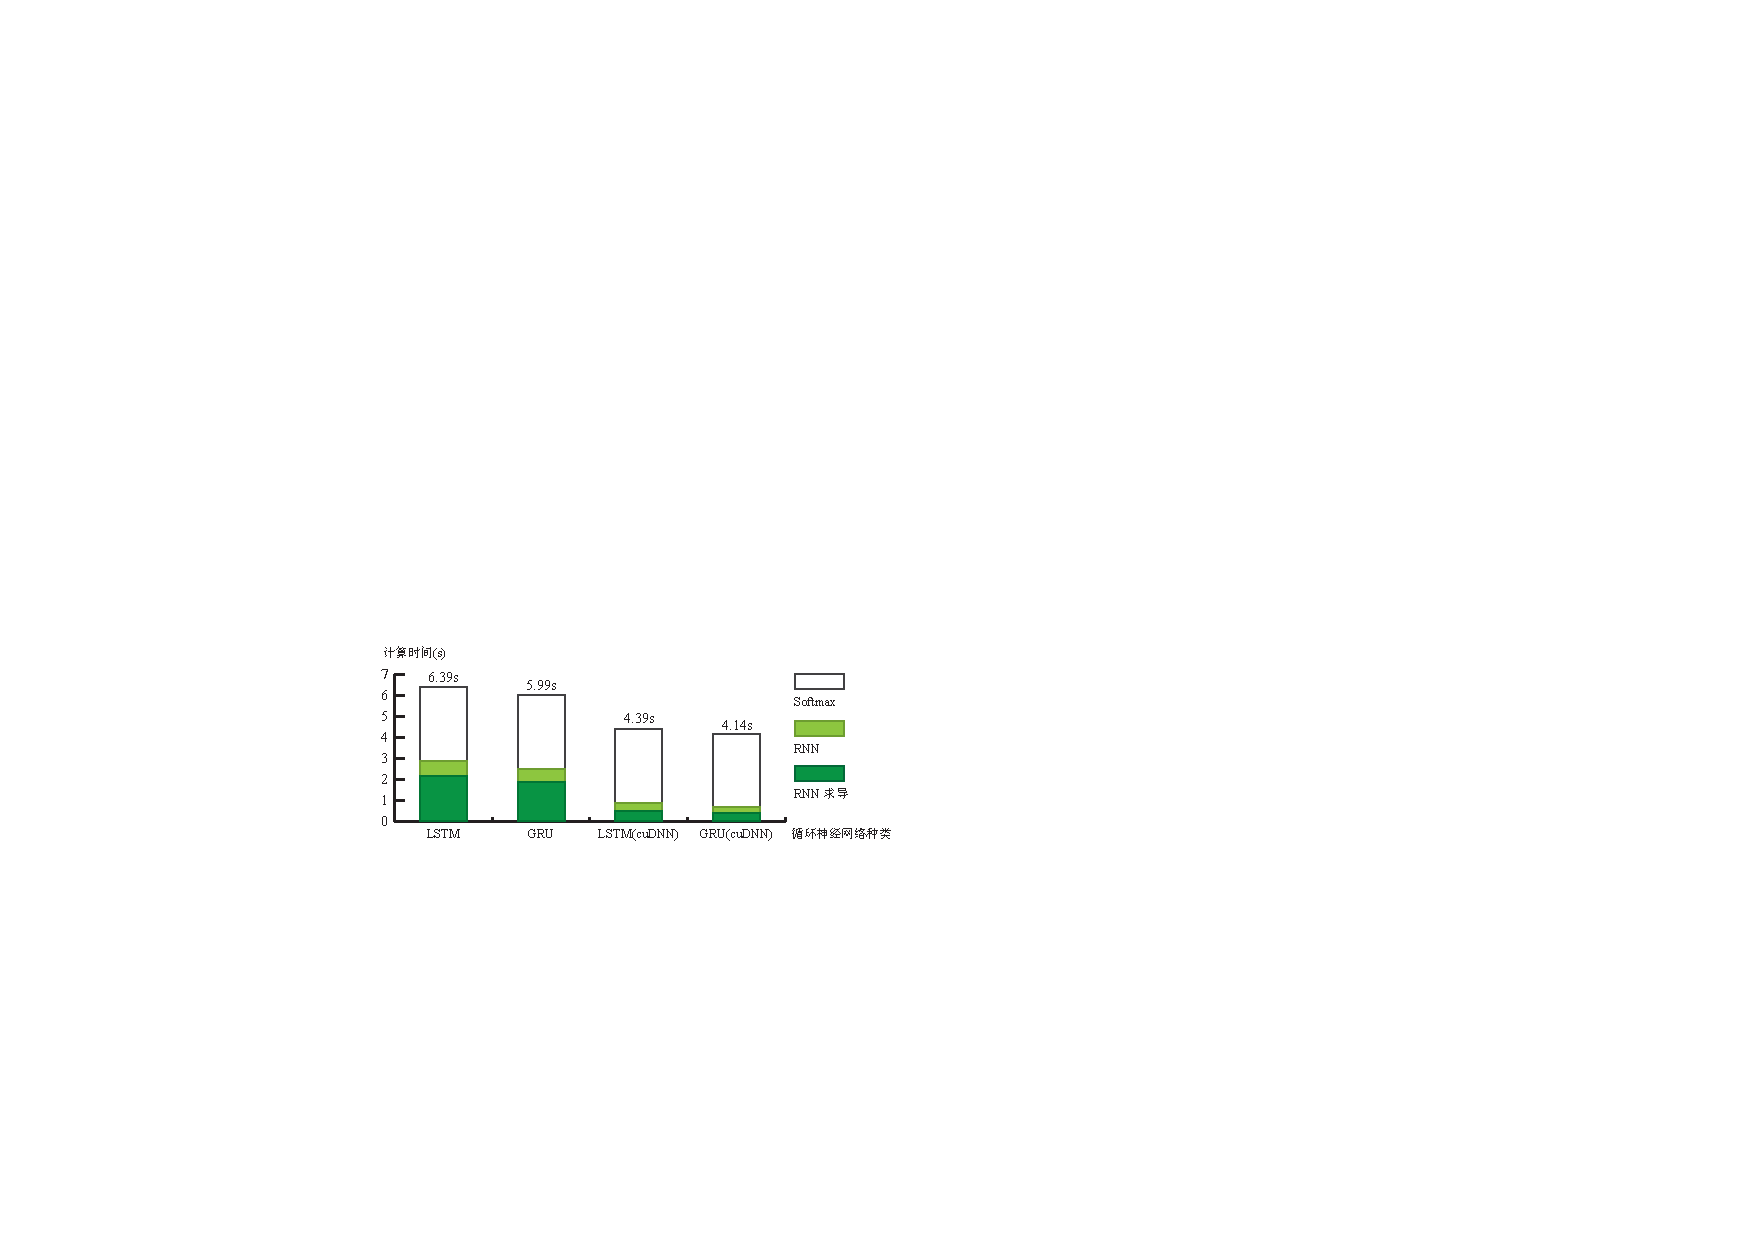
\includegraphics[width=.9\columnwidth]{./figures/rnn_timing.pdf}
  \caption{Wikitext-103数据集上测量语言模型三个部分的计算时间比较}\label{fig:rnn_timing}
\end{figure}
\subsection{大词表问题实验分析}

考虑到~Wikitext-103~数据集的词表大小与平时所采用的数据集的词表相当,本文首先在该数据集上统计了语言模型中每个模块的计算时间消耗,统计softmax函数、不同的RNN结构(即LSTM~模型和~GRU~模型)及其梯度(即,RNN Gradient)所需的时间,如图~\ref{fig:rnn_timing}~所示。
我们分别用~Theano~框架和~CuDNN~实现了~RNN~模块,前两组采用~Python~语言实现,后两组的RNN模块的核心计算部分使用~C++~语言实现,同时采用~Python~完成调用的封装函数。目前基于~CuDNN~实现的~RNN~模型计算时间最快,保证~RNN~模块的运行时间可以缩减到最短。 我们将实验重复了~100~遍并统计每个模块的平均占用的时间消耗,其目的是通过多次实验来保证实验数据准确性并减少随机误差。


从图~\ref{fig:rnn_timing}~中可以看出,使用基于~CuDNN~实现的~RNN~模块之后,softmax~模块占用的时间远超过总时间的~80\%并且~softmax~函数计算时间占比随着词表的增大而越来越大,这就需要我们详细讨论~softmax~函数的优化。


\subsection{词表层次化比较}
表~\ref{tab:time}~中统计了不同层次概率模型在~WikiText-103~数据集上的平均计算时间消耗。
其中输入句子的最大长度是$50$,隐藏层维度为$256$,输出端的词表大小是$267735$和批量处理大小设置为 20。此外,``总计算时间''表示模型的前向概率计算和后向梯度优化的过程,``前向计算时间 ''表示从输入数据到计算模型代价函数所消耗的时间,同时还给出了不同算法在训练中的内存占用。$\mathcal{|V|}$~表示词表大小,$\mathcal{|H|}$~是隐藏层维度。

由该表分析可知,在训练训练过程中tHSM算法消耗最小的内存,而p-tHSM算法需要消耗相对较大的内存。同时p-tHSM算法在三类统计项中计算速度都是最高的,只有在GPGPU配置的代价函数计算环节比cHSM算法慢。

\begin{table}[!ht]
  \centering
  \caption{Wikitext-103数据集上GPGPU和CPU的运行时内存和计算时间比较\label{tab:time}}
\begin{tabular}{lccccc}
  \toprule
 \multirow{2}{*}{算法}  &\multirow{2}{*}{运行时内存占用} &\multicolumn{2}{c}{总计算时间 (ms)} & \multicolumn{2}{c}{前向计算时间 (ms)}   \\
   \cmidrule(lr){3-4}  \cmidrule(lr){5-6}
	& & CPU&GPGPU & CPU& GPGPU \\ \midrule
Softmax & $\mathcal{|HV|}$ &510.4  &262.1&352.2& 62.9 \\
cHSM    & $2\mathcal{|H|\sqrt{|V|}}$&506.5  &\textbf{40.6}&28.7&14.6 \\
tHSM    &$\mathcal{|H|}$&1,004.0 &444.4 & 8.1&  5.6   \\
p-tHSM  &$\mathcal{|H|\log{|V|}}$ &\textbf{383.5}&	86.4 &\textbf{7.0}&	\textbf{1.4} \\
  \bottomrule
\end{tabular}
\end{table}

\begin{figure}[!t]
  \centering
  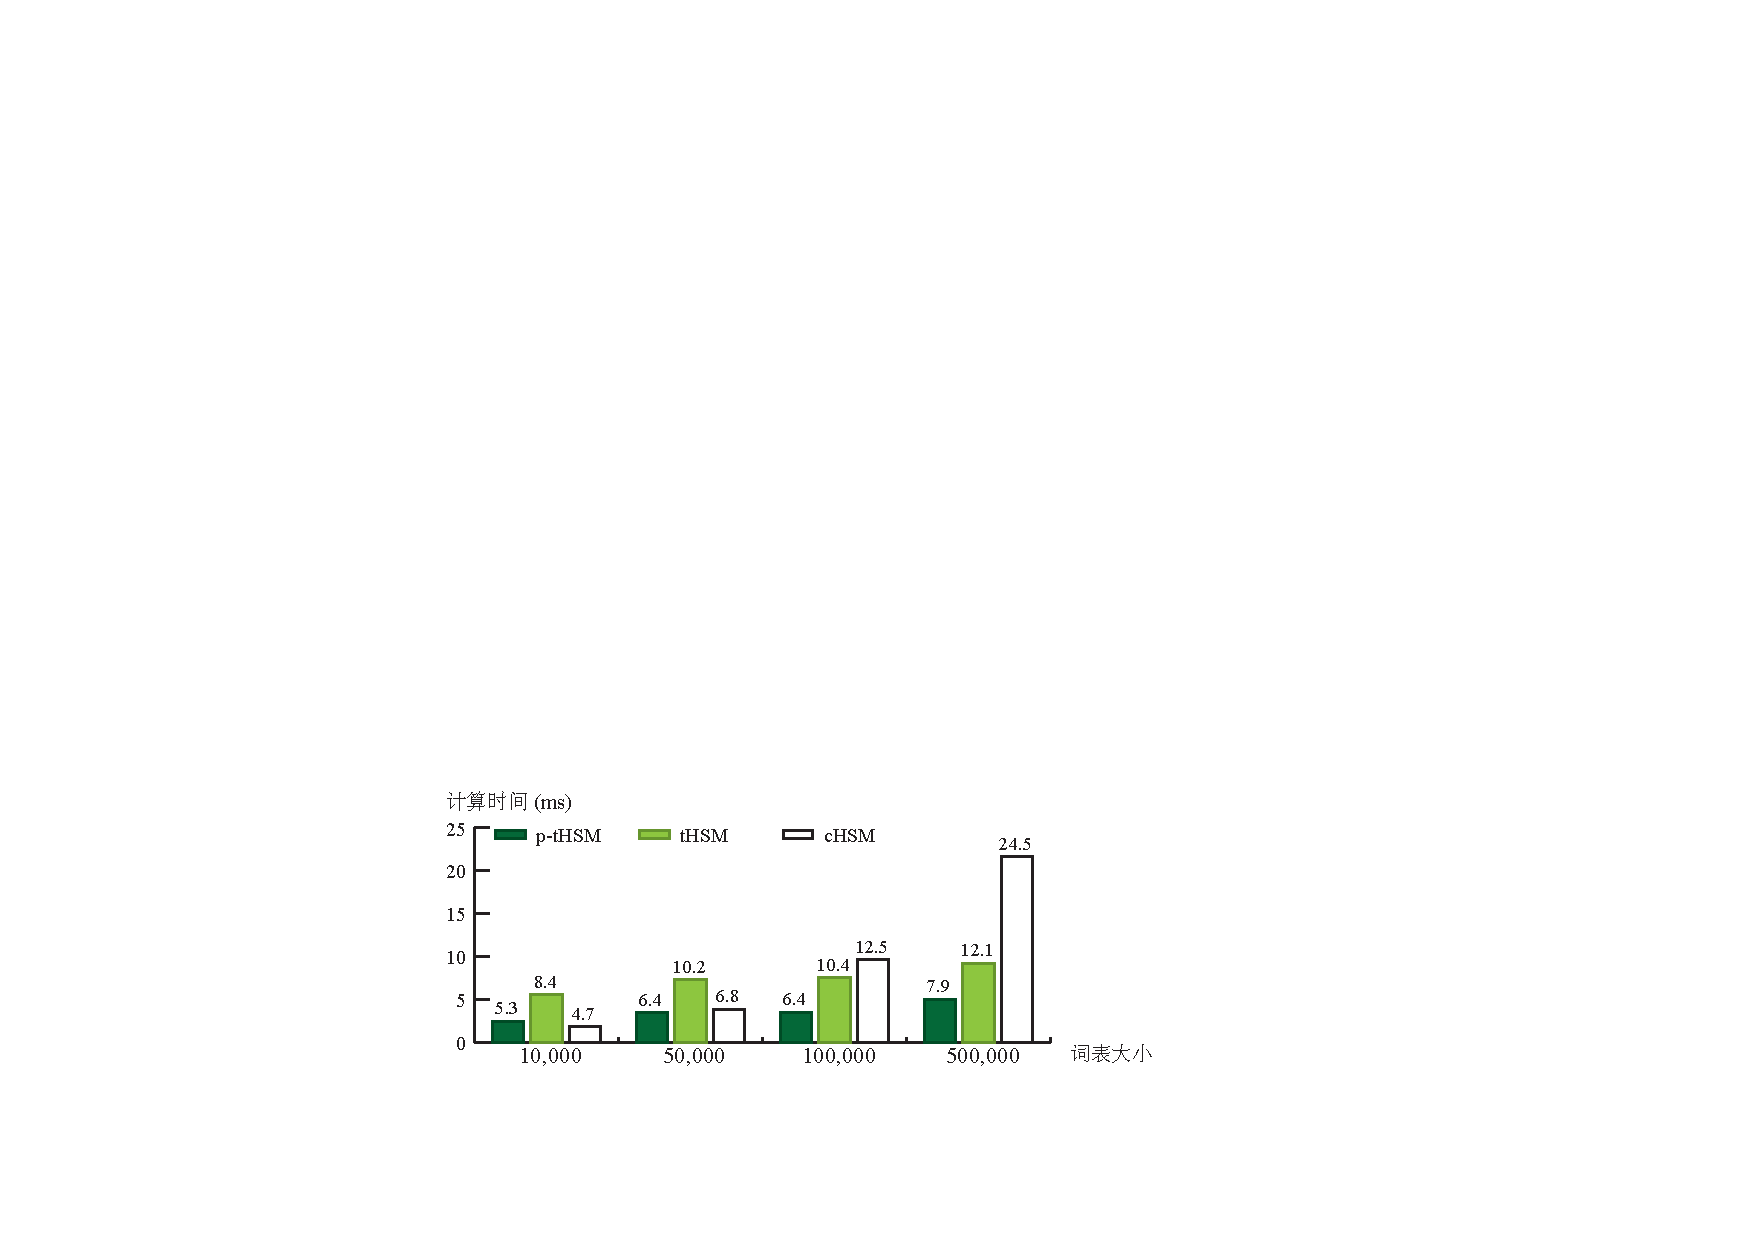
\includegraphics[width=.87\columnwidth]{./figures/all_time.pdf}
  \caption{cHSM、tHSM 和 p-tHSM 算法随着词表大小的计算时间影响}\label{fig:hsm_benchmark}
\end{figure}

\subsection{词表伸缩性比较}
图~\ref{fig:hsm_benchmark}~验证cHSM、tHSM和p-tHSM算法对词表大小的伸缩性的实验结果,这里不包``softmax''方法,因为与其他算法相比,它消耗相当多的计算时间无法被放在这个图里面。 从图中分析得知,cHSM计算时间与词表的平方根呈线性关系(即,$\mathcal{O(\sqrt{|V|})}$),tHSM算法的计算时间与词表的对数成线性关系 (即,$\mathcal{O(\log{|V|})}$)。同时本论文中提出的p-tHSM算法的计算效率相比于tHSM算法更高。这是由于是传统tHSM算法需要逐个访问树的节点对应的参数向量,花费了部分时间在矩阵的Indexing操作中,而本文提出的算法则直接将路径上所有的参数向量加载进内存直接避免了该Indexing操作,从而达到了计算效率的提升。
%在这些实验的基础上,我们可以得出结论:所提出的p-tHSM方法胜过历史记录~$\mathcal{O(|H|\log|V|)})$,并且取得了令人满意的分层softmax方法的加速比。 这种性能归因于基于GPGPU并行性的加速,也是由于p-tHSM 方法的基本结构,能够将目标字树进行并行地计算。


\subsection{搜索策略的影响}
接下来分析模型在测试过程中的不同的搜索策略对实验指标WER的影响,如表~\ref{tab:psearch}~和表~\ref{tab:csearch}~所示。


算法~\ref{alog:global}~表示先计算所有单词的得分然后再做排序。对于~p-tHSM~算法,我们比较了所提出的算法~\ref{alog:greed_argmax}~和传统的算法~\ref{alog:global}在计算速度和准确度上的实验分析。算法~\ref{alog:greed_argmax}~比算法~\ref{alog:global}~方法计算结果花费的时间更少。由于基于树的模型在逐层访问路径的过程中更容易出现错误情况,所以算法~\ref{alog:global}~的WER分数比算法~\ref{alog:greed_argmax}~相对更好。
\begin{table}[!ht]
  \centering
  \caption{Wikitext-2数据集上~p-tHSM~算法针对不同搜索算法的WER评测结果\label{tab:psearch}}
\begin{tabular}{ccccc}
  \toprule
     层次概率模型   & 算法类别&计算时间(ms)&验证集(WER)& 测试集(WER)\\ \midrule
  \multirow{2}{*}{p-tHSM}  &全局计算(算法~\ref{alog:global})&161& \textbf{76.67\%}&\textbf{75.35\%}\\
        &贪心计算(算法~\ref{alog:greed_argmax})&\textbf{30} & 79.61\%&79.32\%\\
  \bottomrule
\end{tabular}
\end{table}

\begin{table}[!ht]
  \centering
  \caption{Wikitext-2数据集上~cHSM~算法针对不同搜索算法的~WER~评测结果\label{tab:csearch}}
\begin{tabular}{ccccc}
  \toprule
  层次概率模型 & 算法类别&计算时间 (ms)&验证集(WER)& 测试集(WER)\\ \midrule
  \multirow{3}{*}{cHSM} &全局argmax(算法~\ref{algo:alls})&102& 80.00\%& 80.02\%\\
        &贪心argmax(算法~\ref{alog:exact})&87& 80.00\%& 80.02\%\\
        &伪贪心argmax(算法~\ref{alog:cargmax})&\textbf{44}& 82.09\%&  82.07\%\\
  \bottomrule
\end{tabular}
\end{table}


算法~\ref{alog:exact}~比算法~\ref{algo:alls}~WER指标相同,但是算法~\ref{alog:exact}~计算速度相对较快,这是因为算法\ref{alog:exact}避免了不断调用$p^c$的概率的冗余操作。同时算法~\ref{alog:cargmax}~的计算速度相比于其他更快,但是损失了模型的预测精度。


\subsection{门限机制的影响}

如表~\ref{tab:rnn}~所示,在 PPL,WER 这两种指标评测中,拥有门控单元的~LSTM~和~GRU~网络比传统的~RNN Relu~和~RNN Tanh~模型表现得更好,这是因为门控单元可以避免循环网络中的梯度消失的问题。在计算时间的评测指标上,传统的网络结构比带有门限机制的网络计算效率更高,同时从表中分析发现~LSTM~比~GRU~模型需要更少的计算时间。这是由于~LSTM~的计算公式中参数的相似性和独立性,我们可以并行计算各个门节点,然而~GRU~模型之间计算步骤存在较大的依赖关系,需要按时序计算,进而LSTM计算速度稍快于GRU模型。

\begin{table}[!ht]
  \centering
  \caption{Wikitext-2数据集上不同循环网络针对 PPL、 WER和计算时间的影响\label{tab:rnn}}
\begin{tabular}{lccc}
  \toprule
  循环神经网络 & 计算时间(ms)&验证集(PPL / WER) & 测试集(PPL / WER)\\ \midrule
  1$\times$RNN Relu~\cite{DBLP:journals/jmlr/GutmannH10} &176.4&260.52 / 80.00\%&238.75 / 80.02\%\\
  1$\times$RNN Tanh~\cite{DBLP:journals/iclr/JiVSAD15}   &176.2&250.57 / 79.61\%&230.98 / 79.32\%\\
  1$\times$LSTM~\cite{7508408}                  &\textbf{189.5}&180.98 / 77.16\%&165.60 / 76.67\%\\
  1$\times$GRU~\cite{DBLP:journals/corr/ChungGCB14}      &191.3&\textbf{179.59 / 77.09\%}&\textbf{165.32 / 77.07\%}\\ \midrule
  2$\times$RNN Relu~\cite{DBLP:journals/jmlr/GutmannH10} &266.3&190.52 / 73.01\%&198.75 / 73.02\%\\
  2$\times$RNN Tanh~\cite{DBLP:journals/iclr/JiVSAD15}   &266.3&189.57 / 72.62\%&260.98 / 72.32\%\\
  2$\times$LSTM~\cite{7508408}                  &\textbf{279.4}&164.98 / 71.17\%&165.60 / 71.67\%\\
  2$\times$GRU~\cite{DBLP:journals/corr/ChungGCB14}      &281.2&\textbf{158.59 / 70.08\%}&\textbf{155.32 / 70.07\%}\\
  \bottomrule
\end{tabular}
\end{table}

\subsection{截断~BPTT~的影响}
接下来分析RNN模型的反向求导模块对实验结果的影响。在~RNN~模型求导数过程中,因为隐藏层是随时间共享的,所以计算导数的时候求导链需要反向传播(Back Propagation Through Time,BPTT)。若是批量数据输入,模型的求导链的计算代价与该批次文本中最长的序列长度相同。考虑到不同批次中的句子长度各异,该求导算法可以通过截断求导链的方式减少模型计算量,该方法被称为截断~BPTT~算法。其优点是模型的各个步骤的损失值计算反向导数的步数是一致的,与句子的长度无关,进而模型的训练速度有所提升。如图~\ref{fig:minibatch}~所示,前向概率计算步骤仍然是相同的,唯一的影响是避免过长的梯度反向传播步骤。


\begin{figure}[!t]
  \centering
  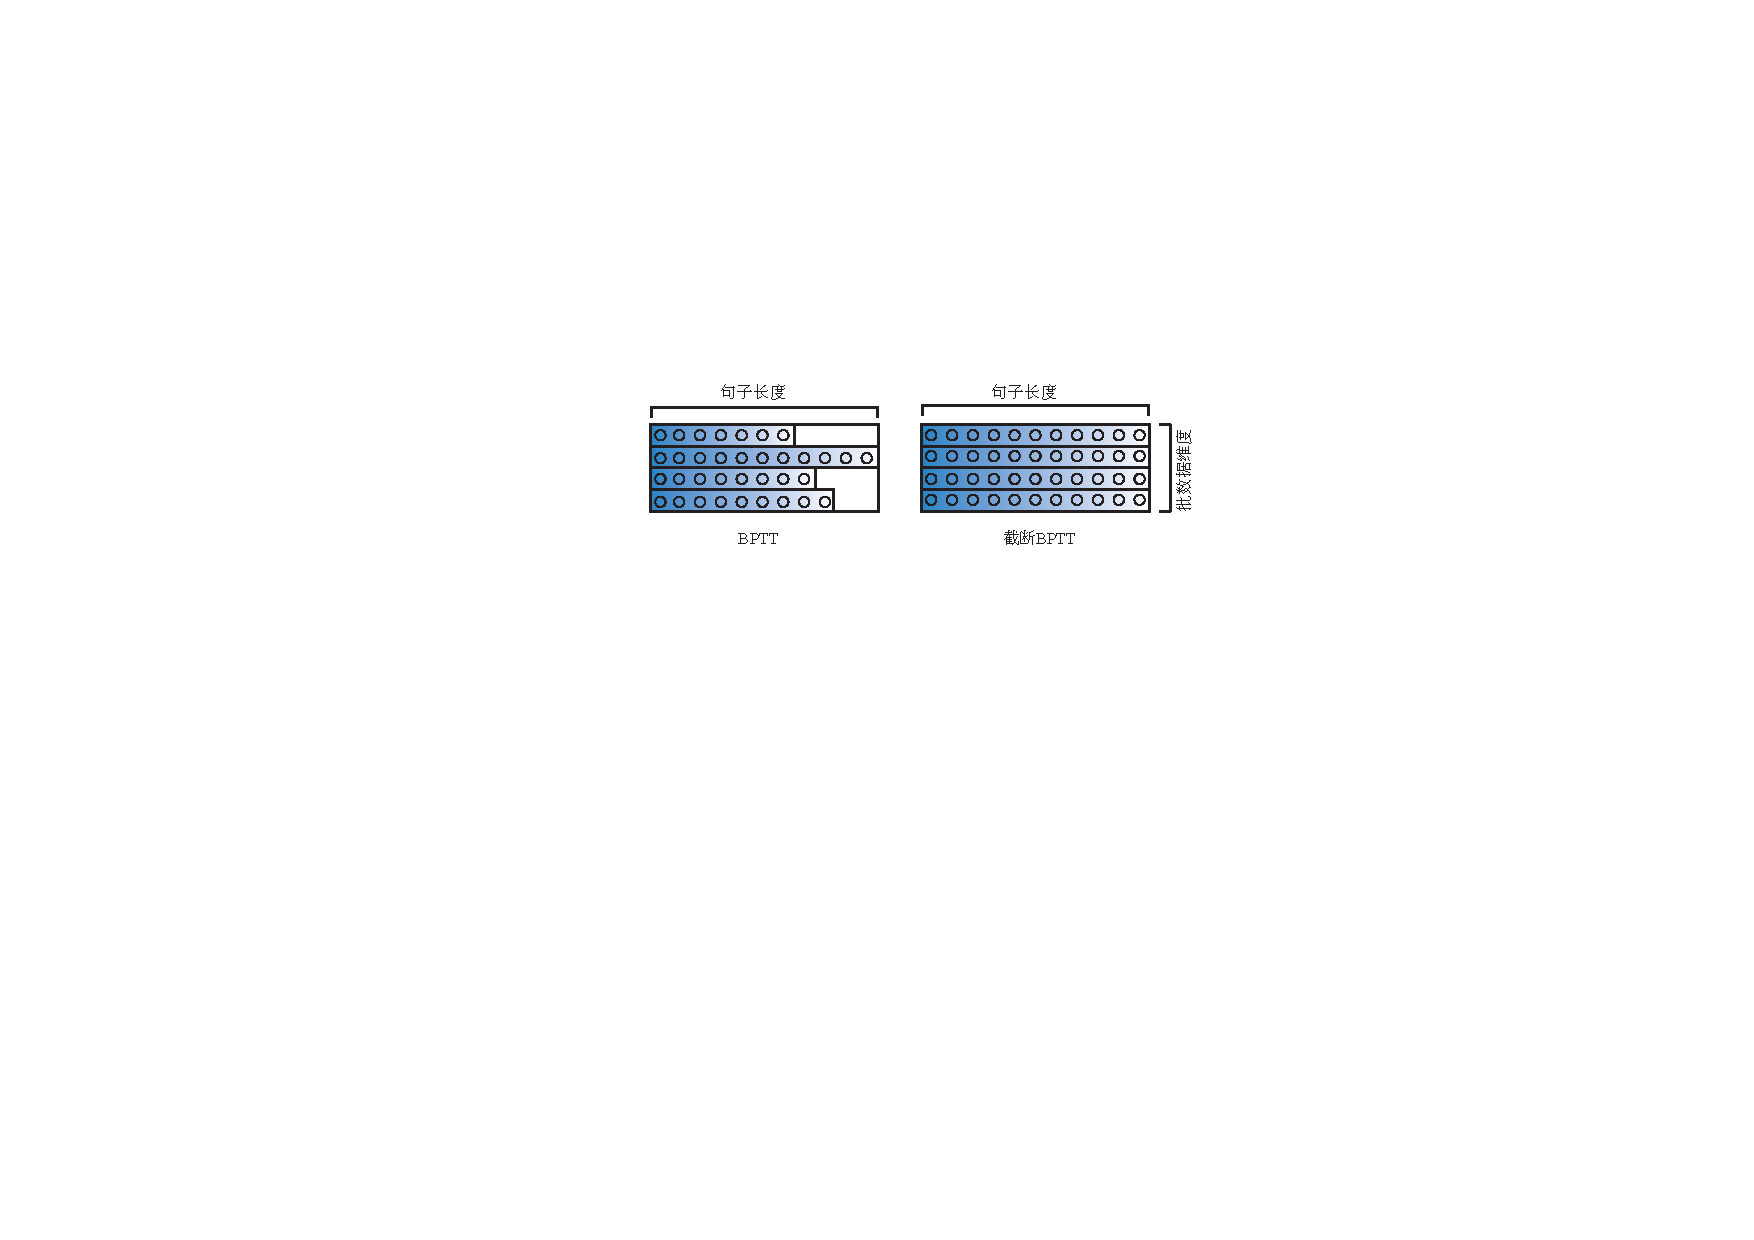
\includegraphics[width=.75\columnwidth]{./figures/minibatch.pdf}
  \caption{BPTT和截断BPTT算法示意图}\label{fig:minibatch}
\end{figure}

其次说明截断~BPTT~操作与文本的长距离依赖之间的关系。在训练过程中,如果依赖关系存在于被截断的语句中,则模型可以学习这种关系; 如果依赖关系总是跨越不同的语句块,那么被截断的语句中不存在这种该依赖关系,从而模型将无法学习这种关系。 其原因是模型的参数导数无法回溯到最初的跨段的那个单词,进而无法更新相应的参数学习这种跨段的依赖关系。
如果这种依赖关系仅存在于单个语句段中,由于模型的参数能求导到前面对应的单词,模型能学习到这种关系。
然而在测试时,模型不存在这个限制,它能在跨语句段中预测这种依赖关系, 因为模型的计算步骤是不断向前传播,不存在模型反向求导的计算过程。
\begin{figure}[!ht]
  \centering
  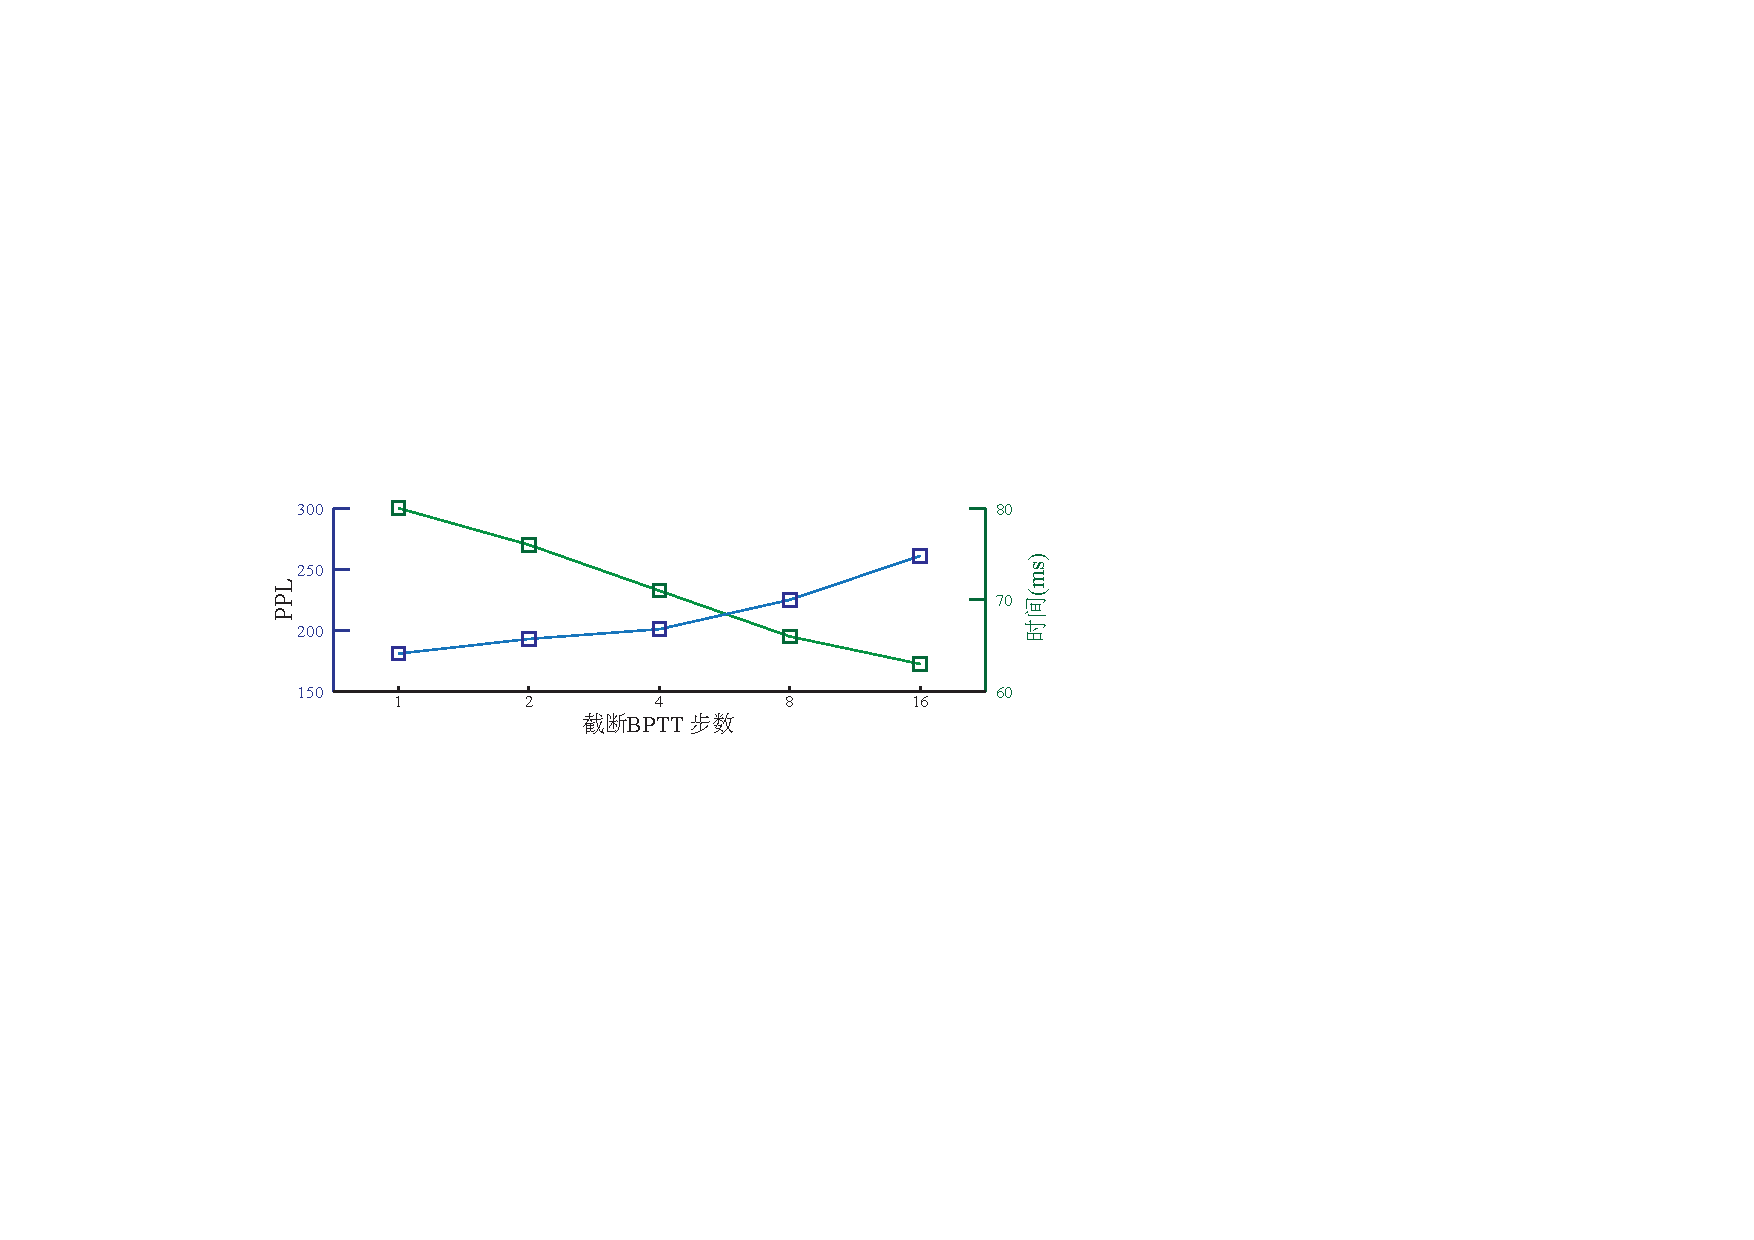
\includegraphics[width=.85\columnwidth]{./figures/tbptt.pdf}
  \caption{Wikitext-2数据集上 BPTT和截断BPTT算法对RNN的影响}\label{fig:tbptt}
\end{figure}

从图~\ref{fig:tbptt}~中可以看出,截断BPTT较小时模型的时间计算速度相对较高同时模型的的PPL数值较高,截断BPTT较大时模型的时间计算速度相对更慢同时模型的的PPL数值较低。


\subsection{采样近似算法比较}
基于采样估计的算法的效率和准确性与样本大小密切相关,从而这小节将评测了两种采样算法的性能。
本实验测试不同采样样本数~$k$~对模型的训练和测试的结果的影响,结果展示在图~\ref{fig:blackout_nce}中。
从图中分析,在平均每次迭代中~Blackout~算法收敛性比传统的~NCE~算法相对更好,但是~NCE~算法计算效率比~Balckout~更高。所以在单位时间中~NCE~算法收敛速度更快,这与~Ji~等人的实验结果是一致的~\upcite{DBLP:journals/iclr/JiVSAD15}。同时在该实验中,当$k=1$时,采样函数计算的就是真正的二元分类概率,此时采样算法振荡现象很剧烈,无法收敛。当逐渐增大采样样本数~$k$,采样算法才能逐渐开始收敛。两种算法的加速比均是~$V/k$,与超参数~$k$~呈负相关关系。

\begin{figure}[!t]
  \centering
  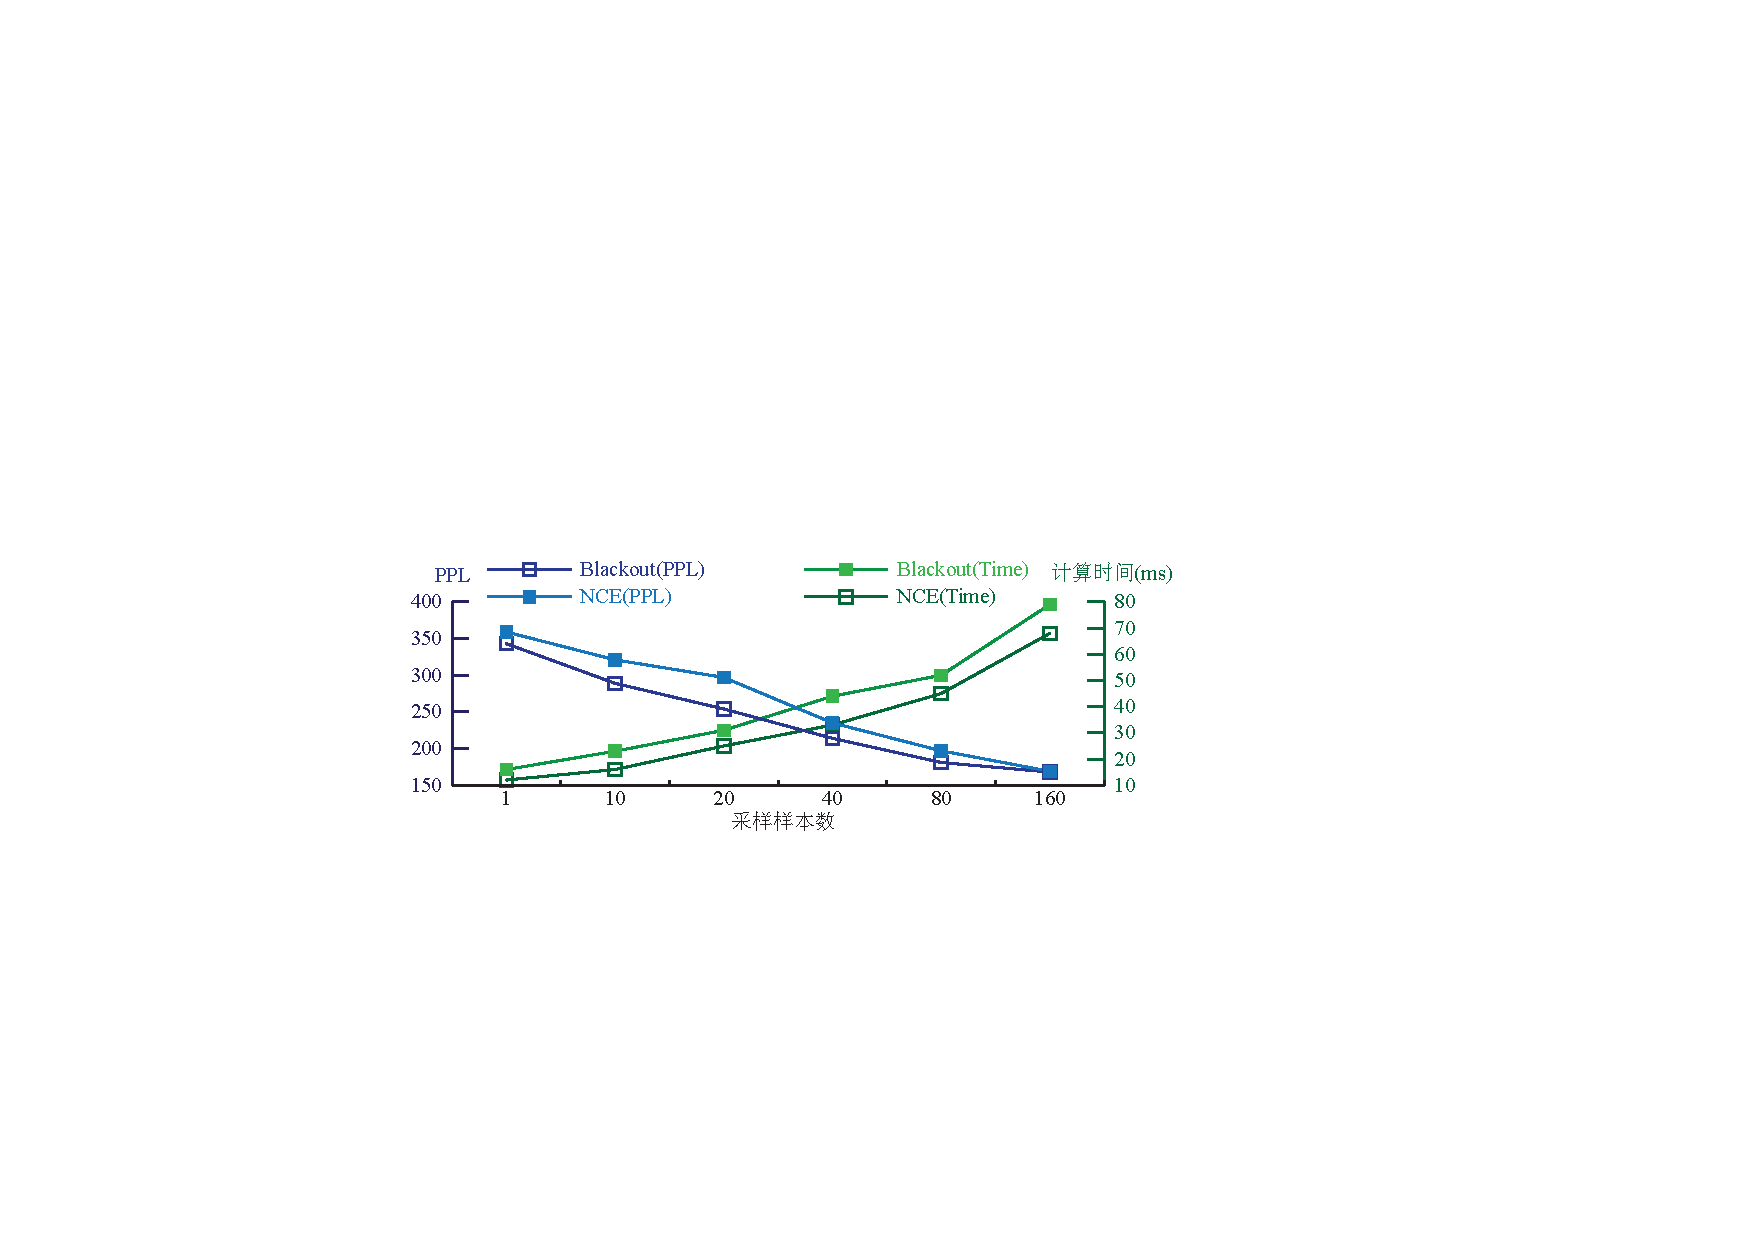
\includegraphics[width=.85\columnwidth]{./figures/nce_blackout.pdf}
  \caption{Wikitext-2上测试不同采样数量对NCE和Blackout算法的影响}\label{fig:blackout_nce}
\end{figure}


\subsection{单词聚类策略分析}
Chen~等人发现~cHSM~和~p-tHSM~算法的性能对不同单词的层次聚类算法很敏感~\upcite{DBLP:conf/acl/ChenGA16},因此为了获得较为稳定的~cHSM~算法和~p-tHSM~方法,本文考虑已有的聚类策略,结果展示在表~\ref{table:p-thsm}~和表~\ref{table:clustering}~中。

\begin{table}[!ht]
  \centering
   \caption{Wikitext-2上评价不同聚类方法对p-tHSM 算法的PPL影响\label{table:p-thsm}}
  \begin{tabular}{lcccc} \toprule
  算法  &建树时间&最大树深度 &验证集 (PPL) & 测试集 (PPL)  \\ \midrule
  Uni-gram  &3分钟&12 &218.42& 216.05     \\
  Bi-gram  &35小时&21& 186.23& 189.58\\
  Semantic &26小时 &18& \textbf{163.12} & \textbf{178.78}\\
\bottomrule
  \end{tabular}
\end{table}

对于基于树的层次算法的初始化,我们采用了霍夫曼聚类、布朗聚类和词向量聚类三种方法来生成不同的单词分布,详细的结果展示在表~\ref{table:p-thsm}~中。与能调整分支因子数目的~cHSM~方法不同,p-tHSM~算法由于子树最后都合并到根节点,所以不需要调整分支因子数。从实验结果中分析得知,一方面Uni-gram~聚类方法在创建单词层次结构方面效率最高,而~Bi-gram~和语义聚类需要花费巨额时间来计算词表中单词之间的相似度矩阵。另一方面,针对聚类的距离尺度,Uni-gram~以单词的词频为权重,Bi-gram~方法考虑二元共现单词的统计信息,语义聚类方法则计算特征空间中的两单词的余弦距离。在~PPL~指标比较中,采用~Bi-gram~和语义聚类的方法比采用霍夫曼聚类的方法拥有更低的分数。

\begin{table*}[!t]
\small
  \centering
  \caption{Wikitext-2数据集上不同聚类算法对cHSM 算法的PPL 和 WER 影响\label{table:clustering}}
  \begin{tabular}{lclccc} \toprule
聚类算法 & 均匀划分?&分支数& 训练轮数& 测试集 (PPL / WER)&耗时 (ms)\\ \midrule
  \multirow{6}{*}{Random}  &\multirow{6}{*}{是}&10/3330&145&211.15 / 78.55 &791\\
    &&20/1664&123&228.72 / 78.89&565\\
    &&40/832&103&234.36 / 79.21&321\\
    &&80/417&78&243.12 / 79.64&171\\
    &&160/208 &57&253.38 / 80.08&92\\
    &&182/183&48&268.63 / 80.11&88\\
  \midrule
  \multirow{6}{*}{Alphabet}  &\multirow{6}{*}{是}&10/3330 &141&199.01 / 78.07 &773\\
    &&20/1664 &120&211.34 / 78.23&551\\
    &&40/832 &100&238.75 / 79.02&313\\
    &&80/417 &90&241.75 / 79.34&174\\
    &&160/208 &56&248.35 / 79.62&97\\
    &&182/183&45&258.57 / 80.02&87\\
  \midrule
  \multirow{6}{*}{Uni-gram}   &\multirow{6}{*}{是} &10/3330&134&211.51 / 77.41 &788\\
    & &20/1664&122&220.01 / 77.71&549\\
    & &40/832&113&236.56 / 77.95&302\\
    & &80/417&91& 241.12 / 78.25&170\\
    & &160/208&55&247.25 / 79.21&93\\
    & &182/183&42&253.35 / 79.92&86\\
  \midrule
  \multirow{5}{*}{Bi-gram}   &\multirow{5}{*}{否}&10/3672&150&208.11 / 77.32&801\\
     &&20/1923&121&217,34 / 77.64&621\\
     &&40/1123&102&228.87 / 78.14&588\\
     &&80/572&89&246.32 / 78.43&186\\
     &&160/340&76&252.33 / 79.51&97\\
  \midrule
  \multirow{5}{*}{Syntactic}  &\multirow{5}{*}{否}&10/3612 &152&214.31 / 78.11&810\\
    &&20/1972 &130&220.19 / 78.86&633\\
    &&40/996 &101&232.33 / 79.33&543\\
    &&80/545 &89&241.34 / 79.84&179\\
    &&160/235 &70&262.34 / 80.14&134\\
  \midrule
  \multirow{5}{*}{Semantic}  &\multirow{5}{*}{否} &10/3570 &133&208.77 / 77.41&819\\
    & &20/1873 &114&218.31 / 77.78&641\\
    & &40/1092 &91&225.38 / 78.35&521\\
    & &80/561 &69&238.45 / 78.91&174\\
    & &160/244 &44&256.75 / 79.41&103\\
\bottomrule
  \end{tabular}
\end{table*}

表~\ref{table:clustering}~讨论了在~Wikitext-2~数据集上,cHSM~算法上应用前章节所介绍的不同聚类方法之间的差异,同时比较了不同的分支因子对算法效果的影响。从该表的结果分析得出,随机初始化方法性能最差,因为它没有提供有效的先验信息,从而干扰模型的学习过程。
此外还观察到,随机初始化的策略具有更大的训练误差需要更多的训练轮数来使之收敛。
然后,发现在对模型的类结构注入Uni-gram和Bi-gram的信息之后,模型能在特征空间学习到相对较好的单词分布。
因此,这两者比随机初始哈和按字母顺序初始化的算法在PPL和WER两种指标上结果更好。

而且,用语法和语义聚类算法将词表进行切分,能比其他的分割算法取得更好的PPL和WER数值。这间接表明,若能将有效的正确的知识注入模型的训练过程,模型理论上将获得更好的概率分布和更优良的稳定性。相比于二叉树层次概率模型,该算法还能动态调整分支因子,模型的适用范围相对更广。

\section{模型总体评价}
表~\ref{tab:summary_ppl}~统计了所有模型在上述三种标准语料的验证和测试数据集的PPL和WER结果。我们采用单层GRU单元作为这些算法的上下文表示,其维数设置为256。另外,对于~NCE~和~Blackout~采样算法,超参数~$k$~对较小的~Wikitext-2~和~Wikitext-103~数据集设置为$\mathcal{|V|}/20$,对于较大的~OBW~数据集设置为~$k=|\mathcal{V}|/200$。 此外,对于~cHSM~方法,我们根据单词的词频分布来划分词表。

\begin{table}[!t]
  \centering
  \caption{所有模型在三个数据集上的PPL和WER的性能评测\label{tab:summary_ppl}}
\begin{tabular}{llcc}
  \toprule
数据集& 算法& 验证集(PPL/WER) & 测试集(PPL/WER) \\ \midrule
 \multirow{2}{*}{WikiText-2}&GRU + Softmax&172.64 / 77.49\%&162.09 / 77.07\% \\
  &GRU + NCE~\cite{DBLP:journals/jmlr/GutmannH10}&217.84 / 78.26\%&199.54 / 78.02\%\\
  &GRU + Blackout~\cite{DBLP:journals/iclr/JiVSAD15}&221.15 / 77.72\%&199.56 / 77.50\% \\
  &GRU + cHSM + Uni-gram~\cite{DBLP:conf/acl/ChenGA16}&203.18 / 78.25\%&206.61 / 78.02\%\\
  &GRU + p-tHSM + Uni-gram~\cite{DBLP:conf/nips/MikolovSCCD13}&218.42 / 78.15\%&216.05 / 78.15\%\\
  &GRU + p-tHSM + Bi-gram~\cite{DBLP:journals/coling/BrownPdLM92}&186.23 / 78.15\%&189.58 / 78.15\%\\\midrule
   \multirow{2}{*}{WikiText-103} &GRU + Softmax&130.38 / 72.15\%&136.83 / 72.37\%\\
 &GRU + NCE~\cite{DBLP:journals/jmlr/GutmannH10}&164.78 / 73.22\%&165.01 / 73.34\%\\
  &GRU + Blackout~\cite{DBLP:journals/iclr/JiVSAD15}&163.99 / 73.18\%&162.76 / 74.22\%\\
  &GRU + cHSM + Uni-gram~\cite{DBLP:conf/acl/ChenGA16}&161.81 / 73.42\%&156.74 / 73.18\%\\
  &GRU + p-tHSM + Uni-gram~\cite{DBLP:conf/nips/MikolovSCCD13}&165.70 / 73.53\%&166.11 / 72.44\%\\
  &GRU + p-tHSM + Bi-gram~\cite{DBLP:journals/coling/BrownPdLM92}&164.15 / 78.15\%&163.55 / 77.85\%\\\midrule
  \multirow{2}{*}{One Billion Words} &GRU + Softmax&330.38 / 88.15\%&330.83 / 88.37\%\\
 & GRU + NCE~\cite{DBLP:journals/jmlr/GutmannH10}&272.07 / 84.83\%&276.11 / 84.34\%\\
  &GRU + Blackout~\cite{DBLP:journals/iclr/JiVSAD15}&268.67 / 84.23\%&266.11 / 84.18\%\\
 & GRU + cHSM + Uni-gram~\cite{DBLP:conf/acl/ChenGA16}&225.36 / 80.32\%&224.11 / 79.42\%\\
 & GRU + p-tHSM + Uni-gram~\cite{DBLP:conf/nips/MikolovSCCD13}&231.44 / 87.53\%&236.11 / 82.53\%\\
  %&GRU + p-tHSM + Bi-gram~\upcite{DBLP:journals/coling/BrownPdLM92}& 221.55 / 81.15\%&218.70 / 83.15\%\\
  \bottomrule
\end{tabular}
\end{table}

对于~Wikitext-2~数据集上的结果分析发现,softmax比其他算法的准确度更好,这是因为引入采样函数或者层次结构将会一定程度上加入人为的先验分布同时丢失了一部分信息,这妨碍了模型的训练收敛过程。

对于第二个Wikitext-103数据集,基于布朗聚类的p-tHSM方法获得了比霍夫曼聚类方法更好的PPL值和WER结果,另外布朗聚类用于初始化cHSM模型也能获得很好的准确率结果。由于Wikitext-103和Wikitext-2数据集共享相同的测试集,因此发现模型在大数据集上可以收敛到更好的结果 ,这证明了添加训练数据是一种提高模型的精度的有效途径。此外,对于采样算法的收敛结果比softmax方法好得多,同时提高了时间效率。
\section{本章小结}
本章首先定量分析了大词表问题,接下来比较了本文提出的层次概率模型的计算效率和传统算法之间的差异。针对层次模型的初始化算法,我们讨论并评估三种不同的层次聚类算法,以更有效的方式组织结构化的词表。结果表明,与其他概率归一化方法相比,本文提出的层次概率算法具有很好的计算速度提升效果。同时还讨论了两种层次概率模型的适用范围和两者的优缺点。
%在未来的研究中,我们计划探索softplus函数的应用场景,并探讨在cHSM算法训练的时候的词表动态交换算法。另外,实验中应用的几种聚类算法消耗了很多时间,我们可以优化该聚类算法,设计更高效的分层结构。

%\summary
大词表问题是语言模型应用中最重要的挑战之一,为了解决这个问题,文献中提出了各种方法可大致分为三个类别:词汇截断算法,基于抽样的近似算法和词表层次分解。第三种方法将目标词汇的扁平化架构改变为具有两种可能的分层结构:类和树层次分解。构建在两步softmax分类方法和树模型上的类方法将其扩展到$\mathcal {O(| H | \log | V |)} $步骤的二进制分类。Mikolov~曾提出使用基于二叉树的层级概率模型来加速的训练方案,加速比能达到理论的最大速度,但是当时提出的背景是基于CPU构建的,如今越来越多的算法随着应用领域的推广,需要在并行度更高的~GPGPU~设备上进行计算,因此基于GPGPU进行建模的层次概率模型尚未被研究提及,需要在本文中研讨。
\section*{工作总结}
多层分类模型需要将单词按照模型的架构进行划分。其中以下策略适用于~cHSM~模型:基于词频划分类别、 基于布朗聚类进行划分、按照词向量信息进行聚类等方法,另外词表是否能均划分与具体层次聚类算法相关。


\noindent 1. 本论文中,针对两种层次概率模型,首先定义了对应编码方式,同时给出了模型所涉及的参数的详细含义。接下来,我们逐步推导模型的单个节点的概率公式,单个词的概率公式和模型的代价函数。另一方面,我们将提出的~p-tHSM~算法和传统的线性~tHSM~算法进行的比较。通过比较两者计算的差异性证明我们提出的算法更适合在GPGPU等高并行设备上运算。本文还进一步讨论了模型在测试的时候所需的推理算法,因为基于层次结构的概率计算方案和传统的softmax计算方案不同,不能直接输出单个词的概率或者计算最佳的候选单词,所以我们分别针对这两个任务提出推理算法。最后,由于单词在二叉树上的分布需要初始化,我们讨论了现存的各种聚类算法效果。

\noindent 2. 在实际实验中,我们提出的层次概率模型的计算速度比传统模型相对较快。配合不同的层次聚类算法,层次概率模型也能获得较好的预测准确度和稳定性。相比于采样算法,模型能在测试的阶段也获得同样的计算加速效果。相比于传统的softmax函数,尽管层次概率模型的精确度稍低,但是模型的计算速度极大提升。

\section*{工作展望}
本文提出的层次概率模型在语言模型的各项评测上取得了有效的结果,验证了本方法的合理性。但是该方法还存在进一步提升的空间:

\noindent 1. 大规模实验数据分析验证算法:由于在现有实验环境条件下,在大数据集上的实验验证过程收敛很慢,所以目前的实验主要还是在小规模数据集上进行了初步验证,下一步将进一步在大数据集上进行验证并比较算法的差异,进一步验证算法的广泛适用性。

\noindent 2. 由于我们选择的建模平台是python语言,优点是可以使用许多现成的已有的框架,并且python语法简单,矩阵计算库numpy和scipy更成熟,便于调试。另一方面,我们采用的建模语言是theano框架,它的底层计算都是调用BLAS计算库,或者直接调用基于CUDA的CuBLAS计算库实现的。虽然这样做便于在前期模型建立阶段能方便尝试各种设计方案,但是计算瓶颈在于python的解释器执行代码缓慢,所以如果能将部分模型组件使用CUDA语言重写,允许本论文提出的模型调试各种组合的神经网络结构,使得整体计算速度能得到更大提升,这也是许多目前流行框架发展的方向,例如Mxnet\footnote{http://mxnet.incubator.apache.org/}和caffe2\footnote{https://caffe2.ai/}直接使用~C++~语言建立深度模型,其计算效率也是目前已知的框架中最快的。因此考虑到目前的Thenao计算瓶颈,下一步将重点研究如何将RNN的框架使用CUDA语言重构,并基于CuDNN 库开发的样例代码进行改进。


\noindent 3. 本实验中采用了不同聚类算法,并分析了各个聚类算法的优劣。目前采用的聚类算法计算非常费时,尤其是当我们希望进行多层次聚类的时候,需要花费数周时间来获得结果。这样的缓慢的计算效果是无法接受的,经过针对代码的调试发现计算瓶颈在算法初始化的过程中,它花费了90\%的计算时间在计算两两单词之间的距离。如果能存在有效的初始化算法,而不是挑选尽可能高精度的聚类模型,那么实验进度和试验结果就可以针对多组参数调试。我们也可以考虑,单词分布也是随机初始化,在模型训练的时候动态计算单词交换策略,随着模型的收敛,单词的划分结构也逐渐收敛,这样一来就不需要在使用额外的计算库,给模型添加各种初始化词表分布。除此之外,还需要探讨除了语言模型的应用场景,我们还可以应用到大规模标签分类,或者更接近的机器翻译领域中。


% 参考文献
\cleardoublepage
\phantomsection
\addcontentsline{toc}{chapter}{参考文献}
\nocite{*}
\bibliographystyle{GBT7714-2005}%ZJUthesis}
\bibliography{thesis_reference}
\cleardoublepage

% 附录
%\appendix

% 附页标题样式
\backmatter
%% 附页\emph{}
\chapter{攻读硕士学位期间取得的学术成果}
% 此处标题及内容请自行更改
\noindent 发表论文:
\begin{enumerate}[label=\arabic*.]
\item \textbf{Nan Jiang}, Wenge Rong, Min Gao, Yikang Shen and Zhang Xiong. Exploration of Treebased Hierarchical Softmax for Recurrent Language Models[A]. Proceedings of the 26th International Joint Conference on Artificial Intelligence[C]. 2017: 1951-1957.
\item \textbf{Nan Jiang}, Wenge Rong, Yifan Nie, Yikang Shen and Zhang Xiong. Event Trigger Identification with Noise Contrastive Estimation[J]. IEEE/ACM Transactions on Computational Biology and Bioinformatics, 2017. (Accepted)
\item \textbf{Nan Jiang}, Wenge Rong, Baolin Peng, Yifan Nie and Zhang Xiong. Modeling Joint Representation with Tri-Modal DBNs for Query and Question Matching[J]. IEICE Transactions on Information and Systems, 2016, 99(4): 927-935.
\item \textbf{Nan Jiang}, Wenge Rong, Baolin Peng, Yifan Nie and Zhang Xiong. An Empirical Analysis of Different Sparse Penalties for Autoencoder in Unsupervised Feature Learning[A]. Proceedings of 2015 International Joint Conference on Neural Networks[C]. 2015: 1-8.
\end{enumerate}
\noindent 投稿论文:
\begin{enumerate}[label=\arabic*]
\item \textbf{Nan Jiang}, Wenge Rong, Min Gao, Yikang Shen and Zhang Xiong. Exploration of Hierarchical Softmax for Recurrent Language Models[J]. ACM Transactions on Intelligent Systems and Technology. (Submitted)
\end{enumerate}
\chapter{致\quad 谢}
在2015年,我来到了北航计算机学院工程研究中心,开始了我研究生学习阶段。首先感谢荣文戈副教授当年的知遇之恩,没有导师指点与意见,我也不会成为现在的我。同时,更想感谢熊璋老师、欧阳元新老师和王静远老师,他们对我的谆谆教导,是我在遇到苦难的时候能够不言放弃,努力解决问题所在。

我能够顺利完成研究生阶段的求学,离不开荣老师的悉心指导和耐心改正我的错误。荣老师不仅为我设定了远大的目标,还真且关注我的水平的成长,每次都是设置一个能力可及的任务,不断锻炼我的写作技能和实验技能。最令人记忆深刻的是,在每次论文投稿前一周,每当深夜我将论文修订完一版本之后,荣老师总是立马修改,甚至在早上四点给我修改论文。顶着巨大的身体压力和时间压力,给我不断修改论文,还不断跟我捋顺论文思路,其耐心已经超越了我人生认识的所有老师。然而学术的生涯并不总是一帆风顺的,在很长一段时间的瓶颈期,荣老师在听完我不断的抱怨之后,仍然鼓励我,帮我树立做科研的自信心,使我明白不断加强自身知识和技术水平的重要性。经过整整大半年的低谷时期,总算迎来了一点新的成果,此时的我非常膨胀,自视甚高。此时荣老师又劝导我,过度自信和过度自我否定都是不可取的,人生路尚且长,我们需要走好每一步,不要因为别人的质疑而否定自己,更不能因为别人的赞美而吹嘘自己。

%自小离家求学,父母的管教未曾领受,导致现在的我存在诸多性格和学习态度上的缺点,荣老师在这两年里,如醍醐灌顶一般,将他的人生哲学授予我,实在是不可多得的财富。相比于那些物质上的利益,导师传授的这些哲学才是颠扑不破的道理。

还要感谢实验室的学长和学弟对我的呵护和指点。其中包括:陈虞君博士、张硕师姐、聂一凡大师兄、沈驿康师兄。还有已经毕业的宋欣、谢维柱师兄。令人记忆深刻的是我当初投稿阶段,实验需要很多台计算设备,他们听到我的需求,帮助我在他们的高精度计算平台上开展实验工作。除此之外,我还要感谢可爱的师弟师妹们,是黎彬、田川师弟。还要感谢邱晨和高志峰提供源源不断有关实验和算法的建议。

最后感谢我的父母,由于家境不是很好,父母从我三岁开始去上海打工,历时20余载,一直坚守在自己的岗位上,为了我的以后的未来,积攒下一点积蓄。尽管他们远在他乡,对我的学业也是非常的关心,每周都得电话通讯,报告进期的教授的知识和学业成绩。没有一句累了不想干了,我因有他们一直陪在我身边感到幸运,因他们的不懈付出而感到学业有成的重要性。

\end{document}
